% !Mode:: "Tex:UTF-8"

Para finalizar la cuarta parte del libro, dedicada a establecer la relación entre dos variables,
abordamos el caso F $\sim$ C de la Tabla \ref{tabla:MetodosInferencia2Variables} (pág.
\pageref{tabla:MetodosInferencia2Variables}) que aparecía en  la introducción a esta parte del libro. Es decir,
consideramos ahora la situación en la que la variable explicativa, a la que llamaremos $X$, es {\em
cuantitativa} (continua o discreta) y la variable respuesta es cualitativa, o lo que es lo mismo,
un \emph{factor}\index{factor}, al que vamos a llamar $Y$.

Por ejemplo, en medicina preventiva se estudia la relación entre la cantidad de colesterol en sangre (una variable explicativa cuantitativa) y la posibilidad de desarrollar o no en el futuro una enfermedad cardiovascular (un factor con dos niveles).
La herramienta adecuada para acometer este tipo de problemas es \textsf{la regresión logística}
\index{regresión logística}\index{logística, regresión} que,
como veremos en seguida, comparte rasgos con la regresión lineal simple, que tratamos
en el Cap\'itulo \ref{cap:RegresionLinealSimple} y hace uso de los contrastes $\chi^2$
que acabamos de conocer en el Cap\'itulo \ref{cap:TablasContingenciaTestChi2}.
Si esto te hace pensar que vamos a construir un modelo
teórico (con forma de curva), a partir de la información muestral, y que compararemos los datos observados con los predichos por el modelo teórico, vas más que encaminado.

En este capítulo, para seguir en línea con el tema central de esta parte del curso, nos limitaremos a considerar problemas que requieren de una única variable explicativa cuantitativa y un factor con dos niveles como variable respuesta.  Pero queremos que el lector se de cuenta desde el principio de que con eso no se agota, ni mucho menos, el repertorio de situaciones posibles. Por un lado, se puede considerar como variable respuesta un factor con más de dos niveles. Siguiendo con el mismo ejemplo,
podemos distinguir entre una propensión muy alta, alta, media, baja o muy baja, a padecer enfermedades cardiovasculares. Por otro lado, también se puede afinar más al trabajar con más de una variable explicativa. En ese  ejemplo, podemos tener en cuenta no sólo el nivel de colesterol total en sangre, sino también el número de cigarros consumidos diariamente, los minutos de ejercicio realizados al día,\ldots e incluso variables explicativas cualitativas, como el tipo de dieta (de entre varios grupos predeterminados), u otros factores de riesgo. Se trata de una herramienta potente y muy utilizada. Apostamos a que el lector ya imagina muchas otras aplicaciones. En el Apéndice \ref{apendice:MasAlla} daremos pistas de c\'omo y d\'onde profundizar en este asunto.

\section{Introducción al problema de la regresión logística.}
\label{cap13:sec:IntroduccionProblemaRegresionLogistica}

Vamos a entrar en materia de la mano de un ejemplo que nos acompañará a lo largo de todo el capítulo. Nos ayudaremos de él tanto para motivar como para delimitar el alcance de nuestro estudio, a medida que vayamos avanzando en la discusión. Antes de nada, apuntar que el Tutorial13 contiene el código necesario para que un ordenador genere los gráficos y los otros resultados que iremos obteniendo en los ejemplos. De este modo podrás avanzar en paralelo al desarrollo del capítulo.

Una observación previa: en este ejemplo, la variable explicativa $X$ es cuantitativa continua. Vamos a empezar suponiendo que es así y, más adelante, discutiremos los cambios necesarios cuando la variable explicativa sea cuantitativa discreta. Recuerda, en cualquier caso, que la frontera entre lo discreto y lo continuo no siempre es  nítida.
\begin{ejemplo}
\label{cap13:ejem:RegresionLogistica00}
El {\sf índice tobillo-brazo} (itb) compara la presión sistólica de las arterias de los tobillos (tibiales posteriores y medias) con las arterias braquiales (humerales). Se quiere averiguar si hay relación entre los valores del itb y el desarrollo de una enfermedad vascular (vasculopatía). Para ello, disponemos de los datos de la Tabla \ref{cap13:TablaDatosVasculopatia} que puedes encontrar en el fichero
\begin{center}
	 \fichero{../datos/Cap13-DatosVasculopatia.csv}{Cap13-DatosVasculopatia.csv}.
\end{center}
En esa tabla, cada columna corresponde a un paciente. Aunque el resultado no es una tabla {\em limpia}, en el sentido que hemos discutido en capítulos previos, la hemos colocado así por motivos de espacio; para {\em limpiarla} bastaría con cambiar filas por columnas. Los valores de la primera fila representan el índice tobillo-brazo, mientras que en la segunda fila se representan con un $1$ aquellos casos en los que se ha desarrollado una vasculopatía, y con un $0$ los casos en los que no se ha desarrollado.

\begin{table}[h!]
\begin{center}
 \begin{tabular}{lccccccccccc}%{|r|c|c|c|c|c|c|c|c|c|c|c|c|c|c|}
 \hline
 %Vasculopatia3.csv
itb	& 0.94 & 0.99 & 0.88 & 0.64 & 1.25 & 0.50 & 1.29 & 1.10 & 1.12 & 1.12 \\
Vasculopat\'ia &  0 & 0 & 1 & 1 & 0 & 1 & 0 & 0 & 0 & 0\\\hline
& & & & & & & & & & \\
 \hline
itb &		   0.93 & 0.92 & 1.22 & 0.62 & 1.35 & 1.25 & 1.04 & 0.88 & 0.44 & 0.98 \\
Vasculopat\'ia & 0 & 0 & 0 & 1 & 0 & 0 & 0 & 1 & 1 & 0   \\\hline
& & & & & & & & & & \\
\hline
itb &	0.84 & 0.7 & 0.86 & 0.79 & 0.9 & 1.42 & 0.95 & 1.02 & 1 & 0.98  \\
Vasculopat\'ia & 1 & 1 & 0 & 1 & 1 & 0 & 1 & 0 & 0 & 0  \\\hline
 \end{tabular}
\end{center}\caption{Datos relativos al desarrollo o no de una
vasculopat\'ia y valor del itb de cada paciente.}
\label{cap13:TablaDatosVasculopatia}
\end{table}

\noindent Los científicos sospechan que los valores bajos del itb se relacionan con un riesgo más alto de desarrollo de vasculopatía. Esta idea o intuición inicial nos recuerda a la que vimos en la Figura \ref{cap10:fig:Herrerillo02} (pág. \pageref{cap10:fig:Herrerillo02}), en el Capítulo \ref{cap:RegresionLinealSimple}, a cuenta del ejemplo de la hembra de {\em Herrerillo Común}. En aquella figura, la flecha simbolizaba una intuición del investigador: ``a menor temperatura, mayor consumo de oxígeno''. Es, como se ve, una situación relacionada con la de este ejemplo. Pero la diferencia fundamental es que allí la respuesta (el consumo de oxígeno) era una variable continua, mientras que aquí se trata de una factor con dos posible valores: se desarrolla vasculopatía (valor igual a $1$), o no se desarrolla (valor igual a $0$).  Lo que se mantiene, de un ejemplo al otro, es nuestro deseo de establecer esa posible relación entre dos variables.

Además, de existir dicha relación, queremos conocerla con algo de detalle, y construir un {\em modelo} que la describa, en un sentido similar al de los modelos que hemos discutido en capítulos anteriores. En particular, nos gustaría obtener una fórmula que permita, para nuevos pacientes, {\emph asociar a cada valor del itb observado la probabilidad de desarrollar una vasculopatía}. Esa información puede ayudar, por ejemplo, a decidir si es necesario iniciar un tratamiento para prevenir una posible futura dolencia, incluso antes de que aparezcan sus síntomas. Desde el punto de vista estadístico,  se trata de obtener los {\em valores predichos} por el modelo.
\qed
\end{ejemplo}
Como hemos dicho, queremos saber si existe una relación entre las dos variables. Además, tenemos que buscar una forma de expresar matemáticamente esa relación a través de un modelo válido que se pueda usar para hacer predicciones. Pero, puesto que el lector ya posee la experiencia de los capítulos anteriores, podemos adelantar algunas observaciones, que seguramente pueden ayudar en el camino hacia esos objetivos.
\begin{itemize}

  \item En este tipo de problemas la muestra es, como en la regresión, de nuevo una colección de puntos
  \[(x_1, y_1), (x_2, y_2), \ldots, (x_n, y_n)\]
  pero ahora la variable $Y$ {\bf sólo puede tomar los valores $0$ y $1$}.

  \item Como sucedía en el caso del modelo de regresión lineal simple, la construcción del modelo, por un lado, y, por otro lado, la comprobación de si existe o no la relación entre las dos variables, siguen caminos en cierto modo paralelos. Ya dijimos en el Capítulo \ref{cap:RegresionLinealSimple} que, dada una muestra, siempre podríamos construir la recta de regresión, incluso cuando no había ninguna relación entre las dos variables. Pero, de hecho, el análisis del ajuste de esa recta a los puntos de la muestra nos podía servir de ayuda para juzgar la existencia o no de esa relación.

  \item En el modelo de regresión lineal usábamos el error cuadrático (ver la Ecuación \ref{cap10:ecu:ErrorCuadratico}, pág. \pageref{cap10:ecu:ErrorCuadratico}) y el análisis de los residuos para medir la calidad del ajuste. Es decir, comparando los valores $y_i$ de la muestra con los valores $\hat y_i$ que predice el modelo. En aquel capítulo el modelo era la recta de regresión, y disponíamos de la identidad Anova (en la que los residuos juegan un papel esencial) para medir lo bien que ese modelo estaba haciendo su trabajo. Aquí haremos algo similar en la Sección \ref{cap13:sec:BondadDelAjuste} (pág. \pageref{cap13:sec:BondadDelAjuste}). Pero no podemos esperar que exista una identidad Anova para este caso, porque la variable respuesta $Y$  es un factor y, no lo olvides, {\em la varianza no está definida para factores}.

  \item Una observación importante: como ya hemos visto en otros capítulos, los valores $0$ y $1$ de la variable $Y$ son simplemente representaciones matemáticamente convenientes de dos resultados posibles: sano/enfermo, no/sí, etc. Podríamos usar $1$ y $-1$, o cualquier otra pareja de valores. Usamos $0$ y $1$ porque eso hace las matemáticas (y la programación en el ordenador) especialmente sencillas. Pero es particularmente importante entender, para evitar confusiones  en lo que sigue, que los valores de $Y$, aunque son $1$ y $0$, {\bf no se pueden interpretar  como probabilidades}.

\end{itemize}

Estas observaciones apuntan a que nuestro primer paso debería ser la construcción de algún tipo de modelo para representar la relación entre las variables $X$ e $Y$. Y está claro que la peculiar naturaleza de la variable $Y$ (unos y ceros) es la que va a guiar la elección de los modelos más adecuados. ¿Por dónde empezamos? A estas alturas del curso, cuando nos enfrentamos a una situación como esta, esperamos que al lector estas dos ideas le resulten naturales:
\begin{enumerate}
    \item Debemos hacer un análisis exploratorio de los datos de la muestra buscando, entre otras cosas, una {\em representación gráfica conveniente}, que nos ayude a pensar en el modelo.
    \item También es de gran ayuda, a la hora de diseñar el modelo, pensar en {\em situaciones idealizadas}, muy sencillas,  en las que la descripción de la relación entre las variables  es extremadamente simple.
\end{enumerate}

\begin{ejemplo}
	\label{cap13:ejem:RegresionLogistica01}
	Empecemos por el primer punto. La Figura \ref{cap13:fig:DiagramaDispersionITB} muestra el diagrama de  dispersión de los datos muestrales en este ejemplo. En el eje vertical $Y$, la variable representa presencia (1) o no (0) de una vasculopatía. En el eje horizontal $X$ aparecen los valores del itb. Los datos sugieren que hay más casos de vasculopatía asociados a itb bajos. 	
	\begin{figure}[h!]
		\begin{center}
        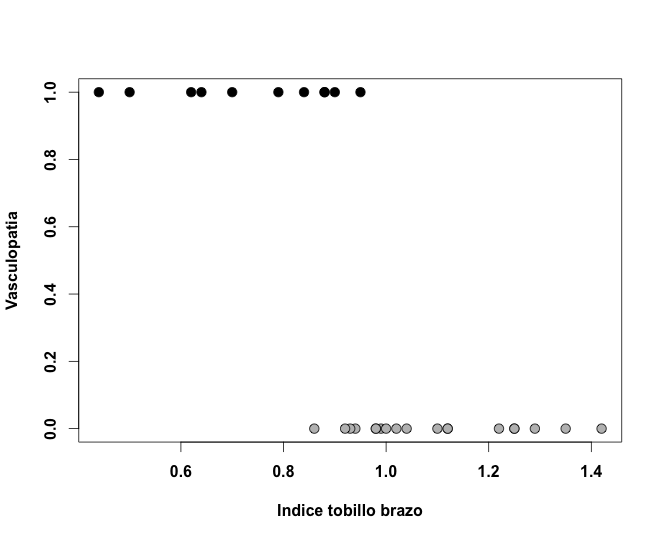
\includegraphics[width=11cm]{../fig/Cap13-DiagramaDispersionITB.png}
        \caption{Datos muestrales, de la Tabla \ref{cap13:TablaDatosVasculopatia}. }
		\label{cap13:fig:DiagramaDispersionITB}
		\end{center}
	\end{figure}

	
	Esta figura debe servir de motivación para empezar a preguntarnos qué tipo de modelo esperamos obtener en un problema como este.
	
	Antes de seguir adelante, queremos hacer una observación sobre este ejemplo: para fijar ideas, hemos empezado con una situación en la que valores bajos de la variable explicativa $X$ corresponden al valor $1$ del factor $Y$, mientras que los valores altos de la variable explicativa $X$ corresponden al valor $0$ del factor $Y$. En otros ejemplos podría ser al revés, pero eso no afecta a la esencia de la situación.
	\qed	
\end{ejemplo}


Para ayudarnos en esa reflexión, de nuevo puedes pensar en lo que hicimos en el Capítulo \ref{cap:RegresionLinealSimple} al tratar sobre los modelo de regresión lineal. En particular, queremos traer a tu memoria la terminología de {\em ruido y modelo} que hemos venido usando desde ese capítulo. Conviene que vuelvas a examinar la Figura \ref{cap10:fig:ErrorCuadraticoIgual0} (pág. \pageref{cap10:fig:ErrorCuadraticoIgual0}), en la que pensábamos en una situación en la que {\em todo es modelo y no hay presencia del ruido}.

¿Cuál es el equivalente aquí? Si lo pensamos un poco, la situación más sencilla posible ocurriría si existiera un {\sf valor umbral}\index{umbral, valor}\index{valor umbral} o {\sf valor de corte}\index{valor de corte} $x_u$ de la variable $X$, perfectamente definido, de
manera que pudiéramos decir:
\[
\begin{cases}
\mbox{ Si $X\leq x_u$ entonces $Y=1$.}\\[3mm]
\mbox{ Si $X>x_u$ entonces $Y=0$.}
\end{cases}
\]


\begin{ejemplo}
	\label{cap13:ejem:RegresionLogistica02}
	En el ejemplo de la relación \texttt{vasculopatía} \verb#~# \texttt{itb}, esa situación se daría si pudiéramos decir algo como: {\em ``todos los pacientes con itb mayor que $0.96$ (pongamos por caso)  presentan vasculopatía, y ningún paciente con itb menor que $0.96$ presenta vasculopatía}.  En ese caso el valor del itb permitiría una separación nítida entre los dos valores posibles (uno o cero) de la variable vasculopatía.
\qed
\end{ejemplo}

\noindent Este tipo de situaciones idealizadas se pueden representar mediante una {\sf función escalón inversa}\index{función escalón (directa o inversa)}\index{escalón, función}, como la de la parte (b) de la Figura \ref{cap13:FuncionEscalon}.  La parte (a) de la figura muestra una {\sf función escalón directa}, que corresponde a aquellos casos en los que los valores bajos de $X$ están asociados con el valor $X=0$ del factor.
\begin{figure}[htb]
\begin{center}
\begin{enColor}
\begin{tabular}{cc}
	    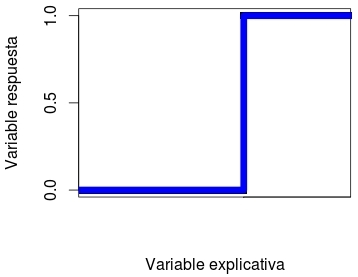
\includegraphics[width=6cm]{../fig/Cap13-QueEsperarEscalon1.png}&
	    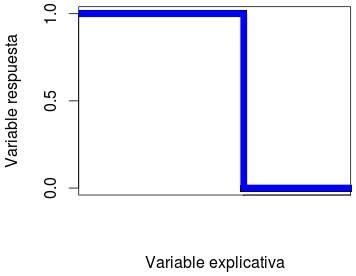
\includegraphics[width=6cm]{../fig/Cap13-QueEsperarEscalon2.png}\\[3mm]
	    (a) &   (b)\\[2mm]
\end{tabular}	
\end{enColor}
\begin{bn}
\begin{tabular}{cc}
	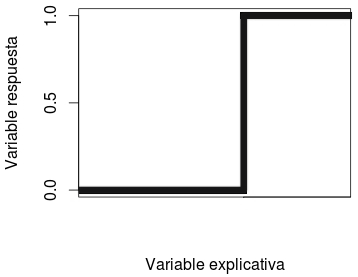
\includegraphics[width=6cm]{../fig/Cap13-QueEsperarEscalon1-bn.png}&
	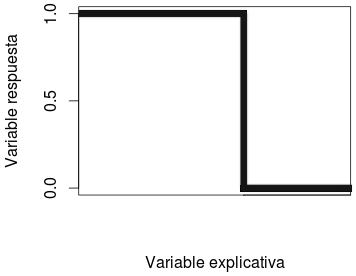
\includegraphics[width=6cm]{../fig/Cap13-QueEsperarEscalon2-bn.png}\\[3mm]
	(a) &   (b)\\[2mm]
\end{tabular}		
\end{bn}
     \caption{Gráficas de las funciones escalón: (a) directa y (b) inversa.}
     \label{cap13:FuncionEscalon}
\end{center}
\end{figure}

\noindent Estas funciones escalón aparecen en muchas situaciones, de las que los ejemplos más sencillos son los umbrales artificiales que los humanos fijamos en diversas situaciones: los niños menores de diez años no pagan entrada, los mayores sí. Aunque también hay situaciones naturales que se corresponden con escalones bastante parecidos a ese modelo ideal. Por ejemplo, las transiciones de fase. Si la variable explicativa $X$ es la temperatura, y consideramos un factor $Y$ con dos niveles, líquido (valor $0$) y gaseoso (valor $1$), entonces el comportamiento del agua se puede describir mediante una función escalón directa, como la de la Figura \ref{cap13:FuncionEscalon}(a), en la que el valor umbral es $x_u=100^\circ$C.

Esa es, por tanto, la situación que consideramos como representativa de {\em todo modelo, ningún ruido}. Pensemos ahora en lo que significan estas ideas, en el contexto del ejemplo que estamos utilizando.
\begin{ejemplo}
\label{cap13:ejem:RegresionLogistica03}
Si la relación entre el itb y el desarrollo o no de una vasculopatía se ajustara a un modelo ideal, con un valor umbral perfectamente definido, al examinar los valores de una muestra cabría esperar algo parecido a lo que aparece en la Figura \ref{cap13:fig:QueEsperarLogistica}, parte izquierda, (pág. \pageref{cap13:fig:QueEsperarLogistica}), con datos ficticios inventados para la ocasi\'on. En esa figura la relación sería {\em inversa}, es decir,
{\em todos} los individuos con un itb bajo desarrollan una vasculopatía mientras que, a partir del valor umbral, {\em ninguno} de los individuos ha desarrollado la vasculopatía. El caso simétrico, con una relación {\em directa}, se muestra en parte derecha de la figura para que puedas compararlo con la otra función escalón (pero recuerda que nuestros datos muestrales se parecen más a la figura de la izquierda).
\begin{figure}[h!]
\begin{center}
%    (a)\\[2mm]
    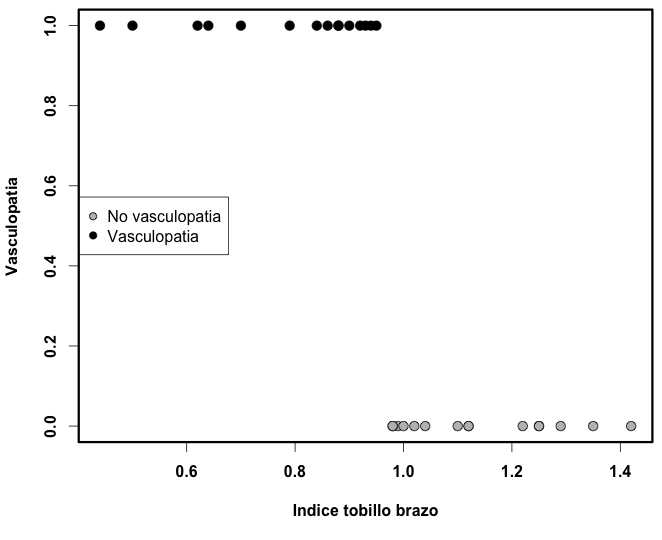
\includegraphics[width=6.5cm]{../fig/Cap13-QueEsperarLogistica2.png}%\\[2mm]
%    (b)\\[2mm]
    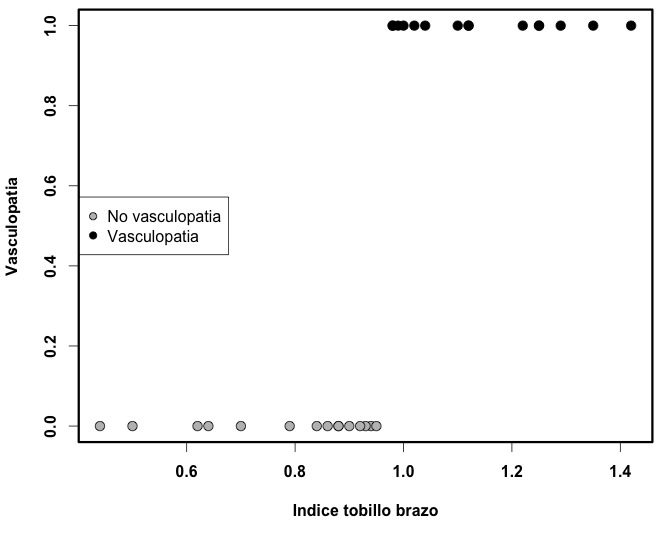
\includegraphics[width=6.5cm]{../fig/Cap13-QueEsperarLogistica1.png}%\\
     \caption{Situación idealizada del Ejemplo \ref{cap13:ejem:RegresionLogistica03}.
     	%En el eje horizontal se representa el itb de cada individuo. En el eje vertical, desarrollo (Vasculopatía = 1) o no (Vasculopatía = 0) de una vasculopatía. En figura de la izquierda la relación es inversa, mientras que en la figura de la  parte derecha es directa.
     	}
       \label{cap13:fig:QueEsperarLogistica}
   \end{center}
\end{figure}

Esto sería  lo que sucedería en un modelo sin ruido. ¿Qué ocurre en un caso más realista, como el de nuestra muestra, en el que interviene el {\em ruido} debido a los componentes aleatorios? Entonces lo que cabe esperar es un diagrama como el que hemos visto en la Figura \ref{cap13:fig:DiagramaDispersionITB} (pág. \pageref{cap13:fig:DiagramaDispersionITB}), que para mayor comodidad del lector hemos reproducido aquí como Figura \ref{cap13:fig:DiagramaDispersionITBrepe}. Vamos a analizar esa figura comparándola con las anteriores situaciones idealizadas. Se aprecia que:

	\begin{figure}[htb]
		\begin{center}
        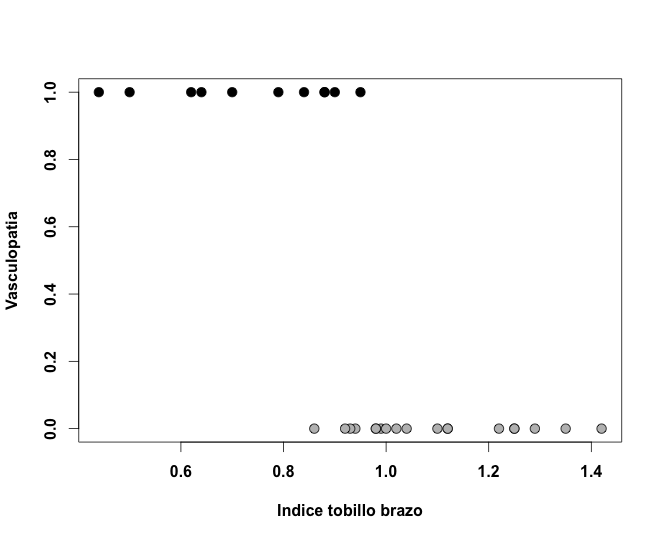
\includegraphics[width=11cm]{../fig/Cap13-DiagramaDispersionITB.png}
        \caption{Datos muestrales, de la Tabla \ref{cap13:TablaDatosVasculopatia}. }
		\label{cap13:fig:DiagramaDispersionITBrepe}
		\end{center}
	\end{figure}


\begin{itemize}
  \item Todos los pacientes con itb menor que $0.8$ han desarrollado vasculopatía.

  \item A partir de cierto valor dado del itb (por ejemplo itb=$1.1$), ninguno de los paciente ha desarrollado vasculopatía.

  \item {\bf Y lo más importante:} también está claro que hay una {\em zona de transición}, de valores de itb cercanos a $1$, en los que se entremezclan casos de vasculopatía con otros en los que no aparece la  enfermedad. Es decir, que los valores $Y=1$ e $Y=0$ se alternan mientras dura esa transición y no hay un valor de $X$ que permita separarlos limpiamente .

  %\item La {\em gran mayoría} de los casos con itb {\em suficientemente bajo} hayan desarrollado vasculopatía. Pero algunos, en un porcentaje bajo, no la habrán desarrollado (por razones genéticas, ambientales o de cualquier otro tipo, que no estamos considerando en el estudio).


 % \item Análogamente, la {\em gran mayoría} de los casos con itb {\em suficientemente alto} no habrán desarrollado vasculopatía.

  %\item En lugar de un valor umbral perfectamente definido, ahora esperamos encontrar un solapamiento de los casos, una {\sf zona de transición} en los valores de itb, en la que el porcentaje de casos de vasculopatía va disminuyendo, a medida que el valor del itb aumenta. Pero, insistimos, la transición ocurre durante un intervalo de valores. Los casos no están nítidamente separados, de manera que a medida que el itb aumenta, los valores $1$ y $0$ alternan durante un intervalo más o menos amplio.
\end{itemize}

%Con esto, estamos listos para visualizar en un gráfico los datos reales de la muestra, los que ya vimos en la Tabla \ref{cap13:TablaDatosVasculopatia}
%(pág. \pageref{cap13:TablaDatosVasculopatia}). Ese gráfico aparece en la
%Figura \ref{cap13:RegresionLogisticaEj} (pág. \pageref{cap13:RegresionLogisticaEj}).
%
%\begin{figure}[h!]
%\begin{center}
%   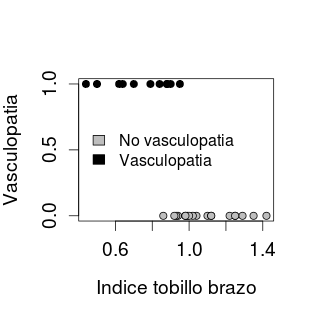
\includegraphics[height=6cm]{../fig/Cap13-Vasculopatia.png}
%    \caption{Datos muestrales, de la Tabla \ref{cap13:TablaDatosVasculopatia}. En el eje vertical, la presencia (1) o no (0) de una vasculopatía. Los datos sugieren que hay más casos de vasculopatía asociados a itb bajos. }
%    \label{cap13:RegresionLogisticaEj}
%\end{center}
%\end{figure}

La Figura \ref{cap13:fig:DiagramaDispersionITBrepe} confirma las sospechas de los investigadores, en un sentido parecido a lo que ocurría con la Figura \ref{cap10:fig:Herrerillo} (pág. \pageref{cap10:fig:Herrerillo}) en el Capítulo \ref{cap:RegresionLinealSimple}.

Para tener una visión más completa de la situación, ahora conviene que nos preguntemos: ¿qué esperaríamos ver si no hubiera ninguna relación entre el itb y el desarrollo de una vasculopatía? Es decir, ¿cuál es la situación que podríamos interpretar como {\em todo ruido y nada de modelo}? En ese caso, los valores $1$ y $0$ aparecerían aleatoriamente para cualquier valor de itb. Usando datos simulados, hemos representado esa situación en la Figura \ref{cap13:fig:RegresionLogisticaNoRelacion}.
\begin{figure}[h!]
\begin{center}
    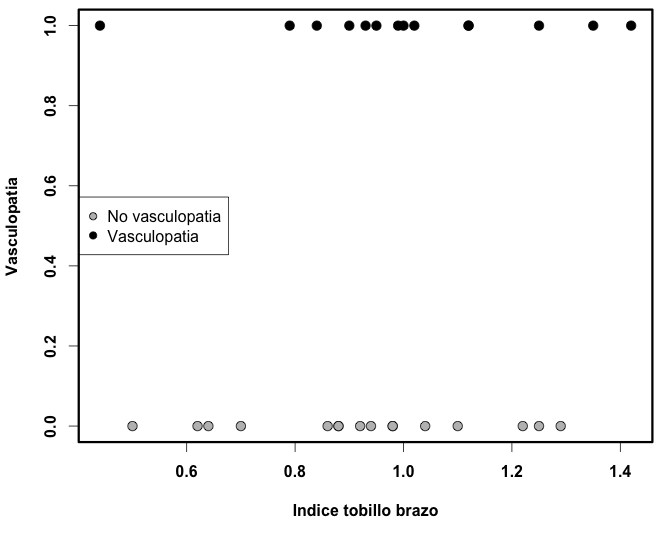
\includegraphics[width=13cm]{../fig/Cap13-VasculopatiaNoRel.png}
\end{center}
\caption{El caso ``todo ruido, nada de modelo'' en el Ejemplo \ref{cap13:ejem:RegresionLogistica03}.}
\label{cap13:fig:RegresionLogisticaNoRelacion}
\end{figure}
La distribución de los datos de la figura sugiere que la enfermedad parece no guardar relaci\'on con el valor del itb, pues los casos aparecen, aproximadamente, uniformemente repartidos en el recorrido de los valores del itb. Siguiendo con las analogías que estamos estableciendo con el modelo de regresión lineal, esta situación nos recuerda a la del diagrama de dispersión de la Figura \ref{cap10:fig:EjemploRectaMalaAproximacion02} (pág. \pageref{cap10:fig:EjemploRectaMalaAproximacion02}), en la que quedaba patente la falta de una relación clara entre las variables. La diferencia entre ambas figuras es, insistimos, que las coordenadas verticales, ahora, en la Figura \ref{cap13:fig:RegresionLogisticaNoRelacion}, sólo pueden valer $0$ o $1$.
\qed
\end{ejemplo}

Teniendo en cuenta las ideas que hemos ido exponiendo en estos ejemplos. ¿Qué clase de respuesta  esperamos de un {\em modelo} en este tipo de situaciones, qué tipo de {\em predicción}? Concretamente, imagínate que acudimos a nuestro modelo con un valor de la variable $X$. Una primera idea ingenua es que al introducir ese valor en el modelo podríamos obtener $1$ o $0$ como respuesta.  Eso sería suficiente en los casos en los que existe un umbral claramente definido en los valores de $X$ que separa unos casos de otros. Pero cuando existe la {\em zona de transición} que hemos visto en los ejemplos, esta respuesta no puede ser satisfactoria. ¿Qué deberíamos hacer entonces? La solución consiste en no centrarse \emph{en los valores} de $Y$ ( los unos y ceros) y pensar, en cambio, en la {\em probabilidad} de que $Y$ tome uno de esos valores.  Es un cambio trascendental, que afecta a la estructura del modelo que vamos a construir. La pregunta a la que vamos a responder \textbf{no} es esta:
\begin{center}
	\emph{Dado un valor $x_0$ de $X$,  ¿cuál es el valor de $Y$, uno o cero?}
\end{center}
sino esta otra:
\begin{center}
	\emph{Dado un valor $x_0$ de $X$,  ¿cuál es la probabilidad de que $Y$ tome el valor  uno?}
\end{center}
Es decir, que el objeto central de nuestro modelo es una probabilidad condicionada:
\[P(Y | X= x_0).\]
Ten en cuenta que, desde luego, se tiene
\[P(Y=0|X=x_0)= 1 - P(Y=1|X=x_0),\]
así que basta con calcular la probabilidad condicionada para el valor $Y=1$.

Al principio puede costarte un poco entender el cambio de punto de vista que se produce al hacer esto, pero pronto, con la ayuda de los ejemplos, empezarás a ver cómo funciona. La intuición que hay detrás de ese cambio de pregunta corresponde a lo que hemos discutido sobre la Figura \ref{cap13:fig:DiagramaDispersionITBrepe} (pág. \pageref{cap13:fig:DiagramaDispersionITBrepe}). Cuando el valor $x_0$ es grande (en la parte derecha de la gráfica), la probabilidad de que $Y$ tome el valor $1$ es prácticamente igual a $0$. Dicho de otro modo,  todos los valores de $Y$ para $x_0$ suficientemente a  la derecha son $0$. Por contra, en la parte izquierda de la gráfica, la probabilidad de $Y=1$ es casi igual a $1$ (todos los valores de $Y$ para $x_0$ suficientemente a  la izquierda son $1$).   ¿Y en la zona de transición? ¿Qué ocurre ahí con la probabilidad $P(Y = 1| X= x_0)$? Pues ahí esperamos que ocurra eso, una transición, de manera que, a medida que $x_0$ se hace más grande, el valor de la probabilidad descienda desde $1$ hasta $0$.  Pero siempre teniendo presente que ahora hablamos de probabilidades.

Así, por ejemplo, puede ocurrir que para un $x_0$ en la zona de transición nuestro modelo prediga
\[P(Y = 1 | X= x_0) = 0.75.\]
Eso significa que de cada cuatro observaciones con un valor $X=x_0$, esperamos que en tres de ellas se cumpla $Y=1$. Pero también esperamos que, \emph{con ese mismo valor $x_0$,} una cuarta parte de las observaciones correspondan a valores $Y=0$. Nuestro modelo, insistimos, no va a predecir valores de $Y$ sino probabilidades de esos valores.

\subsection{Agrupando valores para estimar las probabilidades.}
\label{cap13:subsec:AgrupandoValoresEstimarProbabilidades}

Ahora ya tenemos más claramente definido nuestro objetivo: calcular, para cada valor dado $x_0$ de la variable explicativa $X$, cuál es la probabilidad de que la variable respuesta $Y$ tome el valor $1$. Dicho de otra forma, si sabemos que el valor de la variable $X$ es $x_0$, \textquestiondown qué probabilidad hay de que, en esa observación sea $Y=1$? En términos de la probabilidad condicionada, estamos intentando predecir la probabilidad:
	\begin{equation}
    \label{cap13:ecu:ProbLogistica}
    P(Y=1|X=x_0).
	\end{equation}

¿Cómo podríamos estimar, a partir de la muestra, esa probabilidad condicionada? Recuerda que,
como advertimos en la página \pageref{cap13:ejem:RegresionLogistica00} (antes de empezar con el
Ejemplo \ref{cap13:ejem:RegresionLogistica00}), la variable $X$, que es cuantitativa, puede ser
continua o discreta. Si es continua, como hemos venido suponiendo en los ejemplos previos, las matemáticas del cálculo de probabilidades se complica: tendremos que construir una función que nos diga cuánto vale la probabilidad para cada uno de los infinitos valores posibles $x_0$). Dejando esto para más adelante, inicialmente vamos a optar por un
camino mucho más sencillo y que conocemos desde el principio del curso. La idea es la misma que
utilizamos cuando, en la Sección \ref{cap01:subsec:NotacionVariablesTablasFrecuenciaDatosAgrupados}
(pág. \pageref{cap01:subsec:NotacionVariablesTablasFrecuenciaDatosAgrupados}) del Capítulo
\ref{cap:IntroduccionEstadisticaDescriptiva} hablamos de {\em datos (continuos) agrupados en
clases}. Es la idea que usamos para representar los datos en un histograma, y que en el fondo se
reduce a:

\begin{itemize}

  \item Dividir los posibles valores de la variable en intervalos, llamados {\em clases}, y

  \item Representar todos los valores de la clase (intervalo) $(a,b]$ mediante la llamada {\em marca de clase}:
      \[\dfrac{a+b}{2}.\]
\end{itemize}
Usando esta idea (que es una {\em discretización} de la variable continua), podemos utilizar el procedimiento que se describe a continuación. Enseguida  veremos un ejemplo; si te resulta más sencillo, puedes ir avanzando por los pasos del procedimiento a la vez que lees el Ejemplo \ref{cap13:ejem:EstimacionModeloLogisticoMedianteClases}:
\begin{enumerate}
  \item Dividimos el recorrido de valores de la variable $X$ en $k$ clases:
  \[(u_0,u_1],\quad (u_1,u_2],\quad (u_2,u_3],\cdots,\quad (u_{k-1},u_k],\]
  cuyas marcas de clase son
  \[w_i=\dfrac{u_{i-1}+u_{i}}{2}\mbox{ para }i=1,\ldots, k.\]
  \item Para cada clase $(u_{i-1},u_i]$, localizamos aquellos puntos $(x_j,y_j)$ de la muestra tales que $x_j$ pertenece a esa clase.
  \item Supongamos que hay  $n_i$ de esos puntos. Una parte de ellos tendrán valores de $Y$ iguales a $1$, y el resto tendrán valores iguales a $0$. Vamos a llamar $o_i$ al número de puntos (de esa clase) cuyo valor de $Y$ es $1$ (la notación pretender recordarte a la que hemos usado en el contraste $\chi^2$ de homogeneidad). Entonces el cociente:
      \begin{equation}
      \label{cap13:ecu:EstimacionProbabilidadFactorIgual1EnUnaClase}
        \hat p_i=\dfrac{o_i}{n_i}
      \end{equation}
      sirve como estimación de la probabilidad condicionada $P(Y=1|X=x_0)$ de la Ecuación \ref{cap13:ecu:ProbLogistica}, cuando $x_0$ pertenece a la clase número $i$.

  \item Al hacer esto para cada una de las clases, tendremos una colección de $k$ puntos, uno por cada clase,
      \[(w_1,\hat p_1),\, (w_2,\hat p_2),\,\ldots,\, (w_k,\hat p_k),\]
      formados por las marcas de clase, y las estimaciones de $P(Y=1|X=x_0)$ para $x_0$ en esa clase.
\end{enumerate}
Veamos el ejemplo prometido:
\begin{ejemplo}
\label{cap13:ejem:EstimacionModeloLogisticoMedianteClases}
Después volveremos a los datos de la relación entre itb y la vasculopatía. Pero, dado que ese ejemplo tiene una cantidad relativamente pequeña de puntos, para ilustrar este paso vamos a utilizar un ejemplo con una gran cantidad de puntos. Concretamente, el fichero adjunto:
\begin{center}
\fichero{../datos/Cap13-ConstruccionModeloLogistico.csv}{Cap13-ConstruccionModeloLogistico.csv}
\end{center}
contiene una tabla de $1000$ observaciones (en las dos primeras columnas), cada una de la forma $(x_i,y_i)$, donde $x_i$ es el valor de la variable explicativa $X$ (cuantitativa continua) e $y_1$ es el valor de la variable respuesta $Y$, un factor con dos valores posibles, $1$ y $0$. La Figura \ref{cap13:fig:EjemploConstruccionModeloLogistico01} muestra esos valores. Como puede verse, parecen apuntar a una relación directa entre ambas variables, con una zona de solapamiento en la parte central del gráfico. Veamos, paso a paso, como se aplica a estos datos el procedimiento que hemos descrito.

\begin{figure}[h!]
\begin{center}
\begin{enColor}
   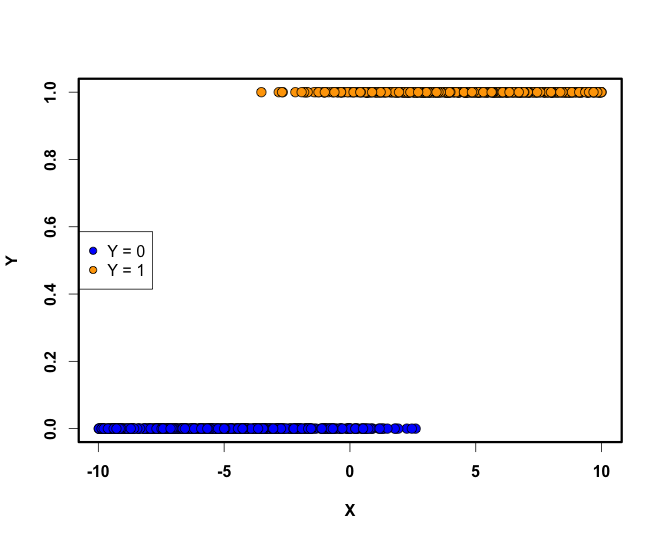
\includegraphics[width=13cm]{../fig/Cap13-EjemploConstruccionModeloLogistico01.png}
\end{enColor}
\begin{bn}
    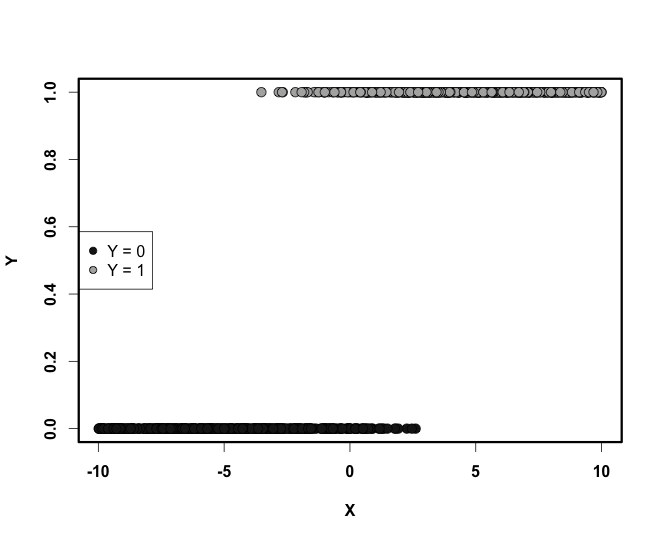
\includegraphics[width=13cm]{../fig/Cap13-EjemploConstruccionModeloLogistico01-bn.png}
\end{bn}
\end{center}
    \caption{ Datos muestrales del Ejemplo \ref{cap13:ejem:EstimacionModeloLogisticoMedianteClases}. }
    \label{cap13:fig:EjemploConstruccionModeloLogistico01}
\end{figure}
\begin{enumerate}
  \item Como puede verse en la figura, el intervalo $[-10,10]$ de valores de la variable $X$ contiene completamente la que hemos llamado {\em zona de transición}. En la zona situada más a la izquierda del intervalo $[-10,10]$ todos los valores de $Y$ son iguales a $0$, y en la zona más a la derecha, todos son iguales a $1$. Así que podemos tomar ese intervalo como base para el modelo. Empezamos dividiendo el intervalo $[-10,10]$ en $40$ clases, de anchura $1/2$:
      \[[-10,-9.5], \,(-9.5,-9],\, (-9,-8.5],\, \ldots, \,(9,9.5], \,(9.5,10].\]
      Es decir, que
      \[u_0=-10,\, u_1=-9.5,\,\ldots,\,u_i=-10+i\cdot\dfrac{1}{2},\,\ldots,\,u_{40}=10.\]
      Las marcas de clase serán los puntos:
      \[w_1=-9.75,\,w_2=-9.25,\,w_3=-8.75,\,\ldots,\,w_{40}=9.75.\]
      ¿Cuántas clases debemos utilizar? Esa pregunta es parecida a la que nos hicimos al agrupar los datos en el Capítulo \ref{cap:IntroduccionEstadisticaDescriptiva}, o al construir el histograma en el Capítulo \ref{cap:ValoresCentralesDispersion}. Y, como en esos dos casos, por ahora no vamos a dar una respuesta demasiado concreta: el número de clases que convenga. Aquí tenemos una muestra con un número muy elevado de puntos, que además queremos usar a efectos de ilustrar la idea. Por eso hemos podido tomar un número alto de clases, a sabiendas de que en este caso el detalle de lo que sucede será fácil de apreciar. En la Sección \ref{cap13:sec:BondadDelAjuste}, cuando tengamos más claro cómo es el modelo, volveremos sobre estas mismas ideas con mucho más detalle.
  \item Ahora, para cada una de esas $40$ clases, hacemos un recuento del numero de puntos muestrales cuya coordenada $X$ pertenece a esa clase. Por ejemplo, si miramos la clase número $5$ (ver el Tutorial13), que es el intervalo $(-8,-7.5]$, descubriremos que hay $27$ puntos de la muestra con
      \[-8<X\leq -7.5.\]
      Esa clase está ubicada muy a la izquierda en el intervalo $[-10,10]$. De hecho, los valores $Y$ de esos $27$ puntos muestrales son {\em todos} iguales a $0$. De la misma forma, si tomamos una clase ubicada muy a la derecha, como la clase $(7,7.5]$ (que hace el número $35$ de las $40$ que hay), entonces descubriremos que hay $23$ puntos muestrales con coordenada $X$ en esa clase, pero que todos ellos tienen coordenada $Y$ igual a $1$.\\
      Las clases {\em ``interesantes''} son las de la zona de transición. Fijémonos, por ejemplo, en la clase número $18$, que es el intervalo $(-1.5,-1]$. Hay $17$ puntos muestrales con coordenada $X$ en esa clase. Concretamente, son los que aparecen en la Tabla \ref{cap13:tabla:Clase18EjemploModeloMedianteClases} (divididos en dos, porque la tabla es demasiado ancha para caber en una fila). Los valores de $Y$ ahora son ceros y unos  mezclados.
        \begin{table}[ht]
        \centering
        {\small
        \begin{tabular}{rrrrrrrrrr}
          \hline
        X & -1.02 & -1.13 & -1.35 & -1.15 & -1.23 & -1.43 & -1.00 & -1.34 & -1.01 \\
        \hline
          Y & 0 & 0 & 1 & 0 & 1 & 1 & 0 & 0 & 0 \\
           \hline
           \hline
         X  & -1.04 & -1.06 & -1.42 & -1.06 & -1.07 & -1.05 & -1.25 & -1.12 \\
         \hline
         Y & 1 & 0 & 0 & 0 & 0 & 1 & 1 & 0 \\
         \hline
        \end{tabular}
        }
        \caption{Puntos de la clase $(-1.5,1]$ del Ejemplo \ref{cap13:ejem:EstimacionModeloLogisticoMedianteClases}.}
        \label{cap13:tabla:Clase18EjemploModeloMedianteClases}
        \end{table}
  \item Vamos a usar como ejemplo inicial las tres clases en las que nos hemos fijado en el paso anterior. Para la clase $(-8,-7.5]$ (clase número $5$) hemos visto que:
      $n_{5}=27$, $o_i=0$, porque no hay ningún punto con $Y=1$ en esos $27$. Así que nuestra estimación $\hat p_{5}$, de la probabilidad sólo puede ser:
      \[P(Y=1|-8<X\leq 75)\approx \hat p_5=\dfrac{0}{27}=0.\]
      Para la clase $(7,7.5]$ (clase número $35$) hemos visto que:
      $n_{35}=23$, $o_i=23$, así que la estimación de la probabilidad es, obviamente:
      \[P(Y=1|X\mbox{ en esa clase})\approx \hat p_{35}=\dfrac{23}{23}=1.\]
      Para la clase más ``interesante'', la $(-1.5,-1]$, que hace el número $18$, hemos obtenido (ver la Tabla \ref{cap13:tabla:Clase18EjemploModeloMedianteClases}):
      $n_{18}=17$, $o_i=6$, así que la estimación de la probabilidad es:
      \[P(Y=1|X\mbox{ en esa clase})\approx \hat p_{18}=\dfrac{6}{17}\approx 0.3529.\]

  \item Una vez calculados todos los valores $\hat p_1,\ldots, \hat p_{40}$, representamos los $40$ puntos
      \[(w_1,\hat p_1), \ldots, (w_{40},\hat p_{40}),\]
      (recuerda que los $w_i$ son las marcas de clase), junto con los valores muestrales que ya vimos en la Figura \ref{cap13:fig:EjemploConstruccionModeloLogistico01} (pág. \pageref{cap13:fig:EjemploConstruccionModeloLogistico01}). El resultado está en la Figura \ref{cap13:fig:EjemploConstruccionModeloLogistico02}.
\begin{figure}[h!]
\begin{center}
\begin{enColor}
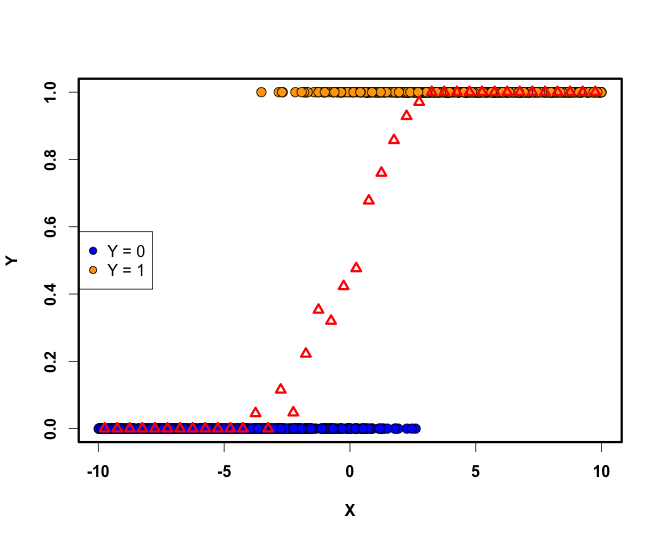
\includegraphics[width=13cm]{../fig/Cap13-EjemploConstruccionModeloLogistico02.png}
\end{enColor}
\begin{bn}
    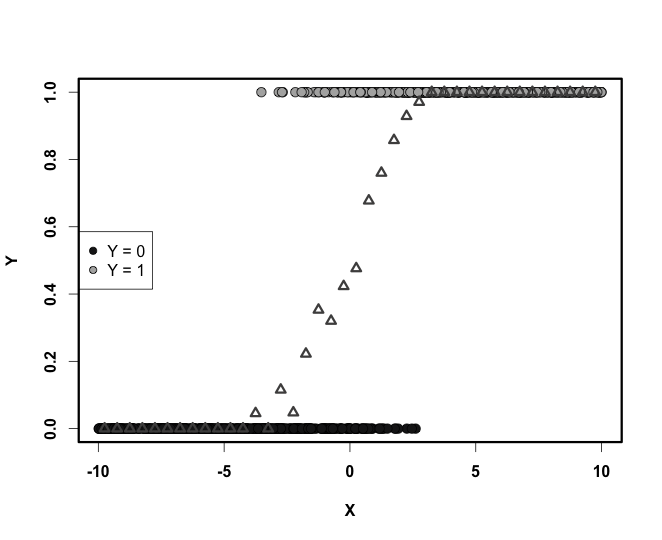
\includegraphics[width=13cm]{../fig/Cap13-EjemploConstruccionModeloLogistico02-bn.png}
\end{bn}
\caption{Predicción de probabilidades por clases para el Ejemplo \ref{cap13:ejem:EstimacionModeloLogisticoMedianteClases}. }
\label{cap13:fig:EjemploConstruccionModeloLogistico02}
\end{center}
\end{figure}

    Los triángulos rojos que aparecen en la figura son las estimaciones de la probabilidad
    condicionada para cada clase. Y como puedes ver, las estimaciones parecen colocarse a lo
    largo de una curva con forma de s, una {\em curva sigmoidea}.
\end{enumerate}
\qed
\end{ejemplo}
\noindent La curva sigmoidea que hemos intuido en este ejemplo apunta al {\em modelo de regresión
logística}. Es decir, nuestro objetivo, en un problema como el que hemos descrito en los ejemplos
de esta sección, será encontrar una de estas curvas sigmoideas que describa, para cada valor $x_0$
de la variable $X$, cuánto vale la probabilidad condicionada
\begin{equation}
\label{cap13:ecu:NotacionPiProbabilidadCondicionada}
\pi(x_0)=P(Y=1|X=x_0).
\end{equation}
Las cosas pueden ser, en todo caso, aún más complicadas de lo que sugieren los ejemplos que hemos visto hasta ahora. Para ilustrar lo que queremos decir, vamos a presentar de forma muy breve, un ejemplo adicional.
\begin{ejemplo}
\label{cap13:ejem:EstimacionModeloLogisticoVariasInflexiones}
El fichero adjunto
\begin{center}
  \fichero{../datos/Cap13-ConstruccionModeloLogistico-Inflexiones.csv}{Cap13-ConstruccionModeloLogistico-Inflexiones.csv}
\end{center}
contiene una tabla de datos similar a la que hemos visto en el Ejemplo \ref{cap13:ejem:EstimacionModeloLogisticoMedianteClases} (pág. \pageref{cap13:ejem:EstimacionModeloLogisticoMedianteClases}). Pero si repetimos el mismo esquema que hemos aplicado allí (la división de los datos en clases aparece en el fichero de datos), para calcular los correspondientes puntos $(w_i, \hat p_i)$, obtenemos la Figura
\ref{cap13:fig:ModeloLogisticoVariasInflexiones}. Como se aprecia en esa figura, los puntos $(w_i, \hat p_i)$ no se disponen a lo largo de una curva sigmoidea simple, como la que insinúa la Figura \ref{cap13:fig:EjemploConstruccionModeloLogistico02} (pág. \pageref{cap13:fig:EjemploConstruccionModeloLogistico02}).
\begin{figure}[h!]
\begin{center}
\begin{enColor}
    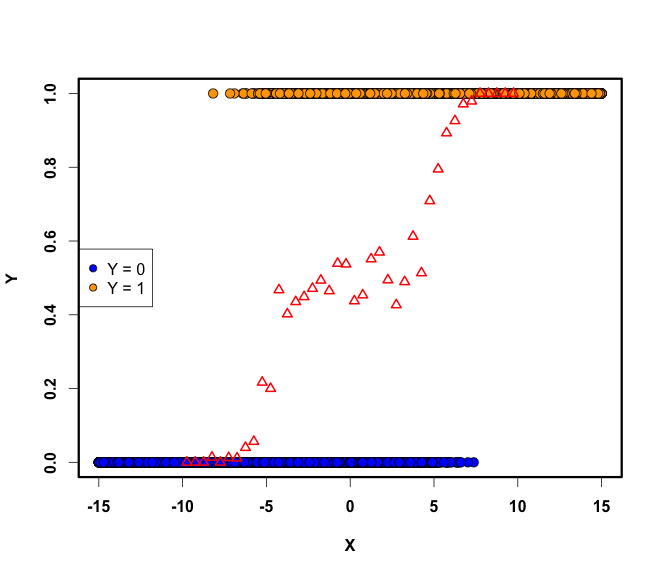
\includegraphics[width=11cm]{../fig/Cap13-EstimacionModeloLogisticoVariasInflexiones.png}
\end{enColor}
\begin{bn}
    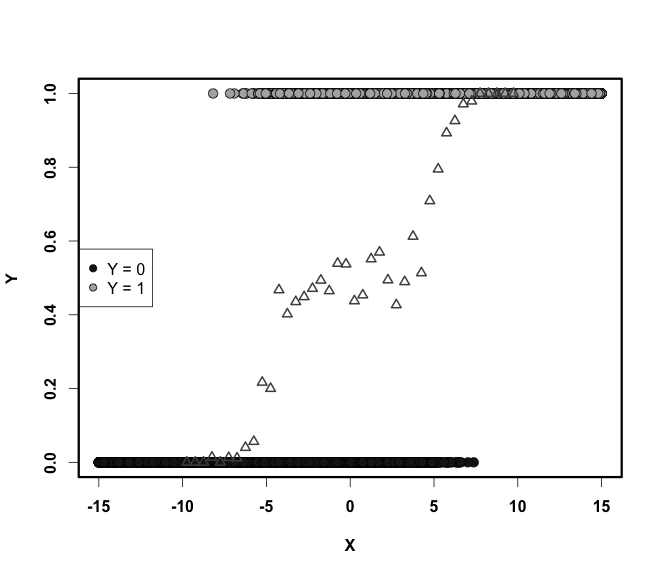
\includegraphics[width=11cm]{../fig/Cap13-EstimacionModeloLogisticoVariasInflexiones-bn.png}
\end{bn}
\caption{Los datos originales y los puntos $(w_i, \hat p_i)$ del Ejemplo \ref{cap13:ejem:EstimacionModeloLogisticoVariasInflexiones}. }
\label{cap13:fig:ModeloLogisticoVariasInflexiones}
\end{center}
\end{figure}

Por el contrario, la curva de la Figura \ref{cap13:fig:ModeloLogisticoVariasInflexiones} nos recuerda a una situación como la de la Figura \ref{cap05:fig:TipicaFuncionDistribucionVariableContinua} (pág. \pageref{cap05:fig:TipicaFuncionDistribucionVariableContinua}).
\qed
\end{ejemplo}

\noindent El mensaje que queremos transmitir, con este último ejemplo, es que en la regresión logística nos vamos a encontrar con un problema similar al que ilustraba la Figura \ref{cap10:fig:EjemploRectaMalaAproximacion01} (pág. \pageref{cap10:fig:EjemploRectaMalaAproximacion01}) en el caso de la regresión lineal. Allí aprendimos que, aunque siempre seamos capaces de construir la recta de regresión, esa recta no siempre será la mejor manera de describir la relación entre las dos variables. Incluso cuando es evidente que esa relación existe. Trasladando esa lección al contexto de este capítulo, incluso aunque seamos capaces de encontrar {\em la mejor curva sigmoidea posible}, bien podría suceder que los datos no se describan adecuadamente mediante una curva tan sencilla como es una curva sigmoidea. Los ejemplos como el de la Figura \ref{cap13:fig:ModeloLogisticoVariasInflexiones} indican claramente que, en algunos casos, se necesitan modelos más sofisticados (con curvas capaces de incorporar varios cambios de concavidad, etc.)\\

\subsubsection*{Recapitulando.}

\noindent El trabajo que hemos hecho en esta sección nos plantea dos problemas inmediatos:
\begin{enumerate}

   \item ¿Cómo construimos la {\em ``mejor curva sigmoidea''}, la que mejor se ajusta a nuestra muestra, en el sentido de que es la que mejor describe las probabilidades? Este paso es análogo a la
       construcción de la recta de regresión lineal a partir de una nube de puntos, que hicimos
       en la Sección \ref{cap10:subsec:ComoElegirLaMejorRecta}. Esta tarea, a su vez, tiene un requisito preliminar. Para poder construir la mejor curva, primero tenemos que dejar claro cuál es el criterio que usaremos para comparar dos curvas y decir que una es mejor que la otra. En el caso de la regresión lineal hemos usado sobre todo el criterio de mínimos cuadrados. Pero también vimos que esa no era la única posibilidad (por ejemplo, podíamos usar regresión ortogonal).

   \item Una vez elegido ese criterio y construida la mejor curva sigmoidea posible, todavía tenemos que aprender a  medir la {\em bondad del ajuste} de esa curva a los datos. En el Capítulo       \ref{cap:RegresionLinealSimple}, la calidad del ajuste se examinaba mediante la identidad Anova. Aquí hemos usado expresamente la expresión {\em bondad del ajuste} porque,  recuerda, $Y$ es un factor, y no hay varianza para los factores (ni, por tanto, Anova). Por esa razón, la calidad del ajuste se medirá, en este caso, por  una técnica estrechamente emparentada con el contraste $\chi^2$ de homogeneidad (o de bondad del ajuste), que hemos discutido en la Sección \ref{cap12:sec:ChiCuadradoHomgeneidad}.

 \end{enumerate}
En las siguientes secciones responderemos a estas cuestiones.

\section{La curva de regresión logística.}
\label{cap13:sec:CurvaLogistica}

Con la notación de la Ecuación \ref{cap13:ecu:NotacionPiProbabilidadCondicionada} (pág. \pageref{cap13:ecu:NotacionPiProbabilidadCondicionada}), lo que queremos es estimar el valor de
\[
\pi(x)=P(Y=1|X=x),
\]
en lugar de predecir el valor de $Y$ (que, en cualquier caso, es $1$ o $0$).
Nuestro plan para estimar esa probabilidad consiste en utilizar un modelo basado en una curva de regresión sigmoidea como la que aparece en la Figura \ref{cap13:fig:EjemploConstruccionModeloLogistico02}
(pág \pageref{cap13:fig:EjemploConstruccionModeloLogistico02}). Partiendo de un conjunto de datos observados

Dada una colección de puntos (como los puntos $(w_i,\hat p_i)$ del Ejemplo \ref{cap13:ejem:EstimacionModeloLogisticoMedianteClases}, pág. \pageref{cap13:ejem:EstimacionModeloLogisticoMedianteClases}) ¿Cómo podemos localizar la {\em ``mejor curva sigmoidea posible''}? Esta pregunta es parecida a la que nos hicimos en el caso de la regresión lineal, en el Capítulo \ref{cap:RegresionLinealSimple}, cuando buscábamos la {\em ``mejor recta posible''}. Pero hay una diferencia muy importante entre ambas situaciones: mientras que las rectas son todas esencialmente iguales entre sí, las  curvas sigmoideas pueden ser muy distintas unas de otras. Es decir, que mientras una ecuación de la forma
\[y = b_0 + b_1\cdot x\]
describe a {\em todas} las rectas posibles (salvo las verticales), con las curvas sigmoideas las cosas no tan sencillas. Hay muchas familias distintas de curvas sigmoideas, y la elección de una de esas familias condiciona de manera fundamental el trabajo de construcción del modelo.

Para que quede más claro, vamos a recordar algunas situaciones en las que nos hemos encontrado con curvas sigmoideas. Dentro del catálogo de curvas que ya hemos manejado en este curso, muchas funciones de distribuci\'on de probabilidad de variables aleatorias continuas tienen
forma sigmoidea. Puedes ver una ilustración de esto en la Figura
\ref{cap05:fig:FuncionDistribucionCauchy} (pág.  \pageref{cap05:fig:FuncionDistribucionCauchy}).
Recuerda, sin embargo, que esto no es cierto para todas las funciones de distribuci\'on, como pon\'ian de manifiesto las Figuras \ref{cap05:fig:TipicaFuncionDistribucionVariableContinua}
(pág.  \pageref{cap05:fig:TipicaFuncionDistribucionVariableContinua}) y
\ref{cap05:fig:EjemploFuncionDistribucionDensidadSoporteIntervalos02}
(pág.  \pageref{cap05:fig:EjemploFuncionDistribucionDensidadSoporteIntervalos02}).
Pero, para evitar eso, podemos asegurarnos de que usamos una colección de funciones de distribución adecuadas, para garantizar que son funciones sigmoideas sencillas, como la de la Figura
\ref{cap05:fig:FuncionDistribucionCauchy}). Concretamente, podríamos hacer esto:
\begin{itemize}
  \item Dada una distribución normal $N(\mu,\sigma)$, sea $\Phi_{\mu,\sigma}$ su función de distribución (la notación $\Phi_{\mu,\sigma}$\index{$\Phi_{\mu,\sigma}$} se introdujo en la página \pageref{ch06:ecu:NotacionPhiFuncionDistribucionZ}). Todas las curvas $\Phi_{\mu,\sigma}$ son curvas sigmoideas sencillas, cuya forma y posición depende de los valores de $\mu$ y $\sigma$ (de la misma manera que la forma y posición de la recta dependen de los valores de $b_0$ y $b_1$).
  \item Dada una colección de puntos $(w_i,\hat p_i)$, podemos buscar los valores de $\mu$ y $\sigma$ que producen la curva sigmoidea $\Phi_{\mu,\sigma}$ que mejor se ajusta a esos puntos. Este paso es parecido a lo que hicimos en el caso de la regresión lineal simple, cuando buscábamos los valores de $b_0$ y $b_1$ que producían la mejor recta.
\end{itemize}
Podríamos hacer esto y, de hecho, en ocasiones se hace (en los llamados modelos {\sf probit}\index{probit}). Pero hay un problema: las funciones $\Phi_{(\mu,\sigma)}$ son muy complicadas, y trabajar con ellas no es especialmente cómodo. Esta dificultad proviene del hecho de que la distribución normal no tiene una primitiva elemental, como ya vimos en la Sección \ref{cap05:sec:DistribucionNormalTCL} (pág. \pageref{cap05:sec:DistribucionNormalTCL}). Este hecho constituye una complicación innecesaria para la discusión que nos traemos entre manos. Volveremos un poco más adelante (y muy brevemente) sobre este enfoque cuando hablemos de funciones de enlace.

Afortunadamente, hay otras alternativas: los matemáticos disponen de un amplio catálogo de curvas sigmoideas que incluye una familia de curvas especialmente sencillas y, por lo tanto, adecuada a nuestros propósitos. De hecho, esta familia es la que da nombre a la técnica.


\begin{center}
    \fcolorbox{black}{Gris025}{
    \begin{minipage}{10cm}
        \begin{center}
        %%%%%%%%%%%%%%%%%%%%%%%%%%%%%%%%%%%%%%%
        {\bf  Curvas logísticas.}
        \end{center}
        \index{curva logística}\index{logística, curva}
        %%%%%%%%%%%%%%%%%%%%%%%%%%%%%%%%%%%%%%%
        La familia de curvas logísticas se define como sigue:
          \begin{equation}\label{cap13:EcCurvaLogistica1}
        	w=f(v)=\dfrac{e^{b_0+b_1 v}}{1+e^{b_0+b_1 v}}.
          \end{equation}
          donde $b_0, b_1$ son números cualesquiera.
        %%%%%%%%%%%%%%%%%%%%%%%%%%%%%%%%%%%%%%%
    \end{minipage}}
    \end{center}

Para empezar, observa que el denominador es una unidad mayor que el numerador, por lo que
$f(v)$ se mantiene siempre entre $0$ y $1$. Hay que advertir que, en bastantes textos, esta
funci\'on se escribe de forma equivalente como
  \begin{equation}\label{cap13:EcCurvaLogistica1-alt}
	w=f_1(v)=\dfrac{1}{1+e^{-b_0-b_1 v}}.
  \end{equation}
Para confirmar lo que, seguro, ya ha pensado el lector, para pasar de
\eqref{cap13:EcCurvaLogistica1} a \eqref{cap13:EcCurvaLogistica1-alt} basta con dividir numerador y denominador de \eqref{cap13:EcCurvaLogistica1} entre
$e^ {b_0+b_1 v}$.

Los coeficientes  $b_0$ y $b_1$ juegan un papel parecido al de la ordenada en el origen y la pendiente en el caso de las rectas. En el Tutorial13 usaremos el ordenador para modificar los valores de $b_0$ y $b_1$, y ver de forma dinámica el efecto que esas modificaciones tienen sobre la curva logística. Además, en la Figura \ref{cap13:fig:FiguraCurvaLogistica} (pág \pageref{cap13:fig:FiguraCurvaLogistica})  se representan varias curvas logísticas. Aunque lo más recomendable es usar el ordenador para explorarlas, vamos a discutir brevemente la forma de la curva en función de los coeficientes $b_0$ y $b_1$ que la caracterizan.

\begin{figure}[htb]
\begin{center}
	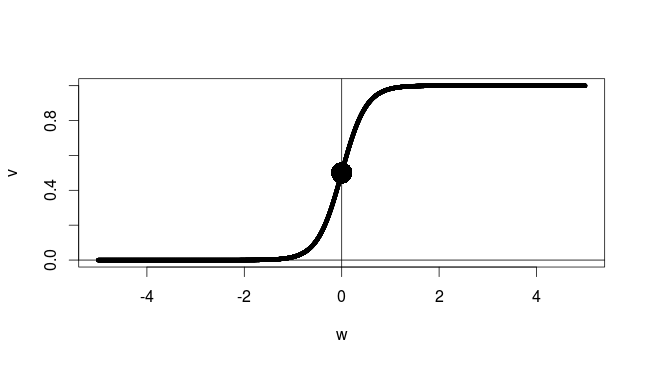
\includegraphics[width=6cm]{../fig/Cap13-CurvaLogistica1.png}
	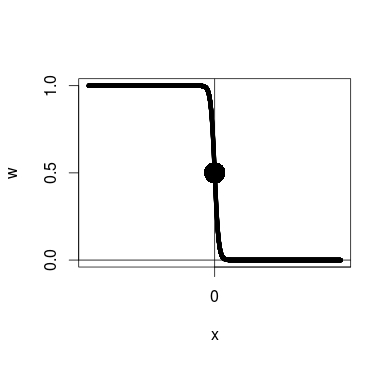
\includegraphics[width=6cm]{../fig/Cap13-CurvaLogistica2.png}\\
	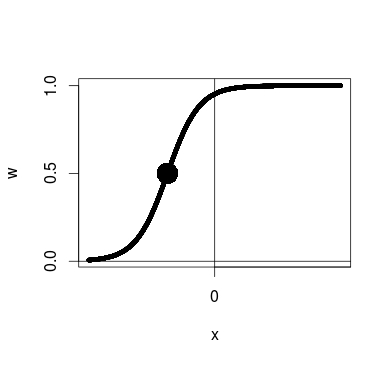
\includegraphics[width=6cm]{../fig/Cap13-CurvaLogistica3.png}
	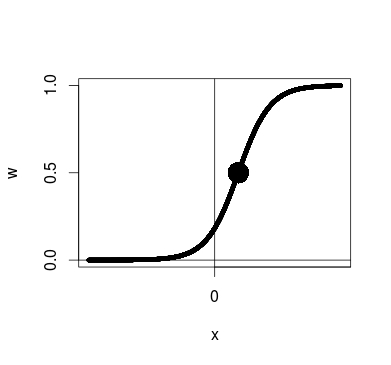
\includegraphics[width=6cm]{../fig/Cap13-CurvaLogistica4.png}
\caption{Curvas logísticas;
	arriba a la izquierda $w=e^{v}/(1+e^{v})$,
	arriba a la derecha $w=e^{-8v}/(1+e^{-8v})$,
	abajo a la izquierda $w=e^{3+v}/(1+e^{3+v})$,
	abajo a la derecha $w=e^{-1.5+v}/(1+e^{-1.5+v})$.
}
\label{cap13:fig:FiguraCurvaLogistica}
\end{center}
\end{figure}
\quad\\
\noindent Fíjate en que

\begin{itemize}

	\item En los gráficos superiores de la Figura \ref{cap13:fig:FiguraCurvaLogistica}, el signo de $b_1$ determina si $f$ crece (arriba a la izquierda, con $b_1>0$) o decrece (arriba a la derecha, con $b_1<0$). Además, cuanto mayor es (en valor absoluto) el coeficiente $b_1$, más brusca es la transición fracaso-éxito (o viceversa).   En particular, en el modelo que vamos a construir, el signo de $b_1$ está relacionado con el hecho de que la distribución de éxitos y fracasos sea directa ($b_1>0$) o inversa ($b_1<0$). Más adelante volveremos sobre el caso frontera $b_1 =0$.

	\item En los gráficos inferiores de la Figura \ref{cap13:fig:FiguraCurvaLogistica}	se muestra el efecto que tiene modificar el valor de $b_0$. Para mostrarlo, hemos tomado la curva de arriba a la izquierda, que tenía $b_0=0$ y $b_1=1$ y, manteniendo fijo el valor de $b_1$, hemos cambiado el valor de $b_0$. Como puedes ver, el efecto de $b_0$ es el de desplazar horizontalmente la curva, a la derecha, cuando $b_0<0$, o a la izquierda, cuando $b_0>0$.

	 \item En particular, cuando $b_0=0$, se cumple que $f(0)=1/2$. Es decir, el valor de la variable explicativa para el que las probabilidades de éxito y fracaso son la misma es $x=0$. Pero en ocasiones la variable explicativa (como el itb del Ejemplo  \ref{cap13:ejem:RegresionLogistica00}) no toma valores negativos, por lo que es necesario poder ``mover'' el punto de corte con el eje de ordenadas. Pero, como hemos visto, podemos elegir $b_0$ para obligar a $f(v)$ a cortar al eje de ordenadas en el punto $a\in(0,1)$ que queramos. Si queremos que ese punto de corte ocurra para un valor de $w=a$, una rápida manipulación algebraica muestra que, fijado $a\in(0,1)$, hay que elegir $b_0=\ln(a/(1-a))$.

	 \item Otro punto especialmente importante en esas gráficas es el punto
	 $$(x^*, f(x^*)=1/2).$$
	 Es decir, aquel en el que cambia la tendencia éxito-fracaso (o fracaso-éxito). En todas las curvas de la Figura \ref{cap13:fig:FiguraCurvaLogistica} lo hemos marcado con un ``punto gordo''.

\end{itemize}

La curvas logísticas son muy utilizadas en Ecología y en Bioquímica y, en ocasiones se denominan, directamente, como {\sf curvas con forma de S}\index{curva con forma de S} (en ingl\'es,  {\em S-shaped curves})\index{S-shaped curve} o {\sf curvas sigmoideas}\index{curva sigmoidea}. Recuerda, no obstante, que esa terminología es poco adecuada porque hay muchas otras clases de curvas sigmoideas, aparte de las curvas logísticas.


\subsubsection{Coeficientes y parámetros del modelo logístico.}
\label{cap13:subsubsec:CoeficientesParametrosModeloLogistico}

Las curvas logísticas van a ser, como hemos  dicho, un ingrediente esencial del  modelo que vamos a utilizar. El plan, recordémoslo, consiste en elegir los valores de $b_0$ y $b_1$ que proporcionan la mejor curva logística posible para nuestra muestra de puntos. Una vez que hayamos encontrado la mejor curva logística, la usaremos para hacer predicciones sobre las probabilidades, de manera que el valor de probabilidad predicho por el modelo será
  \begin{equation}\label{cap13:ec:logisticaEstimada}
    \hat{\pi}(x)=\dfrac{e^{b_0+b_1 x}}{1+e^{b_0+b_1 x}}.
  \end{equation}
Como antes,  el símbolo $\hat{\pi}$ representa el valor estimado, para distinguirlo del valor real (poblacional) $\pi(x)=P(Y=1|X=x)$ que hemos definido en la Ecuación \ref{cap13:ecu:ProbLogistica} (pág. \pageref{cap13:ecu:ProbLogistica}). Ya sabemos, por nuestra experiencia en capítulos anteriores, que al trabajar con una muestra lo que obtenemos son estimaciones. Esas estimaciones se corresponden con un modelo teórico en el que existen dos {\em parámetros} $\beta_0$ y $\beta_1$ tales que:
  \begin{equation}\label{cap13:ec:logisticaTeorica}
    \pi(x)=\dfrac{e^{\beta_0+\beta_1 x}}{1+e^{\beta_0+\beta_1 x}}.
  \end{equation}
Los {\em coeficientes} $b_0$ y $b_1$, que obtendremos para una muestra concreta, son estimadores de los parámetros teóricos $\beta_0$ y $\beta_1$, respectivamente.  En la próxima Sección \ref{cap13:sec:EstimacionParametros} vamos a abordar la cuestión de cómo encontrar los valores adecuados de $b_0$ y $b_1$. Una vez que hayamos hecho esto, nos detendremos a pensar un poco más sobre la interpretación de este modelo y sus posibles generalizaciones, tratando de aclarar en qué se parece y en qué es distinto de los modelos que hemos visto en anteriores capítulos.

\section{Estimaci\'on de los parámetros.}
\label{cap13:sec:EstimacionParametros}

Para echar a andar el modelo logístico, tenemos que afrontar la cuestión que hemos dejado pospuesta desde  la Sección \ref{cap13:sec:IntroduccionProblemaRegresionLogistica}. ¿Cuál es {\em ``la mejor curva logística''} posible, la que mejor se ajusta a la muestra? Concretando, eso quiere decir que tendremos que calcular los
dos coeficientes $b_0$ y $b_1$.

Recordemos que, en el contexto del modelo de regresión lineal simple, nuestra guía para encontrar los valores adecuados fue el criterio de minimizar el error cuadrático. Ese método tenía dos ventajas evidentes:
\begin{itemize}
  \item Una interpretación geométrica muy simple.
  \item El propio error cuadrático es uno de los términos que aparecen en la identidad Anova (ver la Ecuación \ref{cap10:ecu:AnovaparaRegresion}, pág. \pageref{cap10:ecu:AnovaparaRegresion})
\end{itemize}
Ahora, si tratamos de aplicar la misma idea, nos tropezamos con el hecho de que la propia estructura del modelo logístico hace que las dos ventajas queden neutralizadas (porque interviene $\pi(x)$ en lugar de $Y$ y porque, además, hacemos la transformación logit). Pero eso no quiere decir que no podríamos usar el método de mínimos cuadrados, basado en la técnica que vimos en la Sección \ref{cap13:subsec:AgrupandoValoresEstimarProbabilidades} (pág. \pageref{cap13:subsec:AgrupandoValoresEstimarProbabilidades}). Vamos a describir a continuación como se haría esto, pero queremos prevenir al lector de que {\bf esta no será la forma en la que, finalmente, construiremos los valores de $b_0$ y $b_1$ en el modelo de regresión logística.} Creemos que el riesgo de confusión que puede generar el ver dos formas distintas de proceder queda compensado por la ventaja de comprender que no hay un procedimiento único, y que cada uno tiene sus peculiaridades.

\subsection{Valores de $b_0$ y $b_1$  mediante mínimos cuadrados.}
\label{cap13:subsection:ParametrosCurvaSigmoideaMedianteMinimosCuadrados}
\noindent{\sc ADVERTENCIA:  ¡ESTO NO ES LA REGRESIÓN LOGÍSTICA!}

Para usar el método de mínimos cuadrados, una vez construidos como en la Sección \ref{cap13:subsec:AgrupandoValoresEstimarProbabilidades} (pág. \pageref{cap13:subsec:AgrupandoValoresEstimarProbabilidades}) los puntos
\[(w_1,\hat p_1),\ldots,(w_k,\hat p_k)\]
(recuerda que son los puntos triangulares rojos de la Figura \ref{cap13:fig:EjemploConstruccionModeloLogistico02}) basta con:
\begin{enumerate}
  \item Aplicar la transformación logit a los valores $\hat p_1,\ldots,\hat p_k$. Llamemos $l_1,\ldots,l_k$ a los valores resultantes. Este paso te recordará lo que hicimos en el Ejemplo \ref{cap10:ejem:RegresionNoLineal} (pág. \pageref{cap10:ejem:RegresionNoLineal}).
  \item Usando los métodos del Capítulo \ref{cap:RegresionLinealSimple} (mínimos cuadrados), calcular los coeficientes $\widetilde b_0$ y $\widetilde b_1$ de la recta de regresión
      \[l = \widetilde b_0 +\widetilde b_1\cdot w\]
      para los puntos
      \[(w_1,l_1),\ldots,(w_k,l_k).\]
      Hemos llamado $\widetilde b_0$ y $\widetilde b_1$ a los coeficientes porque, insistimos, el método que estamos exponiendo {\bf no} es el método que aplicaremos en la regresión logística. Y queremos usar símbolos distintos para los valores obtenidos por casa método.
  \item Construimos la curva logística correspondiente a esos valores $\widetilde b_0$ y $\widetilde b_1$.
\end{enumerate}

\begin{ejemplo}
\label{cap13:ejem:CurvaLogisticaPorMinimosCuadrados}
{\bf (Continuación del Ejemplo \ref{cap13:ejem:EstimacionModeloLogisticoMedianteClases}, pág. \pageref{cap13:ejem:EstimacionModeloLogisticoMedianteClases})}
Si aplicamos ese método a los datos del Ejemplo \ref{cap13:ejem:EstimacionModeloLogisticoMedianteClases}, se obtiene la curva de trazos azules de la Figura \ref{cap13:fig:EjemploModeloLogisticoMinimosCuadrados}, que corresponde a
\[\widetilde b_0\approx 0.1773,\qquad \widetilde b_1 = 0.9739\]

\begin{figure}[h!]
\begin{center}
\begin{enColor}
    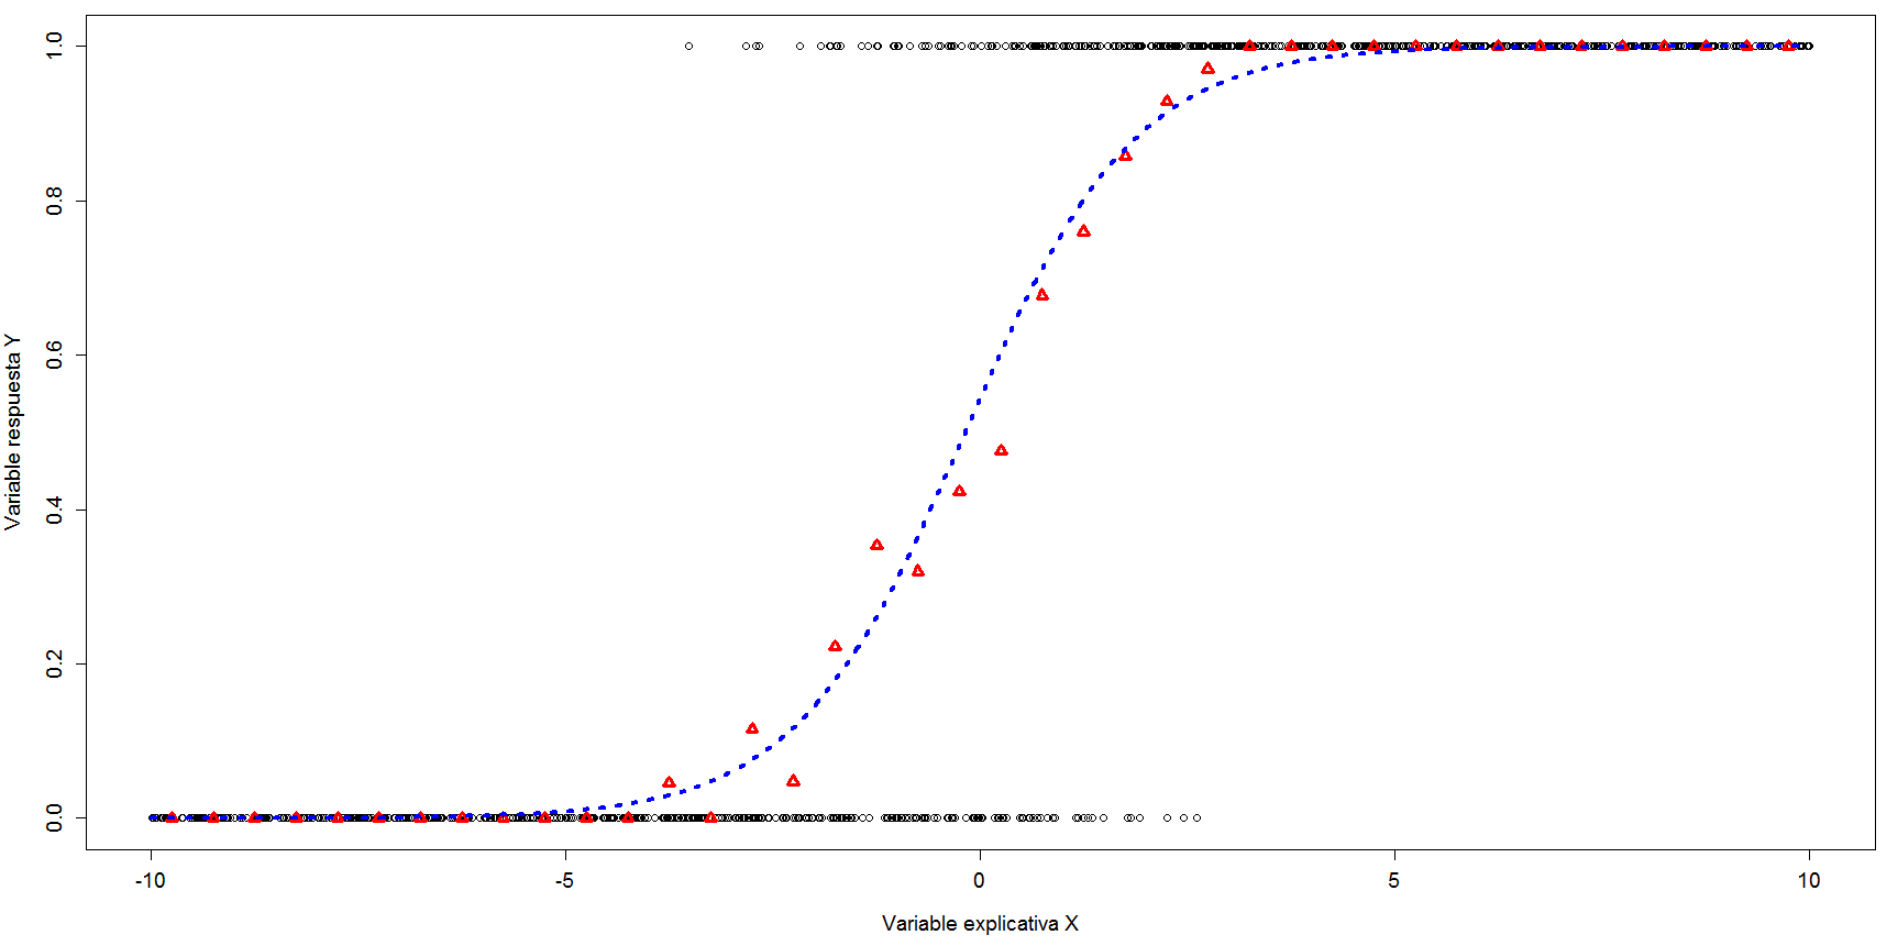
\includegraphics[width=13cm]{../fig/Cap13-EjemploModeloLogisticoMinimosCuadrados.png}
\end{enColor}
\begin{bn}
    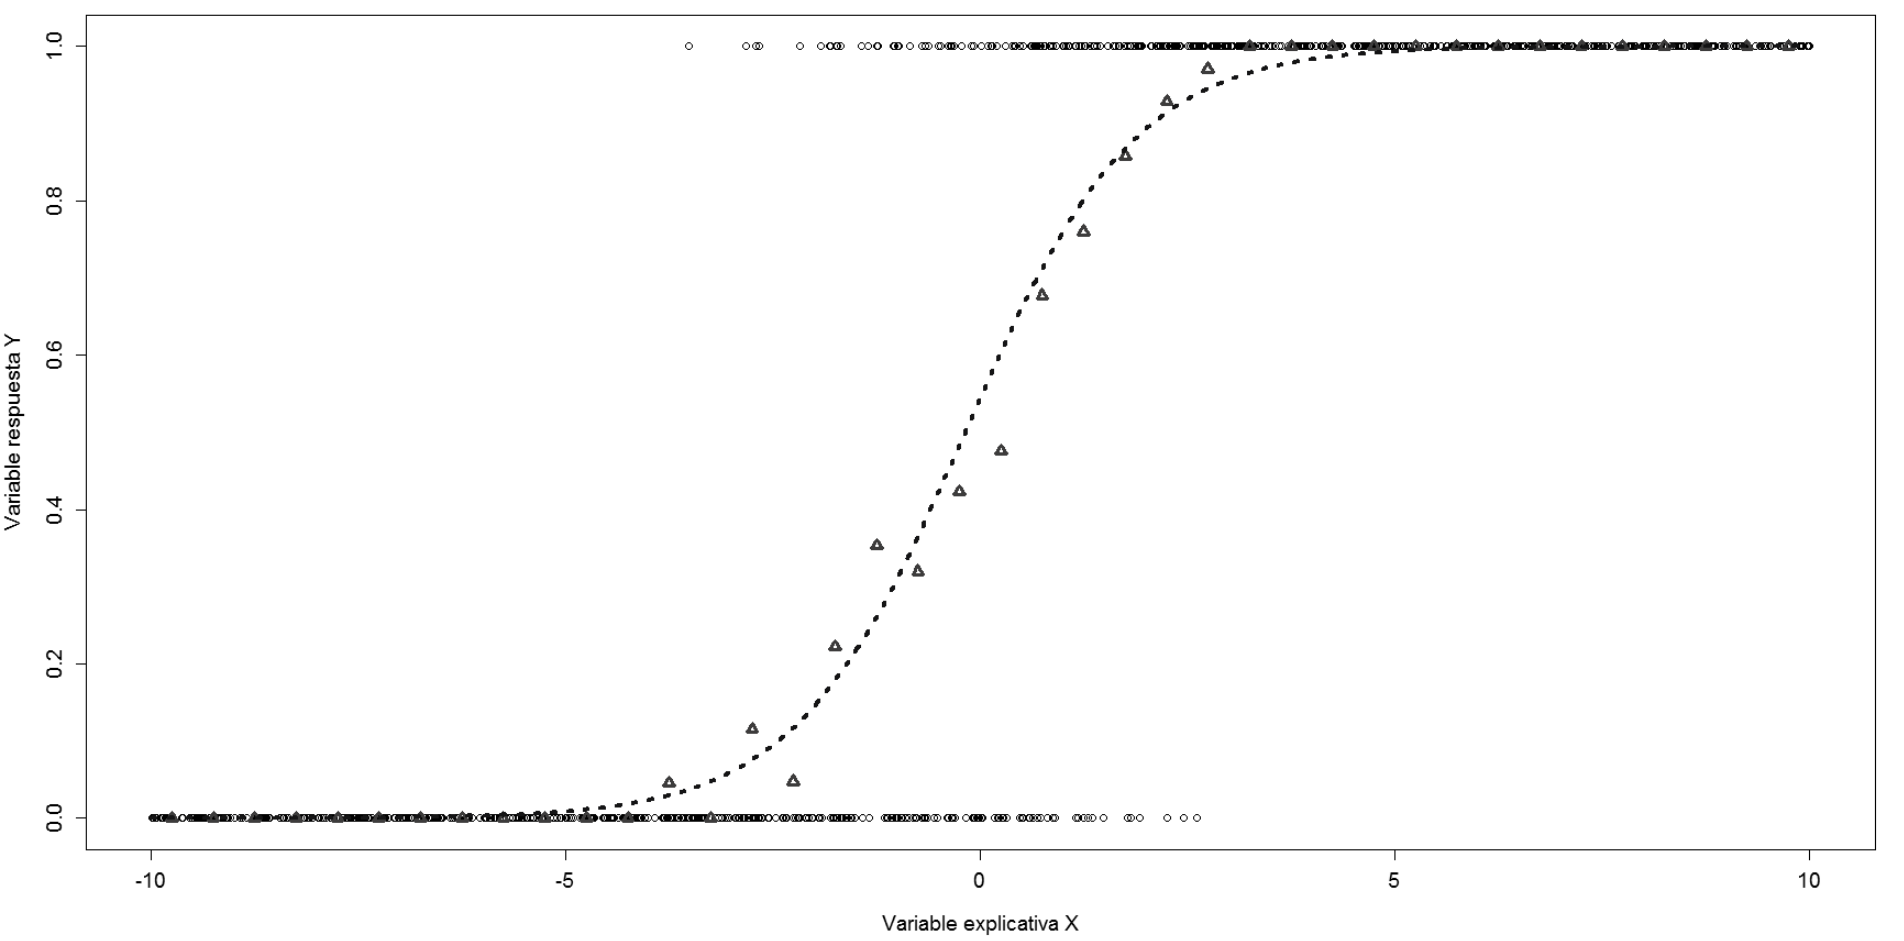
\includegraphics[width=13cm]{../fig/Cap13-EjemploModeloLogisticoMinimosCuadrados-bn.png}
\end{bn}
     \caption{Construcción, por el método de mínimos cuadrados, de una curva logística para los datos del Ejemplo \ref{cap13:ejem:EstimacionModeloLogisticoMedianteClases}. {!`}Esto no es regresión logística! }
     \label{cap13:fig:EjemploModeloLogisticoMinimosCuadrados}
\end{center}
\end{figure}

Como puedes ver en esa figura, el método proporciona una curva logística que parece hacer bastante bien el trabajo de aproximar las probabilidades $\hat p_i$. En el Tutorial13 veremos en detalle como aplicar el método para obtener esta curva.
\qed
\end{ejemplo}


\subsection{Regresión logística:  $b_0$ y $b_1$  mediante maxima verosimilitud.}
\label{cap13:subsection:ParametrosCurvaSigmoideaMedianteMaximaVerosimilitud}

El método que ilustra el anterior ejemplo se basa en la idea geométrica de minimizar los cuadrados de los residuos. En cambio, el modelo de regresión logística que se utiliza habitualmente se basa en el m\'etodo llamado {\sf método de máxima verosimilitud (MV)}\index{método de máxima verosimilitud (MV)}\index{verosimilitud} (en inglés, {\em maximum likelihood  method})\index{maximum likelihood method}\index{likelihood}. Recuerda que, en la Sección \ref{cap06:sec:MuestraAleatoriaSimpleFuncionVerosimilitud} (pág. \pageref{cap06:sec:MuestraAleatoriaSimpleFuncionVerosimilitud}) hemos definido la función de verosimilitud ${\cal L}(x_1,\ldots,x_n;\theta)$ de una muestra aleatoria simple, para una variable $X$ que depende de un parámetro $\theta$. Ahora, en realidad, estamos en una situación en la que tenemos dos parámetros $\beta_0$ y $\beta_1$ que estimar a partir de la muestra. Pero, salvo por eso, las ideas son muy similares.

Vamos a ver como se define la función de verosimilitud para este modelo. Quizá, para tener un punto de referencia y comparación,  quieras refrescar lo que aprendimos  sobre la  función de verosimilitud de una muestra aleatoria simple en la Ecuación \ref{cap04:ecu:FuncionVerosimilitudMuestraAleatoriaSimple} (pág. \pageref{cap04:ecu:FuncionVerosimilitudMuestraAleatoriaSimple}) y el Ejemplo \ref{cap06:ejem:FuncionDensidadConjuntaMuestraAleatoriaSimpleBernouilli-2} que seguía a esa ecuación.

En el ejemplo que nos ocupa ahora tenemos una muestra:
 \[(x_1, y_1), (x_2, y_2), \ldots, (x_n, y_n)\]
en la que la variable $Y$ sólo puede tomar los valores $0$ y $1$. Y hemos propuesto como modelo una curva logística que vincula los valores de $X$ con la probabilidad de que $Y$ tome el valor $1$:
\[
\hat{\pi}(x_i) = P(Y=1|X=x_i)= \dfrac{e^{b_0+b_1\cdot x_i}}{1+e^{b_0+b_1\cdot x_i}}.
\]
Utilizando ideas similares a las que vimos al obtener la Ecuación \ref{cap04:ecu:FuncionVerosimilitudMuestraAleatoriaSimple}  se puede ver que la función de verosimilitud en el caso que nos ocupa es:
\begin{equation}
\label{cap13:ecu:FuncionVerosimilitudLogistica}
{\cal L}(x_1,x_2,\ldots,x_n, y_1, y_2, \ldots, y_n;b_0, b_1) =\prod_{i:y_i=1}\hat{\pi}(x_i)  \cdot \prod_{i:y_i=0}(1 - \hat{\pi}(x_i)) =
\end{equation}
\[
=\prod_{i=1}^ n\hat{\pi}(x_i)^{y_i} \cdot (1 - \hat{\pi}(x_i))^{1 - y_i} =
\prod_{i:y_i=1} \dfrac{e^{b_0+b_1\cdot x_i}}{1+e^{b_0+b_1\cdot x_i}}
\cdot \prod_{i:y_i=0}\dfrac{1}{1+e^{b_0+b_1\cdot x_i}}
\]
En el segundo miembro de la primera línea, el primer factor contiene los términos correspondientes a los puntos $(x_i, 1)$ de la muestra y el segundo los  términos correspondientes a puntos $(x_i, 0)$.  La segunda línea comienza con una expresión alternativa de la función verosimilitud en forma de producto. Dejamos como ejercicio para el lector comprobar que las dos expresiones son equivalentes: sólo hay que recordar que los valores de $y_i$ sólo pueden ser uno o cero.

El resultado de este producto es una función complicada de las variables $b_0$ y $b_1$.  Y sobre esa función actúa el método de máxima verosimilitud. El objetivo del método es localizar los valores de $b_0$ y $b_1$ que producen un valor máximo de la verosimilitud.

\begin{ejemplo}
\label{cap06:ejem:FuncionMaximaVerosimilitud}
{\bf (Continuación del Ejemplo \ref{cap13:ejem:EstimacionModeloLogisticoMedianteClases}).}	
Para los datos del Ejemplo \ref{cap13:ejem:EstimacionModeloLogisticoMedianteClases} la función de verosimilitud  $\cal L$ tiene el aspecto que se muestra en la Figura \ref{cap06:fig:FuncionMaximaVerosimilitud}.  Veremos como dibujarla en el Tutorial13. Como puede apreciarse, existe una combinación de valores de $b_0$ y $b_1$ que produce un valor de la verosimilitud mayor que cualquier otro. Esos son precisamente los valores que el método va a  localizar. \qed

\begin{figure}[bth]
\begin{center}
\begin{enColor}
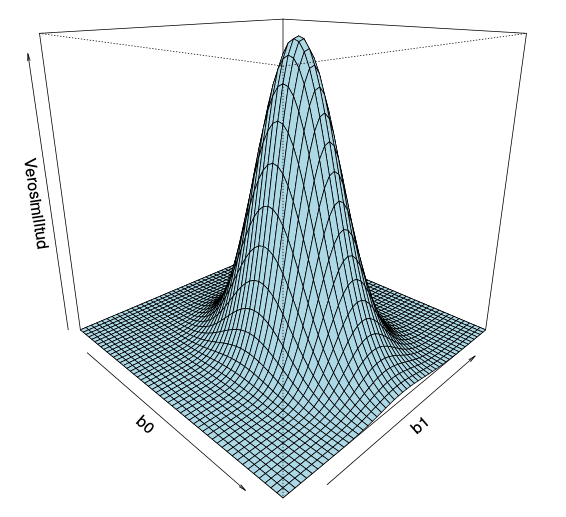
\includegraphics[width=8cm]{../fig/Cap13-EjemploFuncionVerosimilitud.png}
\end{enColor}
\begin{bn}
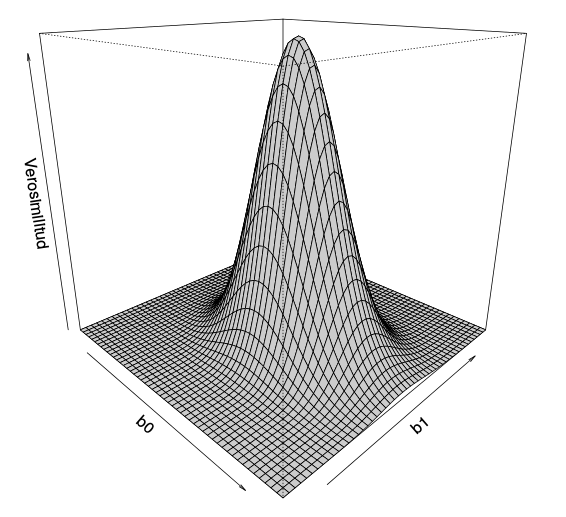
\includegraphics[width=8cm]{../fig/Cap13-EjemploFuncionVerosimilitud-bn.png}
\end{bn}
\caption{Función de máxima verosimilitud para los datos del Ejemplo \ref{cap13:ejem:EstimacionModeloLogisticoMedianteClases}.}
\label{cap06:fig:FuncionMaximaVerosimilitud}
\end{center}
\end{figure}
\end{ejemplo}

Como hicimos en el caso de la regresión lineal, no vamos a entrar en demasiados detalles sobre la descripción del método. Vamos a limitarnos a trazar un paralelismo con aquella otra situación conocida, la del modelo de regresión lineal simple. En aquel caso, se trataba de encontrar el valor mínimo del error cuadrático, visto como una función de los coeficientes $b_0$ y $b_1$. Recuerda el sistema de Ecuaciones \ref{cap10:ecu:SistemaDerivadasParcialesMinimosCuadrados} (pág. \pageref{cap10:ecu:SistemaDerivadasParcialesMinimosCuadrados}). En el caso de la regresión logística, el sistema análogo sería:
\begin{equation}
\label{cap10:ecu:SistemaDerivadasParcialesMaximaVerosimilitud}
\begin{cases}
\dfrac{\partial {\cal L}(b_0,b_1)}{\partial b_0}=0\\[3mm]
\dfrac{\partial {\cal L}(b_0,b_1)}{\partial b_1}=0
\end{cases}
\end{equation}
y lo que se busca son los valores de $b_0$ y $b_1$ que {\em maximizan} esa función de verosimilitud.

En realidad, se suele usar $-\ln({\cal L})$ y lo que se busca son los mínimos de esta función). La razón es que la verosimilitud de una muestra aleatoria simple es un producto. Además el logaritmo transforma productos en sumas y, para finalizar, la derivada de una suma es mucho más sencilla que la derivada de un producto. Todas esas razones justifican el uso frecuente del logaritmo de la verosimilitud. No vamos a hacer aquí el cálculo, para no alargar demasiado la discusión y no desalentar a los lectores menos experimentados con el Cálculo Diferencial.  El lector interesado encontrará todos los detalles en el Capítulo 7 de la referencia \cite{dobson2011introduction}.


%pero podemos mostrar al lector al menos los pasos iniciales cuando aplicamos esas ideas a la función verosimilitud de la Ecuación \ref{cap04:ecu:FuncionVerosimilitudMuestraAleatoriaSimple} (pág. \pageref{cap04:ecu:FuncionVerosimilitudMuestraAleatoriaSimple}). Concretamente, usando la expresión de $\cal L$ que aparece  al comienzo de la segunda fila de esa ecuación podemos escribir:
%\[
%\ln({\cal L})(x_1,x_2,\ldots,x_n, y_1, y_2, \ldots, y_n;b_0, b_1) =
%\sum_{i=1}^ n \bigl( {y_i} \ln(\hat{\pi}(x_i))  +  (1 - y_i) \ln(1 - \hat{\pi}(x_i)) \bigr)
%\]
%Y a partir de aquí las derivadas parciales son fáciles de obtener (conviene empezar )

Y además, afortunadamente, no es necesario que hagamos el trabajo duro a mano porque, al igual que en el caso del modelo de regresión lineal simple, cualquier programa estadístico que se precie de serlo hará por nosotros el cálculo de cuáles son los valores adecuados de los coeficientes. Un cálculo que será aproximado pero suficiente para nuestros propósitos.  En el  Tutorial13 veremos varios ejemplos. Es habitual utilizar el acento circunflejo para denotar que un parámetro ha sido estimado por este método de máxima verosimilitud, por lo que llamaremos $\hat{b}_0$ y $\hat{b}_1$, respectivamente, a los valores de $b_0$ y $b_1$ que nos proporciona el método.

\begin{ejemplo}
\label{cap13:ejem:CurvaLogisticaPorDosMetodos}
{\bf (Continuación del Ejemplo \ref{cap13:ejem:CurvaLogisticaPorMinimosCuadrados}).}
Si, usando el ordenador, obtenemos los valores $b_0$ y $b_1$ por el método de máxima verosimilitud para los datos del Ejemplo \ref{cap13:ejem:EstimacionModeloLogisticoMedianteClases}, obtendremos otra curva logística, distinta de la que obtuvimos en el Ejemplo \ref{cap13:ejem:CurvaLogisticaPorMinimosCuadrados}. Concretamente, allí teníamos
\[\widetilde b_0\approx 0.1773,\qquad \widetilde b_1 = 0.9739\]
mientras que para la curva de regresión logística se obtiene:
\[
\hat b_0 \approx 0.09526, \hat b_1 = 1.070
\]
En la Figura \ref{cap13:fig:CurvaLogisticaPorDosMetodos} pueden verse, juntas, ambas curvas logísticas.

\begin{figure}[h!]
\begin{center}
\begin{enColor}
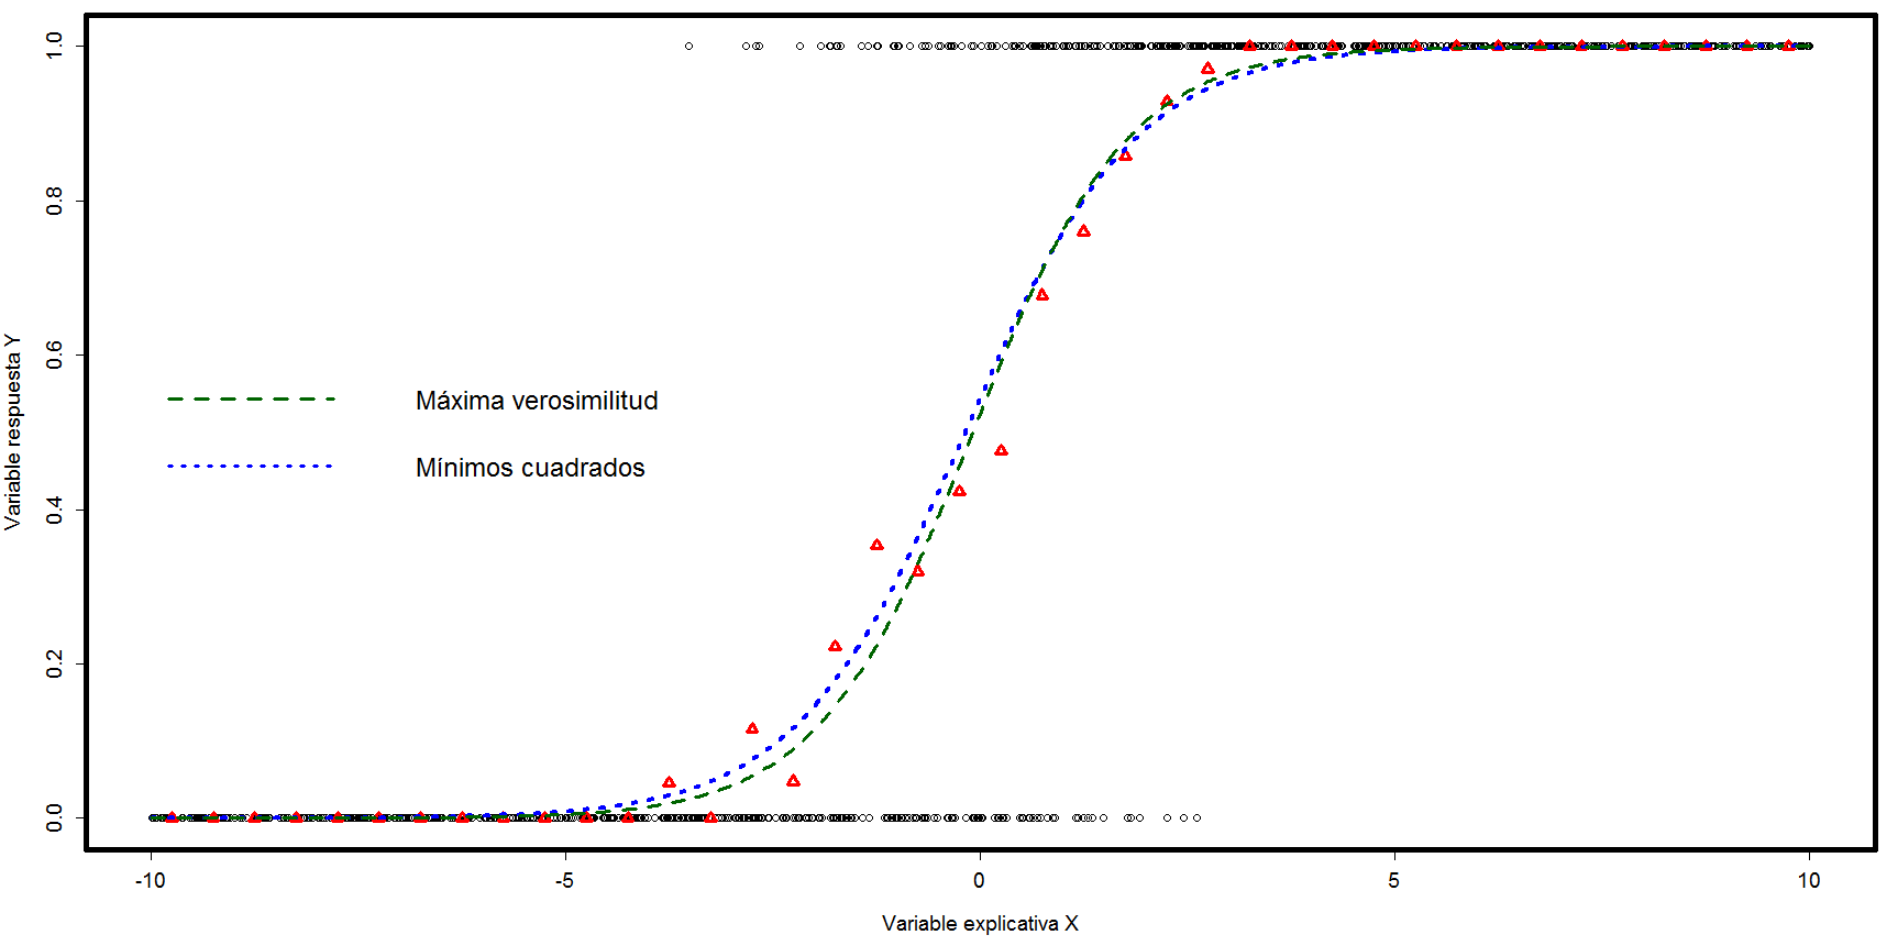
\includegraphics[width=13cm]{../fig/Cap13-CurvaLogisticaPorDosMetodos.png}
\end{enColor}
\begin{bn}
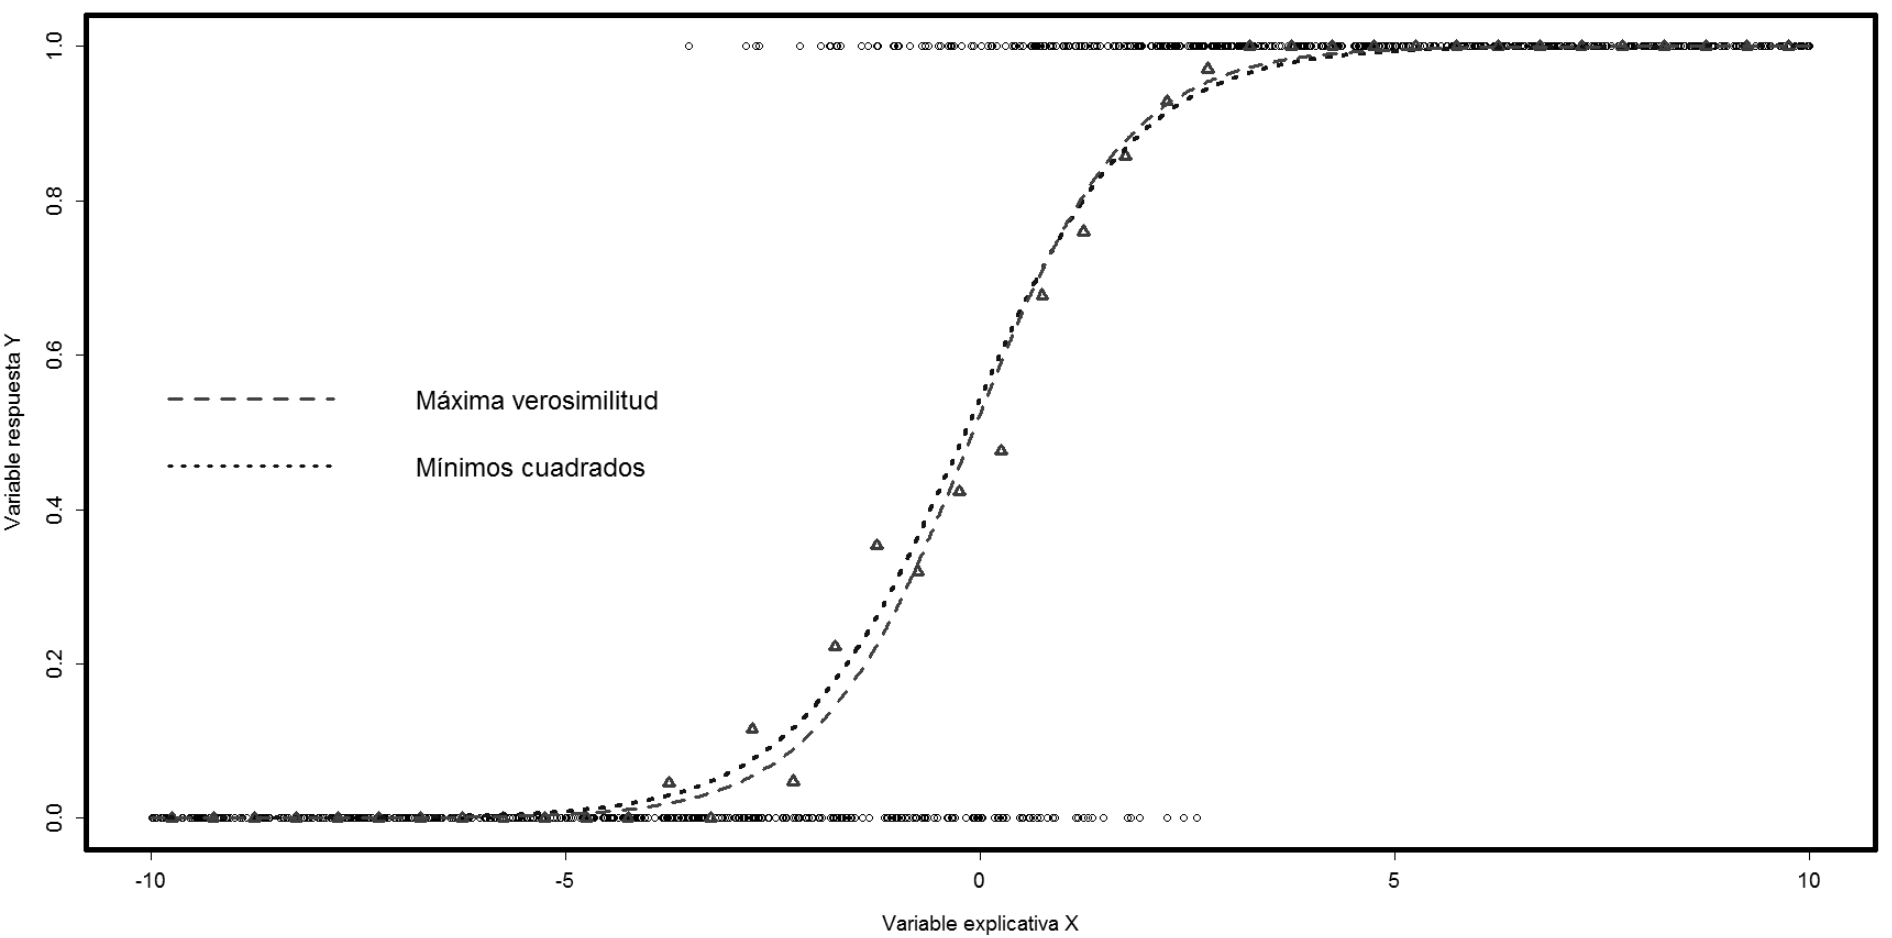
\includegraphics[width=13cm]{../fig/Cap13-CurvaLogisticaPorDosMetodos-bn.png}
\end{bn}
 \caption{Las curvas logísticas obtenidas por el método de mínimos cuadrados (puntos, color azul) y por el método de máxima verosimilitud (trazos verdes), para los datos del Ejemplo \ref{cap13:ejem:EstimacionModeloLogisticoMedianteClases}. }
 \label{cap13:fig:CurvaLogisticaPorDosMetodos}
\end{center}
\end{figure}
Como puedes comprobar, las dos curvas proporcionan buenas descripciones de los datos pero, desde luego, no coinciden. La curva obtenida por máxima verosimilitud es la del modelo de regresión logística. Hemos querido mostrar este ejemplo para ilustrar un punto que creemos que, por sutil, puede pasar desapercibido. Los datos son los mismos, y las dos curvas que aparecen son curvas logísticas, ajustadas ambas a esos datos por un modelo de regresión. Pero sólo una de ellas es realmente una curva de regresión logística.
\qed
\end{ejemplo}
Como trata de poner de manifiesto este ejemplo, no es el uso de curvas logísticas, por sí mismo, lo que define a la regresión logística. Además, es esencial tener en cuenta que los valores de los coeficientes se han determinado por el método de máxima verosimilitud, a partir de la función de verosimilitud que aparece en la Ecuación \ref{cap13:ecu:FuncionVerosimilitudLogistica} y que, a su vez, se basa en suponer que la distribución de las variables
\[
Y_i = Y|_{X=x_i}
\]
es en todos los casos una variable de tipo Bernoulli cuya probabilidad de éxito es $\hat{\pi}(x_i)$.  El uso de esa función verosimilitud y del  método de máxima verosimilitud para calcular los valores de $b_0$ y $b_1$ determina la estructura de error, o ruido, que acompaña al modelo. Y, como ya hemos visto, la esencia de un modelo estadístico depende de la adecuada combinación modelo/ruido.  %A esto es a lo que nos referíamos cuando dijimos, tras la Ecuación \ref{cap13:ecu:EcuacionGlm} (pág. \pageref{cap13:ecu:EcuacionGlm}) que la descripción del modelo lineal generalizado no estaba completa si sólo proporcionamos su función de enlace. Es necesario además describir las distribuciones de probabilidad de las respuestas  $Y_i$, que determinan la forma de $\cal L$.

La situación es similar a la que nos encontramos en el Capítulo \ref{cap:RegresionLinealSimple} (ver la Sección \ref{cap10:subsec:RegresionOrtogonal}, pág. \pageref{cap10:subsec:RegresionOrtogonal}) cuando hablamos de regresión ortogonal. Allí vimos que, dada una muestra de puntos $(x_i, y_i)$, había más de una forma de definir ``la mejor recta posible'' para aproximar esa muestra. Es muy importante, para llegar a entender los modelos lineales generalizados, comprender que, en los distintos métodos que vimos en el Capítulo \ref{cap:RegresionLinealSimple}, la muestra era todo el rato la misma, y en todos los casos usábamos rectas. Aquí, de nuevo, en el Ejemplo \ref{cap13:ejem:CurvaLogisticaPorDosMetodos} la muestra es la misma, y   las dos curvas que usamos son ambas curvas logísticas. Pero sólo una de ellas se ha obtenido por regresión logística. ¿Qué es lo que diferencia ambos métodos? La diferencia está en el método que utilizamos para el control del error. La ``mejor curva'' o la ``mejor recta'' son expresiones que sólo tienen sentido una vez que se ha definido el criterio por el que una curva (o recta) es mejor que otra. Y ese criterio consiste, siempre, en una descripción de cuál es el error que se desea minimizar. En el caso de la regresión lineal simple del Capítulo \ref{cap:RegresionLinealSimple}, la ```mejor recta'' era la recta que minimizaba el error cuadrático $EC$ (ver la página \pageref{cap10:ecu:RectaRegresionFormaPuntoPendiente}, en la que se definía la recta de regresión para el método de mínimos cuadrados). En aquel mismo capítulo, la recta de regresión ortogonal es la que minimiza la suma de cuadrados de las distancias de los puntos de la muestra a la recta. Y en el Ejemplo \ref{cap13:ejem:CurvaLogisticaPorMinimosCuadrados} hemos obtenido la curva logística que minimiza un cierto tipo de error cuadrático, como hemos explicado allí. Y entonces, ¿qué sucede en la regresión logística y en los modelos lineales generalizados? ¿Cuál es el criterio que se usa? En esos métodos usamos la curva que produce el máximo valor de la función de verosimilitud. Si te preocupa que aquí sea un {\em máximo}, mientras que en los demás casos era un {\em mínimo}, ten en cuenta que se trata de un matiz matemático, sin demasiada trascendencia: con cambiarle el signo a una función, los máximos se convierten en mínimos y viceversa. Y, de hecho, los máximos de la función verosimilitud ${\cal L}$ se suelen localizar, en la práctica, buscando cuáles son los mínimos de $-\ln({\cal L})$. Los dos problemas son, a todos los efectos, equivalentes.

\begin{ejemplo}
\label{cap13:ejem:coeficientesLogisticaVasculopatia}
Si aplicamos el método de máxima verosimilitud a los datos del Ejemplo \ref{cap13:ejem:RegresionLogistica00} (pág. \pageref{cap13:ejem:RegresionLogistica00}) sobre la relación entre el índice itb y la vasculopatía, se obtienen estos valores para los coeficientes:
\[
b_0 \approx 29.98, \qquad b_1 \approx -33.13
\]
La curva logística correspondiente a esos puntos, junto con el diagrama de dispersión original, aparece en la Figura \ref{cap13:fig:CurvaLogisticaVasculopatia}.

\begin{figure}[h!]
\begin{center}
\begin{enColor}
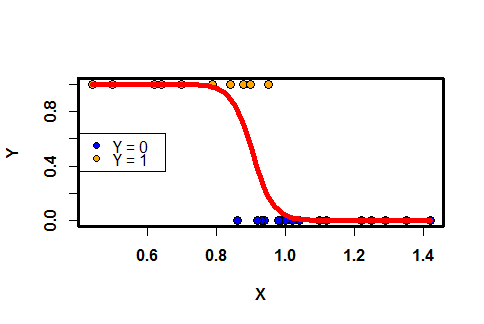
\includegraphics[width=11cm]{../fig/Cap13-CurvaLogisticaVasculopatia.png}
\end{enColor}
\begin{bn}
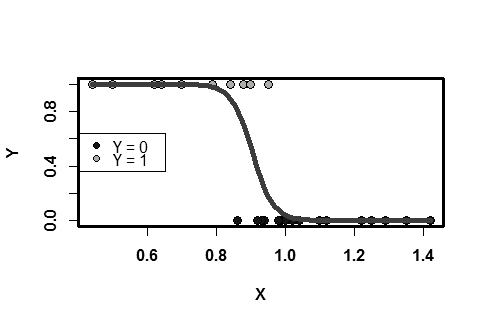
\includegraphics[width=11cm]{../fig/Cap13-CurvaLogisticaVasculopatia-bn.png}
\end{bn}
\caption{Curva logística para los datos itb / vasculopatía, en el
Ejemplo \ref{cap13:ejem:coeficientesLogisticaVasculopatia}. }
\label{cap13:fig:CurvaLogisticaVasculopatia}
\end{center}
\end{figure}
\qed
\end{ejemplo}



%\pendiente{\LARGE \textcolor{red}{ESTOY AQUÍ} }
%
%
%
%
%Veamos otro ejemplo de regresión logística, con los datos sobre vasculopatía y el índice itb.
%\begin{Ejemplo}\label{cap13:ContinuaEjemploRegresionLogistica} 	
%{\bf (Continuación del Ejemplo \ref{cap13:ejem:RegresionLogistica00}, pág \pageref{cap13:ejem:RegresionLogistica00}).}
%Usando el software adecuado, y a partir de los datos contenidos en la Tabla \ref{cap13:TablaDatosVasculopatia} (pág \pageref{cap13:TablaDatosVasculopatia}), hemos obtenido
%		$$\hat{b}_0=56.84\qquad\qquad\hat{b}_1=-61.66$$
%de donde tenemos
%	\begin{equation}\label{cap13:vasculopatiacurva}
%	\pi(x)=\dfrac{e^{ 56.84-61.66 x}}{1+e^{ 56.84-61.66x}}
%	\end{equation}
%que, en términos del logit, sería,
%	\begin{equation*}%\label{cap13:vasculopatiacurva}
%	g(x)=56.84-61.66 x.
%	\end{equation*}
%En la Figura \ref{cap13:Vasculopatialogistica} (pág \pageref{cap13:Vasculopatialogistica}) se representa la nube de puntos junto con la curva log\'istica 	que acabamos de fabricar.
%    \begin{figure}[h!]
%	\begin{center}
%        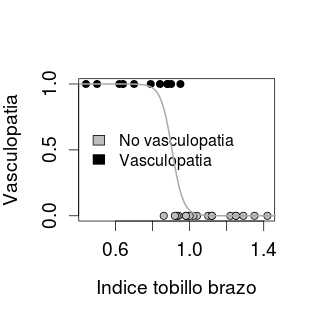
\includegraphics[width=8cm,height=8cm]{../fig/Cap13-VasculopatiaConCurvaLogistica.png}
%         \caption{Nube de puntos relativa al Ejemplo  \ref{cap13:ejem:RegresionLogistica00}
%         (pág \pageref{cap13:ejem:RegresionLogistica00}) junto con la curva 	
%         log\'istica ajustada con R mediante la funci\'on glm.} \label{cap13:Vasculopatialogistica}
%   \end{center}
%    \end{figure}
%La fórmula \eqref{cap13:vasculopatiacurva} asocia a cada valor del itb la probabilidad de desarrollar una vasculopat\'ia en el futuro, calculado a partir del valor del itb observado ahora. \qed
%\end{Ejemplo}


\section{Interpretación de los coeficientes de la curva logística.}
\label{cap13:sec:CurvasLogisticasPosibilidadesLogit}

En el modelo de regresión lineal simple del Capítulo \ref{cap:RegresionLinealSimple}, cuando pensábamos en la recta que define el modelo:
\[y = b_0 + b_1\cdot x\]
era fácil interpretar los coeficientes $b_0$ y $b_1$. Son, respectivamente, la ordenada en el origen y la pendiente de la recta, con significados geométricos muy intuitivos (ver el principio de la Sección \ref{cap10:sec:RectaRegresionECCorrelacion}, pág. \pageref{cap10:sec:RectaRegresionECCorrelacion}). En el modelo de regresión logística $b_0$ y $b_1$ tienen también, como hemos visto, una interpretación geométrica sencilla en relación con la forma de la curva logística. Pero, además, como vamos a ver, la propia estructura de esas curvas logísticas permite interpretar fácilmente esos coeficientes en términos de posibilidades (odds). Esta interpretación resulta especialmente útil en las aplicaciones del modelo logístico, por ejemplo en Epidemiología, que es uno de los campos científicos donde originalmente se desarrolló y aplicó este modelo.


\subsection{Transformación logit y posibilidades (odds).}

Hemos presentado la familia de curvas logísticas diciendo simplemente que se trata de curvas sigmoideas suficientemente sencillas. Y así es, desde luego. Pero hay algunas razones adicionales para pensar que esas curvas pueden ser una buena elección para el modelo que vamos a construir. Y por eso, antes de seguir adelante, vamos a detenernos un momento a discutir esas razones.

El enfoque que vamos a presentar enlaza directamente con el concepto de posibilidades (odds), que hemos encontrado ya varias veces en el curso. Concretamente, en las Secciones \ref{cap03:sec:OddsPruebasDiagnosticas} (pág.  \pageref{cap03:sec:OddsPruebasDiagnosticas})  y \ref{cap09:sec:RiesgoRelativoCocienteProbabilidades} (pág.  \pageref{cap09:sec:RiesgoRelativoCocienteProbabilidades}). Si aún no las has leído, este es un buen momento para hacerlo.

Para empezar, podemos volver a la Ecuación \ref{cap13:ec:logisticaEstimada} (pág. \pageref{cap13:ec:logisticaEstimada})
    \[\hat\pi(x)=\dfrac{e^{b_0+b_1\cdot x}}{1+e^{b_0+b_1\cdot x}},\]
Vamos a ir haciendo una serie de sustituciones, para poder interpretar de otra manera los ingredientes que aparecen en ella. Para empezar simplificando, llamaremos
\[s = b_0 + b_1\cdot x,\]
de manera que la Ecuación \ref{cap13:ec:logisticaEstimada} se traduce en
\[\hat\pi(x)=\dfrac{e^{s}}{1+e^{s}}.\]
Si, en esta ecuación, hacemos la sustitución
    \[ O = e^s,\]
(la elección de la letra $O$ no es casual, como veremos enseguida), se obtiene:
    \begin{equation}
    \label{cap13:ecu:RelacionPiConOdds}
        \hat\pi(x)=\dfrac{O}{1+O}.
    \end{equation}
Si, además, para recordar que $\hat\pi$ es una estimación de probabilidad, hacemos
    \[p=\hat\pi(x),\]
tendremos:
    \[p=\dfrac{O}{1 + O}.\]
A lo mejor, a primera vista, esta ecuación no te dice nada. Pero para quienes están familiarizados con la noción de posibilidades (odds), es evidente su relación con la Ecuación \ref{cap03:ecu:ProbabilidadesEnFuncionOdds} (pág. \pageref{cap03:ecu:ProbabilidadesEnFuncionOdds}), que relaciona posibilidades con probabilidades. A la luz de esa ecuación, está claro que lo que aquí hemos llamado $O$ juega el papel de posibilidades asociadas con la probabilidad $p$.  Y si, manteniendo esa idea en la cabeza, despejamos $s$ en función de $O$, tenemos
\begin{equation}
\label{cap13:ecu:RelacionPiConOdds02}
s= b_0+b_1\cdot x = \ln(O).
\end{equation}
Es decir, que estamos relacionando $b_0+b_1\cdot x$ con {\em el logaritmo de las posibilidades}. Y destacamos esto último, porque no es la primera vez que nos tropezamos con el logaritmo en relación con las posibilidades. Ya apareció en la Sección \ref{cap09:sec:RiesgoRelativoCocienteProbabilidades}, en la que argumentamos que el objetivo al tomar logaritmos era transformar unos intervalos en otros. Vamos a extendernos un poco más sobre esta interpretación, porque es la que permite una generalización muy interesante que desarrollaremos en el próximo apartado.

Para empezar, a partir de la Ecuación \ref{cap13:ecu:RelacionPiConOdds} y de la relación \ref{cap03:ecu:OddsEnFuncionProbabilidades} (pág. \pageref{cap03:ecu:OddsEnFuncionProbabilidades}), tenemos
\[
e^s = O = \dfrac{\hat\pi(x)}{1-\hat\pi(x)}.
\]
Y, por lo tanto, combinando esto con la Ecuación \ref{cap13:ecu:RelacionPiConOdds02}, se obtiene:
\begin{equation}
\label{cap13:ecu:RelacionPiConOdds03}
b_0+b_1\cdot x = \ln\left(\dfrac{\hat\pi(x)}{1-\hat\pi(x)}\right).
\end{equation}
En el modelo de regresión lineal simple tratábamos de ajustar la recta determinada por $b_0+b_1\cdot x$ a los valores de la variable respuesta $Y$. Aquí, como ya hemos discutido, lo que estamos tratando de predecir no son los valores de $Y$, sino las probabilidades asociadas $\hat\pi(x)$. Y, puesto que son probabilidades, son valores que viven en el intervalo $[0,1]$. Podemos pensar entonces en el miembro derecho de la Ecuación \ref{cap13:ecu:RelacionPiConOdds02} como una transformación de las probabilidades en dos etapas :
\begin{itemize}
  \item En la primera etapa, pasamos de probabilidades a posibilidades (odds):
        \[
        \hat\pi(x) \longrightarrow O=\dfrac{\hat\pi(x)}{1-\hat\pi(x)}
        \]
        Geométricamente, esta primera transformaci\'on lleva el intervalo $[0,1)$ al intervalo $[0,\infty)$, como ilustra la Figura \ref{cap12:Fig:OddsVsProbabilidad} (pág.  \pageref{cap12:Fig:OddsVsProbabilidad}).
  \item En la segunda etapa,
        \[
        O \longrightarrow \ln(O)
        \]
        el logaritmo transforma el intervalo $(0,+\infty)$ en el intervalo $(-\infty,+\infty)$ y, de esa forma, nos asegura que podamos usar una recta para ajustar los valores resultantes. Esta segunda transformación se ilustra en la Figura \ref{cap13:fig:GraficaLogaritmo} (pág. \pageref{cap13:fig:GraficaLogaritmo}).
\end{itemize}
Podemos argumentar así la necesidad de la segunda etapa: fíjate en que la ecuación $s=b_0 + b_1 \cdot x$ significa que la relación entre $x$ y $s$ se puede representar mediante una recta, en la que $b_0, b_1$ son la ordenada en el origen y la pendiente, respectivamente. En principio, al aplicar el modelo no hay ninguna restricción sobre los valores que puede tomar $x$. Y cuando $x$ varía de $-\infty$ a $\infty$, los valores de $b_0 + b_1 x$ también recorren todo el intervalo $(-\infty, \infty)$ (salvo en el caso especial $b_1=0$). Así que si queremos un modelo general, capaz de responder a cualquier conjunto de valores iniciales, debemos incluir el logaritmo en la segunda etapa, para tener cubiertos todos los valores de  $(-\infty, \infty)$.

\begin{figure}[bth]
\begin{center}
\begin{enColor}
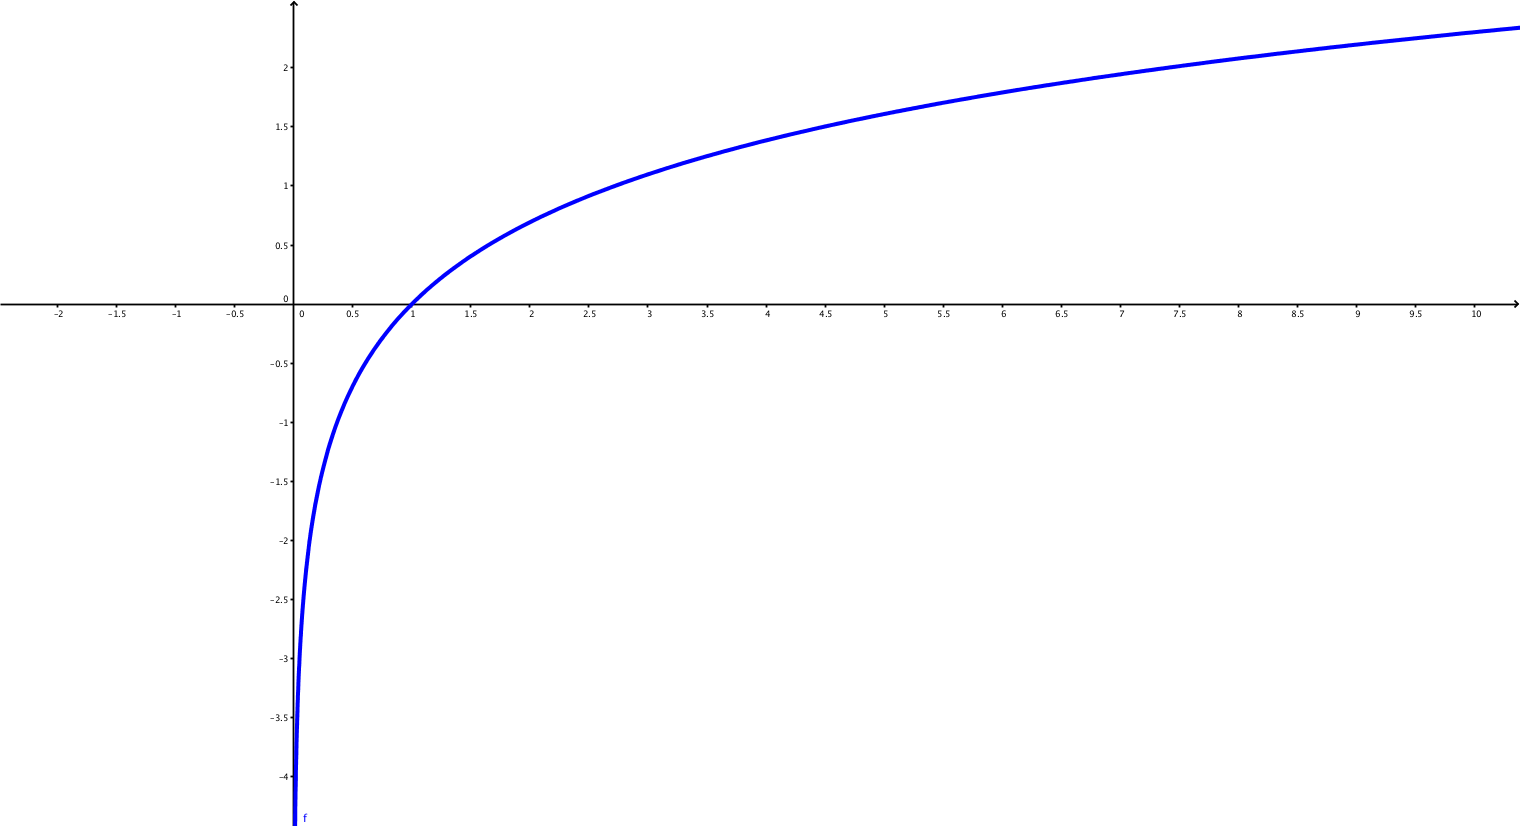
\includegraphics[width=13cm]{../fig/Cap13-GraficaLogaritmo.png}
\end{enColor}
\begin{bn}			
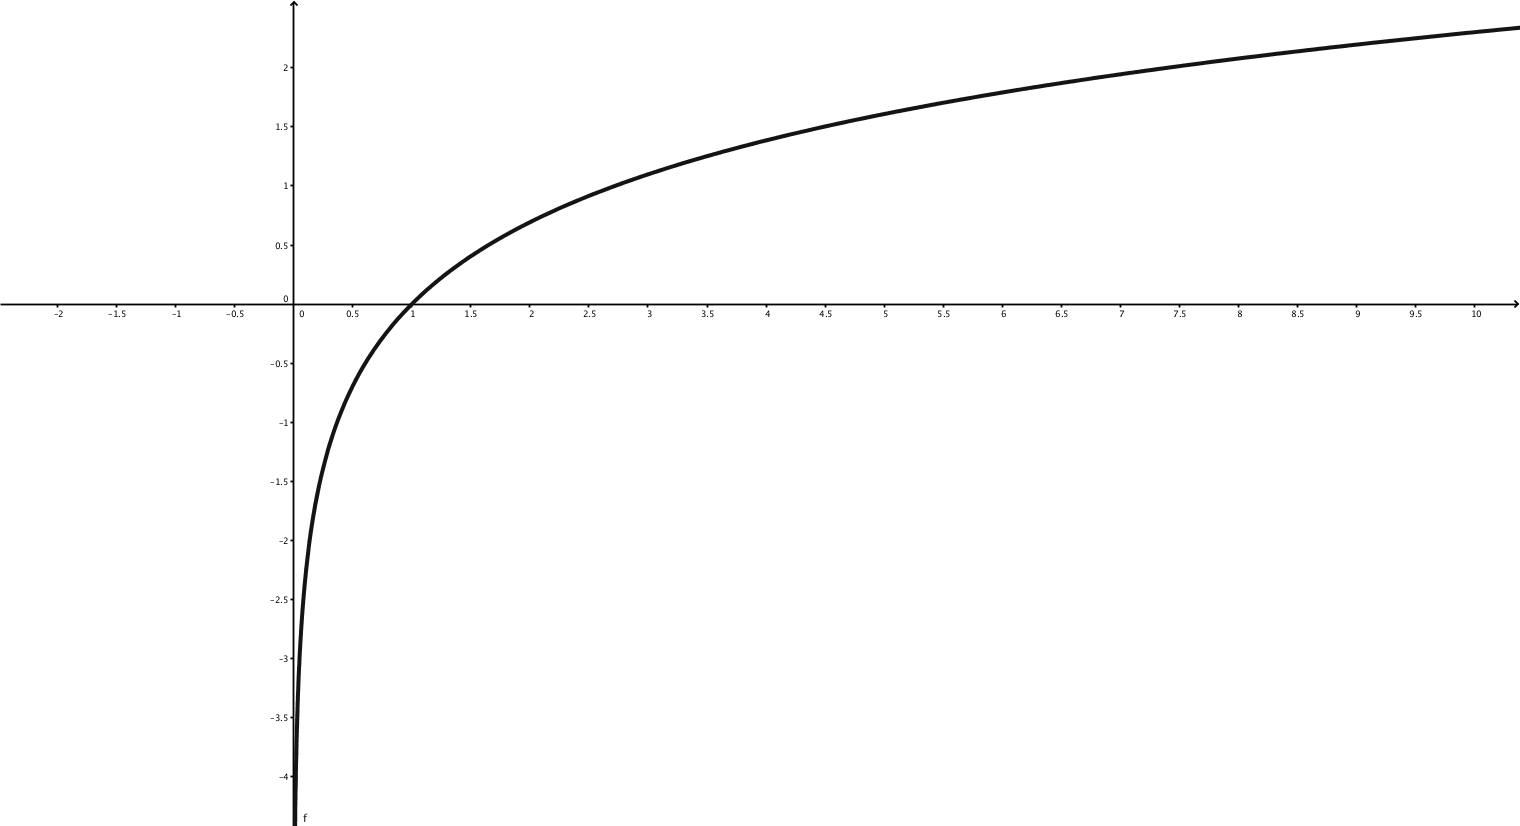
\includegraphics[width=13cm]{../fig/Cap13-GraficaLogaritmo-bn.png}
\end{bn}
\caption{Transformación del intervalo $(0, \infty)$ en el intervalo $(-\infty, \infty)$ mediante el logaritmo.}
\label{cap13:fig:GraficaLogaritmo}
\end{center}
\end{figure}

El resultado de concatenar (o {\em componer}, en el lenguaje de las matemáticas) las dos transformaciones correspondientes a esas dos etapas  es un proceso que asocia $\pi(x)$ con $\ln(\pi(x)/(1-\pi(x))$, y que se conoce como \textsf{transformación logit}\index{transformación logit}\index{logit}.
\begin{center}
    \fcolorbox{black}{Gris025}{
    \begin{minipage}{12cm}
        \begin{center}
        %%%%%%%%%%%%%%%%%%%%%%%%%%%%%%%%%%%%%%%
        {\bf  Transformación logit.}
        \end{center}
        %%%%%%%%%%%%%%%%%%%%%%%%%%%%%%%%%%%%%%%
        La {\sf transformación logit} convierte los valores del intervalo $(0,1)$ (normalmente, interpretados como probabilidades) en valores del intervalo $(-\infty,\infty)$, y se define mediante:
          \begin{equation}\label{cap13:ecu:TransformacionLogit}
        	p\longrightarrow \ln\left(\dfrac{p}{1-p}\right).
          \end{equation}
        %%%%%%%%%%%%%%%%%%%%%%%%%%%%%%%%%%%%%%%
    \end{minipage}}
    \end{center}
Como decíamos al principio de este apartado, esta interpretación de las curvas logísticas en términos del logaritmo de las posibilidades hace que la elección de esa familia de curvas, como base del modelo que vamos a construir, resulte algo menos artificial.

\subsection{Interpretaci\'on de los parámetros de la curva log\'istica.}
\label{cap13:subsection:interpretacionparametros}



%En el caso de la regresión logística, las transformaciones asociadas con ese modelo hacen que no nos sea posible dar una interpretaci\'on geométrica sencilla de los parámetros. Pero eso no significa que no podamos interpretarlos de alguna otra forma, no geométrica.
Como vamos a ver, cada uno de los parámetros $\beta_0$ y $\beta_1$ tiene su propio significado en términos de
posibilidades (odds). Recuerda la relaci\'on
%\eqref{cap13:ec:logit}
\ref{cap13:ecu:RegresionLogisticaComoGlm} (pág. \pageref{cap13:ecu:RegresionLogisticaComoGlm}), que reproducimos a continuaci\'on:

\begin{equation*}
\ln\left(\dfrac{\pi(x)}{1-\pi(x)}\right)=\beta_0+\beta_1 x.
\tag{\ref{cap13:ecu:RegresionLogisticaComoGlm} repetida.}
\end{equation*}
Con esa relaci\'on en mente, $\beta_1$ da una medida de c\'omo var\'ia el logaritmo de
las posibilidades (odds) de $\pi(x)$ al aumentar $X$ una unidad desde el valor actual. Es decir,
para hacer la comparaci\'on restamos
	\[\ln\left(\dfrac{\pi(x+1)}{1-\pi(x+1)}\right)=\beta_0+\beta_1 (x+1)
	\qquad \text{y} 	\qquad \ln\left(\dfrac{\pi(x)}{1-\pi(x)}\right)=\beta_0+\beta_1 x \]
y obtenemos
	\[\ln\left(\dfrac{\pi(x+1)}{1-\pi(x+1)}\right)-\ln\left(\dfrac{\pi(x)}{1-\pi(x)}\right)=\beta_1 \]
Si tomamos exponenciales en esta igualdad, simplificamos y reordenamos, obtenemos
	\[e^{\beta_1}=\dfrac{\frac{\pi(x+1)}{1-\pi(x+1)}}{\frac{\pi(x)}{1-\pi(x)}}\]
esta expresi\'on es el cociente de posibilidades (odds ratio),
que introdujimos en la Secci\'on \ref{cap09:ecu:DefinicionOddsRatio}
(pág. \pageref{cap09:ecu:DefinicionOddsRatio}). En este contexto, se interpreta
como la proporci\'on entre las posibilidades (odds) esperadas de observar $Y=1$
cuando aumenta una unidad la variable explicativa. \newline

Por otro lado, para interpretar el parámetro $\beta_0$, tomamos exponenciales en
la Ecuación     \ref{cap13:ecu:RegresionLogisticaComoGlm} y tenemos
	\[e^{\beta_0}\cdot e^{\beta_1 x}=\dfrac{\pi(x)}{1-\pi(x)}.\]
Si hacemos $X=0$, resulta
	\[e^{\beta_0}=\dfrac{\pi(0)}{1-\pi(0)}\]
o, lo que es lo mismo, la exponencial de $\beta_0$ nos proporciona las  posibilidades (odds)
de un individuo para el que la variable explicativa vale $X=0$, cuando esto tenga sentido.
%
%
%Antes de usar la f\'ormula \eqref{cap13:vasculopatiacurva} para realizar predicciones, hay varios aspectos que es importante retener:
%	\begin{enumerate}	
%	\item Que seamos capaces de estimar unos valores $\hat{b}_0$ y $\hat{b}_1$ para los parámetros $b_0$ y $b_1$ no significa que, necesariamente, \emph{la} curva logística obtenida sea la adecuada
%	para nuestros propósitos. Sucede lo mismo que al hacer regresión lineal; piensa,
%	por ejemplo, en el cuarteto de Anscombe \ref{cap10:subsec:CuartetoAnscombe} (pág
%	\pageref{cap10:subsec:CuartetoAnscombe}). Por tanto, el primer paso es asegurar la
%	``calidad'' de los parámetros estimados. Y mediremos esto en términos de la
%	\emph{bondad} de la aproximación de las probabilidades predichas por el modelo
%	(la curva logística) a las probabilidades observadas. Compararemos
%	lo que predice el modelo con lo que quemos observado en la muestra y la
%	herramienta de medida adecuada son los contrastes $\chi^ 2$
%	que abordamos en el Cap\'itulo \ref{cap12:sec:ChiCuadradoHomgeneidad}.
%
%   	\item  A\'un en el supuesto de que el ajuste sea bueno, es de interés averiguar
%   	si la variable explicativa o no relevante para describir el comportamiento de la
%   	variable respuesta.  El análogo en
%	t\'erminos de un problema de regresi\'on lineal simple está en la Secci\'on
%	\ref{cap10:subsec:modeloRegresionLinealSimple} (en concreto, en la
%	pág.  \pageref{cap10:subsubsec:IntervaloConfianzaPendiente}).
%   	
%   	\item Y, finalmente, asignaremos una medida a lo valiosa que resulta esta curva log\'istica
%   	  en cuanto a predictor de las probabilidades de que $Y=1$.  C\'omo se desarrolla esta idea
%   	  no tiene parang\'on en el contexto de la regresi\'on lineal.
%	\end{enumerate}

\section{Modelos lineales generalizados y funciones de enlace}
\label{cap13:sec:FuncionesEnlace}

{\bf Advertencia: Para entender el contenido de esta sección es conveniente haber leído las Secciones \ref{cap10:sec:InferenciaRegresionLineal} (pág. \pageref{cap10:sec:InferenciaRegresionLineal}) y \ref{cap10:sec:ModelosDeRegresion} (pág. \pageref{cap10:sec:ModelosDeRegresion}) del Capítulo \ref{cap:RegresionLinealSimple}, junto con la Sección \ref{cap11:subsec:AnovaComoModeloLineal} (pág. \pageref{cap11:subsec:AnovaComoModeloLineal}) del Capítulo \ref{cap:IntroduccionAnova}.}


Vamos a aprovechar el trabajo de las anteriores secciones para tratar de situar de forma adecuada la regresión logística, en relación con los modelos que hemos visto en capítulos anteriores.

Es posible que la discusión de la anterior Sección \ref{cap13:sec:CurvasLogisticasPosibilidadesLogit} haya hecho recordar al lector lo que ya hicimos en la Sección \ref{cap10:sec:ModelosDeRegresion} (pág. \pageref{cap10:sec:ModelosDeRegresion}), cuando vimos que era posible extender el uso de la regresión lineal a otras situaciones mediante transformaciones de las variables. En particular, en el Ejemplo \ref{cap10:ejem:RegresionNoLineal} (pág. \pageref{cap10:ejem:RegresionNoLineal}) se analiza un problema en el que, en lugar de la variable original $Y$, ajustamos una recta a los valores del {\em logaritmo} de la variable $Y$.  Precisamente eso, el uso del logaritmo, es lo que tienen en común ambas situaciones. Y ese parecido superficial puede generar en el lector la confusión que ahora queremos tratar de evitar, porque hay una diferencia entre las dos situaciones que es mucho más profunda que lo que comparten. En aquel caso, en el Capítulo \ref{cap:RegresionLinealSimple}, los valores que transformábamos eran siempre los de la variable respuesta $Y$. Ahora, y es esencial recordarlo, los valores que tratamos de ajustar son los de la probabilidad (condicionada) $\pi(x)=P(Y|X=x)$.

En particular, ese hecho implica que el modelo de regresión logística no pertenece a la categoría de modelos lineales de los que hemos hablado en los Capítulos \ref{cap:RegresionLinealSimple} (Regresión lineal) y \ref{cap:IntroduccionAnova} (Anova). La regresión logística es el ejemplo más común, y el primero que nos encontramos, de los que se conocen como {\sf modelos lineales generalizados}\index{modelos lineales generalizados} (en inglés, {\em generalized linear models}, que muchas veces se abrevia en {\em glm}).\index{generalized linear models}\index{glm} El estudio detallado de los modelos lineales generalizados nos llevaría más allá del nivel introductorio que tratamos de mantener en este libro. Pero, como hemos hecho en otros casos, queremos ofrecer al lector al menos un punto de vista inicial sobre esos modelos, para que, cuando llegue a cursos más avanzados, el primer paso ya esté dado.

Como hemos dicho, el modelo de regresión logística trata de establecer una relación entre, por un lado un término de la forma $\beta_0+\beta_1\cdot x$ (como el de la regresión lineal) y, por otro lado, la transformación logit aplicada a la probabilidad condicionada:
\[\pi(x)=P(Y=1|X=x).\]
Esa relación viene dada por la versión teórica de la Ecuación \ref{cap13:ecu:RelacionPiConOdds03} (pág. \pageref{cap13:ecu:RelacionPiConOdds03}), que es:
\begin{equation}
\beta_0+\beta_1\cdot x = \ln\left(\dfrac{\pi(x)}{1-\pi(x)}\right).
\end{equation}
Para entender el punto de vista que se utiliza en los modelos lineales generalizados, tenemos que aprender a ver esta probabilidad condicionada de otra manera.

Recordemos que, en  lo que llevamos de este capítulo, hemos considerado siempre que la variable respuesta $Y$ sólo puede tomar los valores $0$ o $1$, como una variable de tipo $Bernouilli(p)$, en la que $\pi(x)$ hace el papel de la probabilidad de éxito $p$. Recuerda que la media o esperanza $\mu$ de una variable de tipo $Bernouilli(p)$ es precisamente igual a $p$ (ver la Ecuación \ref{cap05:ecu:MediaVariableBernouilli}, pág. \pageref{cap05:ecu:MediaVariableBernouilli}). Así que, si hasta ahora hemos estado pensando en $\pi(x)$ como una probabilidad, estas observaciones significan que también podemos pensar en $\pi(x)$ como la media de la variable condicionada $(Y|X=x)$ (ver la Sección \ref{cap04:sec:IndependenciaVariablesAleatoriasDiscretas}, en la que introdujimos la idea de distribuciones condicionadas):
\begin{equation}
\label{cap13:ecu:PiComoEsperanza}
\pi(x)=E(Y=1|X=x)=\mu_{Y|X=x}.
\end{equation}
Por lo demás, el modelo se interpreta exactamente igual, de manera que el objetivo es obtener el valor de $\mu_{Y|X=x}$ o, más precisamente, de su transformada logit, a partir del término $\beta_0+\beta_1\cdot x$. Es decir:
\begin{equation}
\label{cap13:ecu:RegresionLogisticaComoGlm}
\operatorname{logit}(\mu_{Y|X=x}) =
\ln\left(\dfrac{\mu_{Y|X=x}}{1-\mu_{Y|X=x}}\right)=
\beta_0+\beta_1\cdot x.
\end{equation}
Esto es importante, porque esa es la idea que lleva a los modelos lineales generalizados. Ya hemos visto que la transformación logit está relacionada con la familia de curvas logísticas. Y también sabemos que esas curvas logísticas son sólo una de las muchas familias de curvas sigmoideas con las que podríamos haber empezado a trabajar. Si hubiéramos utilizado otra familia, obtendríamos una transformación distinta del logit. Por ejemplo, cuando se usa la familia $\Phi_{\mu,\sigma}$ (funciones de distribución de variables normales), se obtiene una transformación distinta, llamada {\sf probit}\index{probit}.

Teniendo esto en cuenta, la definición de los modelos lineales generalizados es, esencialmente, la misma idea que ya hemos expuesto en la Ecuación \ref{cap13:ecu:RegresionLogisticaComoGlm}, pero permitiendo una transformación cualquiera, sin limitarnos a usar necesariamente logit.
\begin{center}
\fcolorbox{black}{Gris025}{
	\begin{minipage}{12cm}
	\begin{center}
	%%%%%%%%%%%%%%%%%%%%%%%%%%%%%%%%%%%%%%%
		{\bf  Modelo lineal generalizado (glm) y función de enlace.}
	\end{center}
	%%%%%%%%%%%%%%%%%%%%%%%%%%%%%%%%%%%%%%%
	Un modelo lineal generalizado entre la variable predictora $X$ y la variable respuesta $Y$ establece una relación de la forma
	\begin{equation}\label{cap13:ecu:EcuacionGlm}
		g(\mu_{Y|X=x}) = \beta_0+\beta_1\cdot x.
		\end{equation}
	donde $g$ es una transformación que recibe el nombre de {\sf función de enlace}\index{función de enlace (glm)}\index{enlace, función de (glm)} (en inglés, {\em link function}\index{link function (glm)}).\\
	{\bf Observación:} la Ecuación \ref{cap13:ecu:EcuacionGlm} no constituye una descripción completa del modelo lineal generalizado. Es, además, necesario conocer la distribución de la variable $Y$. Ver el Ejemplo \ref{cap13:ejem:CurvaLogisticaPorDosMetodos} (pág. \pageref{cap13:ejem:CurvaLogisticaPorDosMetodos}) y la discusión que lo acompaña para aclarar esto.
			%%%%%%%%%%%%%%%%%%%%%%%%%%%%%%%%%%%%%%%
		\end{minipage}}
	\end{center}
	
\noindent{\bf Observaciones:}
	
En la regresión logística, como hemos dicho, la función de enlace es el logit. Como hemos indicado, esta descripción del modelo no está realmente completa hasta que conocemos la distribución condicionada de la variable $Y|_{X=x}$, porque esa distribución es la que nos permite evaluar el comportamiento del modelo. Entender esto nos va costar algo de esfuerzo y, además, la discusión detallada queda fuera del nivel introductorio que estamos tratando de mantener. Pero podemos tratar de hacernos una idea de lo que sucede. A primera vista, la descripción del modelo que proporciona la Ecuación \ref{cap13:ecu:EcuacionGlm} parece muy distinta de las que hemos visto en el caso del modelos de regresión lineal simple, que era (ver la Ecuación \ref{cap10:ecu:InterpretacionModeloRegresionLinealSimple}, pág. \pageref{cap10:ecu:InterpretacionModeloRegresionLinealSimple}):
	\[
	y=
	\underbrace{\beta_0 +\beta_1\cdot x}_{\mbox{modelo}}
	+
	\underbrace{\phantom{\beta}\epsilon\phantom{\beta}}_{\mbox{ruido}},
	\quad\mbox{ siendo }\epsilon\sim N(0,\sigma).
	\]
	Para ver con más claridad la conexión entre las dos formas de describir un modelo, imagínate que fijamos el valor de $X=x$ en el modelo de regresión lineal simple. ¿Cuánto vale, en ese caso, el valor medio $\mu_{Y|X=x}$? Pues, teniendo en cuenta que el valor medio del término de error $\epsilon$ es $0$, se tiene:
	\[
	\mu_{Y|X=x} = \beta_0 +\beta_1\cdot x.
	\]
	Es decir, que el modelo de regresión lineal simple se puede ver como un modelo lineal generalizado, en el que la función de enlace es la identidad (la que deja el valor de $\mu$ intacto). Y, de paso, como decíamos, esto nos ayuda a ver que la Ecuación \ref{cap13:ecu:EcuacionGlm} se puede entender realmente como la descripción de un modelo que relaciona las variables $X$ e $Y$. Lo que no proporciona directamente esa ecuación es una  descripción del error asociado con este modelo, como la que teníamos en el modelo lineal. No vamos a entrar a fondo en los detalles técnicos de los modelos lineales generalizados, porque su lugar natural es un curso de Estadística más avanzado. Eso sí, un poco más adelante en esta misma sección vamos a dar algunas indicaciones (opcionales) sobre el error en la regresión logística y en los modelos lineales generalizados, confiando en que en el futuro el lector pueda usarlos para conseguir una transición más suave hacia la Estadística avanzada.  Lo importante es que el lector sea consciente de que con la regresión logística hemos salido del mundo de los modelos lineales y sus términos de error normales.
	
\subsubsection*{Variables dependientes dicotómicas y politómicas. Regresión multinomial.}
	\label{cap13:subsubsec:VariablesDicotomicasPolitomicasRegresionMultinomial}
	
	El matiz que queremos hacer aquí suele pasarse por alto, pero creemos que es {\bf extremadamente importante} para que el lector se haga una composición de lugar correcta de cuáles son las técnicas adecuadas para cada tipo de problema. En la introducción a este capítulo hemos dicho que íbamos a analizar la relación que hemos llamado F $\sim$ C en la Tabla \ref{tabla:MetodosInferencia2Variables} (pág. \pageref{tabla:MetodosInferencia2Variables}). Es decir, la relación entre una variable respuesta $Y$ de tipo cualitativo (un factor) y una variable explicativa $X$ de tipo cuantitativo. Y hemos presentado los modelos lineales generalizados y, en particular, la regresión logística, como una herramienta adecuada para este tipo de problemas. Pero hay una dificultad que podría quedar oculta en los tecnicismos de las matemáticas y causar problemas más adelante si no la sacamos a la luz ahora.
	
	Un factor, o variable cualitativa, puede representar a menudo una clasificación nominal de los individuos de una población. Por ejemplo, al observar una serie de especies de animales podemos clasificarlos como mamíferos, anfibios, reptiles, aves, etc. Y como el lector tal vez recuerde, al principio del curso nos preguntábamos qué sentido tenía hacer la media de  los niveles de un factor como este. ¿Cuál es la media de un ave y un mamífero? ¿Un ornitorrinco? Bromas aparte, está claro que a menudo los factores no se pueden analizar con las herramientas que hemos usado en casi todos los capítulos anteriores del libro. En particular, a menudo la media de un factor no está bien definida.
	
	Y sin embargo, al plantear el modelo de regresión logística hemos dicho que lo que vamos a predecir es la media $\mu(Y|X_x)$ para la variable $Y$, que es un factor. ¿Ves el problema? Si la media no está bien definida, ¿cómo es que vamos a predecirla, convirtiéndola en protagonista del modelo?
	
	La clave para resolver esta aparente contradicción aparecía también mencionada en la introducción de este capítulo: en el modelo de regresión  logística sólo consideramos el caso en que $Y$ es un factor con dos niveles, lo que en ocasiones se denomina una variable dicotómica\index{dicotómica, variable}\index{variable, dicotómica} (en inglés, {\em dichotomous}\index{dichotomous, variable}). Y además hemos identificado los dos niveles del factor con los valores $1$ y $0$.  Esa identificación puede parecer inicialmente como una simplificación matemática. Pero en realidad es un ingrediente esencial, porque:
	
	\begin{enumerate}
		\item De esa forma, $Y$ pasa a poder considerarse como una variable cuantitativa de tipo Bernoulli, en la que los valores $Y=1$ se consideran, de manera arbitraria, como éxitos.
		
		\item Permite relacionar la media de $Y$ con la {\em proporción de éxitos}.  Eso es, de hecho, lo que hemos hecho en los Capítulos \ref{cap:DistribucionesRelacionadasBinomial} y \ref{cap:Inferencia2Poblaciones} del libro. Tal vez quieras releer el comienzo de la Sección \ref{cap08:sec:ProporcionesDistribucionMuestral} (pág. \pageref{cap08:sec:ProporcionesDistribucionMuestral}) para refrescar estas ideas.
		
	\end{enumerate}
	
	Así que la razón por la que la regresión logística tiene sentido como modelo lineal generalizado es porque en el caso dicotómico  (factor con dos niveles) podemos interpretar $Y$ como una variable cuantitativa en la que la media tiene de hecho interés para nosotros, puesto que podemos interpretarla como una proporción. De esa manera, cuando el modelo de regresión logística nos proporciona la estimación $\hat\pi(x)$ podemos pensar en ese número como una predicción de la proporción de éxitos ($Y=1$) entre aquellos individuos con $X=x$.
	
	¿Qué sucede entonces cuando la variable $Y$ tiene más de dos niveles? En esos casos se dice a ves que $Y$ es una {\sf variable politómica}\index{variable politómica}\index{politómica, variable} (en inglés, {\em polychotomous}\index{polychotomous, variable}). En ese caso se necesitan otras técnicas, como la llamada regresión (logística)  multinomial. No vamos a entrar en ese tema, y remitimos al lector interesado  a las referencias que aparecen en el Apéndice \ref{apendice:MasAlla}.
	
	
	%	Para eso necesitamos añadir una información como la que aporta el hecho de que $\epsilon\sim N(0,\sigma)$. No queremos entrar aquí en muchos más detalles sobre los modelos lineales generalizados, porque, como hemos dicho, su lugar natural es un curso de Estadística más avanzado. Nos conformaremos, para cerrar la discusión por el momento, con señalar que, en el caso particular de la regresión logística, la información adicional que necesitamos sobre el término de error la proporciona el hecho de que $Y$ sigue una distribución binomial (de tipo Bernoulli, para ser del todo precisos). En el siguiente apartado vamos a dar algunos detalles técnicos para tratar de aclarar esta afirmación, pero no es necesario entender esos detalles para continuar la lectura del capítulo.  Lo importante es que el lector se percate de que con la regresión logística hemos salido del mundo de los modelos lineales y sus términos de error normales. Las cosas, ahora, pueden ser algo más complicadas (por ejemplo, no hay análisis de la varianza tal cual), pero también son más flexibles, en el juego de equilibrios habitual cuando se aprende una técnica más general.
	
	
	\subsubsection*{Distribución del error para el modelo de regresión logística.\\
		Opcional: esta sección puede omitirse en una primera lectura.}
	\label{cap13:subsubsec:DistribucionErrorRegresionLogistica}
	%\noindent{\bf Advertencia: } {\em Recuerda que la Sección \ref{cap13:sec:FuncionesEnlace} en la que nos encontramos es una sección opcional. Y, a su vez, este apartado es más opcional todavía. Si normalmente decimos que las secciones opcionales se pueden omitir en primera lectura, esta discusión puede esperar a una tercera o cuarta lectura. }
	
	En este apartado vamos a reflexionar sobre el término de error en el modelo de regresión logística. No es un tema sencillo. De hecho, algunos autores consideran que no tiene sentido hablar de esto, mientras que otros (con los que estamos más de acuerdo) dirían que no es {\em útil}\,  hablar de esto, en el sentido de que el análisis del error no interviene en las técnicas que se usan para trabajar con estos modelos . Nos permitimos añadir que seguramente eso es cierto, pero con un matiz: no es útil {\em una vez se ha entendido la diferencia} entre lo que ocurre en el modelo lineal y lo que ocurre en el modelo de regresión logística. A los expertos a menudo se les olvida lo útil que es, en el proceso de aprendizaje, comparar las situaciones nuevas con las que ya conocemos. Por eso, vamos a ver si conseguimos arrojar algo de luz sobre este asunto.
	
	El primer problema es de definición. ¿Qué significa el error en el modelo de regresión logística? Más en general ¿qué representa el error en un modelo estadístico de la relación entre una variable respuesta $Y$ y una o varias variables predictoras? El error tiene que ser, siempre, una medida de la discrepancia entre nuestra predicción y los valores de la variable respuesta $Y$. En los modelos lineales generalizados nuestra predicción viene dada por la media $\mu(Y|X=x)$ y para medir el error tenemos que comparar esa media con los valores de $Y|_{X=x}$. Una posible forma de medir el error es, por tanto,
	\[
	\epsilon(x) = Y|_{X=x} - \mu(Y|X=x)
	\]
	Es {\bf muy importante} entender que este error no es un número concreto, sino una variable aleatoria. Y para centrar la discusión es bueno pensar en lo que hemos hecho en el caso de la regresión lineal. En aquel modelo el término de error $\epsilon\sim N(0,\sigma)$ es una variable aleatoria que representa la diferencia entre  la variable $Y$ y nuestra predicción, que es la media $\mu_{Y|X=x} = \beta_0 +\beta_1\cdot x$.
	
	Esa interpretación del error como
	\[
	\mbox{error para }(X=x) = (\mbox{\em valor de }Y|_{X=x}) - \mbox{(valor de la media)}
	\]
	se ve reforzada, en el modelo lineal, por las hipótesis de normalidad del error y de homogeneidad de la varianza que,  juntas, garantizan que la distribución del error en realidad no depende del valor de $x$.
	
	Vamos a estas ideas a la regresión logística. La mayor dificultad conceptual estriba en que ahora la predicción del modelo no se refiere al valor de la variable $Y|_{X=x}$, sino a la media  $\mu(Y|X=x)$.  Recuerda, en cualquier caso, que esa media  coincide con el valor de la probabilidad condicionada $\pi(x)= P(Y=1|X=x)$. Así que podemos usar la siguiente definición del error:
	
	\begin{equation}
	\label{cap13:ecu:ErrorRegresionLogistica}
	\epsilon(x) =  Y|_{X=x} - \mu(Y|X= x) = Y|_{X=x} - \pi(x)
	\end{equation}
	
En esta ecuación:
\begin{enumerate}
		\item $\pi(x)$ {\bf no} es una variable aleatoria, sino un valor fijo para cada $x$. Concretamente, se trata de la probabilidad de $Y=1$ asignada por el modelo a ese valor $x$. Para tratar de despejar cualquier duda sobre la idea de que $\pi(x)$ {\bf no} es una variable aleatoria:  su valor se calcula sustituyendo $x$ en la Ecuación \ref{cap13:ec:logisticaTeorica} del modelo logístico:
		\[\pi(x)=\dfrac{e^{\beta_0+\beta_1 x}}{1+e^{\beta_0+\beta_1 x}}\]
		y ese calculo es completamente determinista, no contiene ningún ingrediente aleatorio.

		\item  Por su lado, $Y|_{X=x}$ sí que es  una variable aleatoria.   Concretamente es una variable de tipo $Bernouilli(\pi(x))$, porque eso es precisamente lo que dice el modelo: que $Y|_{X=x}$ toma los valores $1$ y $0$ con las probabilidades $\pi(x)$ y $1 - \pi(x)$ respectivamente.
\end{enumerate}
¿Y qué tipo de objeto es entonces el error $\epsilon$? Pues una variable aleatoria discreta que toma dos valores, cuya densidad de probabilidad aparece en la Tabla \ref{cap13:tabla:VariableErrorRegresionLogistica} junto con los valores de $Y|_{X=x}$ que, con la Ecuación \ref{cap13:ecu:ErrorRegresionLogistica}, permiten entender de dónde provienen los valores de $\epsilon$ en esa tabla:
	\begin{table}[ht]
		\begin{center}
			\begin{tabular}[t]{|c|c|c|}
				\hline
				\rule{0cm}{0.5cm}{\em Valor de $Y|_{X=x}$:}&$1$&$0$\\
				\hline
				\rule{0cm}{0.5cm}{\em Valor de $\epsilon$:}&$1 - \pi(x)$&$-\pi(x)$\\
				\hline
				\rule{0cm}{0.7cm}{\em Probabilidad:}&$\pi(x)$&$1 -\pi(x)$\\
				\hline
			\end{tabular}
		\end{center}
		\caption{Variable aleatoria error en la regresión logística.}\label{cap13:tabla:VariableErrorRegresionLogistica}
	\end{table}
	¿Qué tipo de variable aleatoria es esta? Se trata de una variable de tipo  {\em ``binomial-desplazada''} (y el desplazamiento depende del valor de $x$).  Si se resta una constante a una variable binomial (y, en particular, a una variable de Bernoulli) se obtiene una variable que ya no es binomial, sino una {\em ``binomial-desplazada''} (recuerda, para compararlo, que el caso de las variables normales es especial: al desplazar una normal obtenemos otra normal). De hecho, la razón por la que nos estamos extendiendo sobre este punto es precisamente porque hemos visto repetir con frecuencia la frase ``el término de error en regresión logística sigue una distribución binomial''  y creemos necesario precisar esta idea.
	
	En aras de esa precisión, llamamos la atención del lector sobre el hecho de que en el caso de la regresión logística el desplazamiento es el necesario para que la media del error sea $0$. En efecto, a partir de la Tabla \ref{cap13:tabla:VariableErrorRegresionLogistica}:
	\[
	E(\epsilon) = \mu_{\epsilon} = (1 - \pi(x))\cdot \pi(x) + (-\pi(x))\cdot (1 -\pi(x)) = 0
	\]
	Este resultado aporta coherencia con lo que sucedía en el modelo de regresión lineal simple (ver la Ecuación \ref{cap10:ecu:InterpretacionModeloRegresionLinealSimple}), en el que el termino de error $\epsilon$ seguía una distribución normal también con media $0$ (recuerda que en Anova sucedía lo mismo). Evidentemente, si hemos dicho que los modelos estadísticos proporcionan estimaciones de la media de la variable respuesta, lo menos que cabe esperar es que la media del error de esas estimaciones sea $0$. Si la media del error fuera, por ejemplo, positiva, eso significaría que nuestras estimaciones de la media de $Y$ son sistemáticamente demasiado bajas.
	
	Completamos esta descripción del  término de error $\epsilon$ estudiando su varianza, que se obtiene con un cálculo que sin duda hará que el lector recuerde lo que hicimos con las variables de Bernoulli:
	\[
	\sigma^2_{\epsilon} = (1 - \pi(x))^2\cdot \pi(x) + (-\pi(x))^2\cdot (1 -\pi(x)) = (1 - \pi(x))\cdot \pi(x)\cdot ( 1 - \pi(x) + \pi(x)).
	\]
	Es decir:
	\[
	\sigma^2_{\epsilon} = (1 - \pi(x))\cdot \pi(x),
	\]
	y, como cabría esperar, hemos obtenido el mismo resultado que para la variable de Bernoulli sin desplazar, porque los desplazamientos no afectan a la varianza. Es interesante fijarse en el hecho de que la varianza de $\epsilon$ depende de $x$. Esa es otra diferencia importante con el modelo de regresión lineal: aparte del hecho de que la distribución del error no es normal, aquí no se cumple la homogeneidad de la varianza (homocedasticidad). Tal vez podría haber sucedido que el error fuera una binomial desplazada, pero con varianza independiente de $x$. Pero no es así y eso confirma nuestra afirmación  anterior de que con la regresión logística hemos salido del mundo de los modelos lineales.
	
	
	
	%\pendiente{\LARGE \textcolor{red}{ESTOY AQUÍ} }
	
	
	%Para poner en perspectiva la cuestión, lo primero es rescatar un par de ideas que hemos deslizado en los párrafos anteriores. En primer lugar, de la expresi\'on \eqref{cap13:ec:logisticaEstimada}
	%tenemos
	%	\[\pi(x)=P(Y=1|X=x).\]
	%que es la probabilidad de que $Y=1$ cuando el valor de $X$ es $x$. Podemos
	%modelizar esta situaci\'on como una variable
	%tipo Bernuill\'i con probabilidad de \'exito $\pi(x)$. Sabemos que el valor esperado de
	%una variable Bernuill\'i con probabilidad de \'exito $p$ es, precisamente, $p$
	%(recuerda que para una binomial $B(n,p)$, que es la suma de $n$ variables de tipo Bernuill\'i,
	%el valores perado es $np$). De modo que $\pi(x)$ es el valor esperado, la esperanza (matemática)
	%de una variable Bernuill\'i. Desde esta interpretaci\'on, la ecuaci\'on \eqref{cap13:ec:logit}
	%permite calcular el valor esperado $\mu_Y$ de la variable respuesta $Y$ para cierto valor $x$ de la variable  explicativa $X$. En ese caso, usamos una funci\'on concreta, la logística, para estimar
	%la probabilidad de \'exito, es decir, el valor esperado. Podemos representar esta idea
	%con la expresi\'on
	%	\[g(\mu_Y)=aX+b.\]
	%Además, en la secci\'on anterior ya avanzamos que la curva logística era una entre
	%muchas alternativas (las funciones de distribuci\'on de probabilidad), y que la
	%elegimos por su simplicidad. De  modo que, en general, la funci\'on que representamos por
	%$g$ podr\'ia no ser la curva log\'istica. Un ejemplo es la función {\sf probit},
	%que utiliza los valores de funci\'on de distribución de una variable normal.
	%En este contexto, la funci\'on $g$ es llamada {\sf funci\'on (de) enlace}\index{funci\'on de enlace} (en inglés, {\em link function})\index{link function}. \newline
	
	
	%No queremos abrir la discusión de qué función de enlace es más adecuada en cada situación.
	%Sin abundar más en el asunto, sólo señalar que ambas funciones, logit y probit, son ampliamente
	%utilizadas en problemas de regresión logística. Cuando las muestras son grandes
	%ambar curvas son muy similares (una nueva manifestación del Teorema Central del límite).
	%En ese caso, el uso de una u otra depende más de motivos históricos (qué técnica está más asentada en cada disciplina) que de los resultados que devuelven.

\section{Inferencia en regresi\'on log\'istica.}
\label{cap13:sec:inferencia}


Vamos a seguir estableciendo paralelismos entre la discusión de este capítulo y la del Capítulo \ref{cap:RegresionLinealSimple}. Concretamente, esta sección está directamente relacionada con la Sección \ref{cap10:sec:InferenciaRegresionLineal} (pág. \pageref{cap10:sec:InferenciaRegresionLineal}).  El punto de partida es el mismo que nos planteábamos allí: la curva de regresión logística que hemos aprendido a obtener es la mejor curva logística posible {\em para la muestra concreta con la que estamos trabajando.} Si el muestreo se ha realizado correctamente es  probable que esa muestra sea representativa de la población de la que procede. Y, por tanto, podemos tratar de usarla para hacer inferencia sobre esa población.

En las Ecuaciones \ref{cap13:ec:logisticaEstimada} y \ref{cap13:ec:logisticaTeorica} ya hemos introducido la notación  necesaria  para representar ese paso de los valores concretos de la muestra a los valores teóricos de la población. Empecemos por recordar que la curva logística que hemos obtenido es:
\begin{equation*}
\hat{\pi}(x)=\dfrac{e^{\hat b_0 + \hat b_1 x}}{1+e^{\hat b_0 + \hat b_1 x}}.
\tag{\ref{cap13:ec:logisticaEstimada} repetida}
\end{equation*}
mientras que el modelo teórico (poblacional) es:
\begin{equation*}
\pi(x)=\dfrac{e^{\beta_0+\beta_1 x}}{1+e^{\beta_0+\beta_1 x}}.
\tag{\ref{cap13:ec:logisticaTeorica} repetida}
\end{equation*}
Al hacer inferencia sobre este modelo hay dos preguntas destacadas que nos interesan y que,  ahora que tenemos la experiencia de los capítulos anteriores, deberían resultar más fáciles de entender.
\begin{itemize}
	\item En primer lugar, vamos a preguntarnos si podemos establecer de forma significativa la existencia de una relación entre la variable respuesta $Y$ y la variable explicativa $X$. Para ayudarte a situar esta pregunta, es bueno que recuerdes la discusión de la página \pageref{cap10:subsubsec:ContrasteHipotesisPendienteVariablesIncorreladas}, en la que aprendimos a hacer un  contraste sobre la pendiente de la recta en el modelo de regresión lineal simple. La Figura  \ref{cap10:fig:EjemploRectaMalaAproximacion02} (pág. \pageref{cap10:fig:EjemploRectaMalaAproximacion02}) es también especialmente relevante.  Aquí nos plantearemos la misma pregunta, que se puede formular en el lenguaje del contraste de hipótesis. Vamos a contrastar la hipótesis alternativa:
	\[  H_a=\{\beta_1\neq 0\}\]
	Y puesto que vamos a usar $b_1$ como estimador de $\beta_1$,  para este contraste necesitaremos, desde luego, información sobre la distribución muestral de $b_1$.

	
	\item Además, esa misma información muestral puede usarse para construir intervalos de confianza para $\beta_1$ y $\beta_0$. Y usando ideas similares a las de la Sección \ref{cap10:subsec:BandasConfianzaPrediccion} (pág. \pageref{cap10:subsec:BandasConfianzaPrediccion}) podemos construir bandas de confianza para la curva de regresión logística.
	
\end{itemize}
Vamos a tratar por turno cada una de estas dos cuestiones.

\subsection{Contraste sobre $\beta_1$ en la regresión logística.}
\label{cap13:subsec:ContrastePendienteRegresionLogistica}

La hipótesis nula de este contraste es:
	\[  H_0=\{\beta_1= 0\}.\]
La interpretación de esta hipótesis es similar a la que vimos en el caso de la regresión lineal (recuerda la Ecuación \ref{cap10:ecu:EstadisticoPendienteRectaRegresion}, pág. \pageref{cap10:ecu:EstadisticoPendienteRectaRegresion}). Para entenderlo vamos a preguntarnos ¿qué sucedería si $H_0$ fuese cierta? En ese caso,  en la expresión
\ref{cap13:ec:logisticaTeorica}  obtenemos
 \begin{equation}
 \label{cap13:ecu:ModeloRegresionLogisticaProbabilidadConstante}
 \pi(x)=P(Y=1|X=x)=\dfrac{e^{\beta_0}}{1+e^{\beta_0}}
 \end{equation}
 lo que  significa que la probabilidad de observar un éxito ($Y=1$)  es constante:  la misma para cualquier valor $X=x$.  Y por tanto, que no hay relación entre $X$ e  $Y$ (el ruido predomina sobre el modelo).

 Y de nuevo, como en la regresión lineal, queremos mencionar que el contraste sobre el otro parámetro $\beta_0$ es menos importante y, de hecho, no le vamos a prestar atención en lo que sigue.

Hay dos  formas de contrastar la hipótesis nula $H_0=\{\beta_1= 0\}$.  La primera es muy parecida a la que vimos en el caso de la regresión lineal. Usamos el llamado {\sf Estadístico de Wald}\index{estadístico de Wald (regresión logística)}, que es de la forma:
\begin{equation}
\label{cap13:ecu:EstadisticoWaldRegresionLogistica}
\Xi = \dfrac{b_1}{SE(b_1)}
\end{equation}
donde y $SE(b_1)$ es el llamado error estándar\index{error estándar de $b_1$ en regresión logística} (del inglés {\em standard error}\index{standard error of $b_1$ for logistic regression}). Cuando $H_0$ es cierta el estadístico de Wald sigue una distribución $Z$ (normal estándar).  Pero, por razones que enseguida aclararemos, ni siquiera vamos a dar una expresión detallada de cómo se calcula $SE(b_1)$.  La expresión es complicada (puedes recordar el denominador de la Ecuación \ref{cap10:ecu:EstadisticoPendienteRectaRegresion} para hacerte una idea) y, en cualquier caso, los programas estadísticos nos proporcionan el valor de $SE(b_1)$ como parte del proceso de ajuste del modelo logístico.  La razón por la que no vamos a entrar en esos detalles es que este método se considera en la actualidad poco fiable, comparado con el que vamos a describir a continuación. El método basado en el estadístico de Wald $\Xi$ se usaba tradicionalmente, antes de que la generalización de los programas estadísticos y los ordenadores  hicieran viable el segundo método que vamos a exponer. Por esa razón, hemos querido prevenir al lector de que si consulta algún libro escrito hace unas décadas es muy posible que encuentre descrito el método del estadístico de Wald que, como decíamos, no es el que en la actualidad se considera preferible.

\subsubsection{Selección de modelos y devianza.}
\label{cap13:subsubsec:SeleccionModelosDevianza}

¿Y cuál es, entonces, el estadístico que usaremos? Pues un estadístico basado en la función verosimilitud.  Para entender lo que vamos a hacer es bueno pensar en el contraste de $H_0=\{\beta_1= 0\}$ como si se tratara de elegir entre dos modelos que compiten para  decidir qué modelo explica {\em mejor} los datos muestrales.

¿Cuáles son esos dos modelos que compiten? Pues por un lado tenemos el modelo de la Ecuación \ref{cap13:ec:logisticaTeorica} en el que intervienen los dos parámetros $\beta_0$ y $\beta_1$. Y por otro lado tenemos el a menudo llamado {\sf modelo nulo}\index{modelo nulo en regresión logística}\index{nulo, modelo en regresión logística} de la Ecuación \ref{cap13:ecu:ModeloRegresionLogisticaProbabilidadConstante} que corresponde al hecho de que la hipótesis nula $H_0$ sea cierta y que sólo contiene el parámetro $\beta_0$.

¿Cómo decidimos qué modelo es mejor? Recuerda que hemos usado la máxima verosimilitud  para ajustar el modelo. Así que debería estar claro que si un modelo tiene una verosimilitud claramente superior a la del otro, entonces preferimos el modelo más verosímil. Pero ese no es el único ingrediente: si las verosimilitudes son muy parecidas puede ser preferible el {\em modelo más sencillo}, en el sentido de que incluya menos parámetros. Este criterio de selección de modelos se conoce como {\sf principio de parsimonia.\index{parsimonia}} Lo puedes ver como un caso particular de esa estrategia general dentro del método científico a la que nos referimos como la {\em navaja de Ockham} y que, muy resumidamente, preferimos la explicación más sencilla compatible con los datos.

Así que para comparar los modelos (y, de paso, contrastar $H_0$) vamos a tratar de establecer si sus verosimilitudes son significativamente distintas. Una forma de hacer esto es estudiando si el cociente de verosimilitudes  (en inglés {\em likelihood ratio}\index{cociente de verosimilitudes}\index{verosimilitudes, cociente o razón}\index{likelihood ratio}), que ya apareció en la Ecuación \ref{cap03:ecu:OddsCocienteVerosimilitudes} (pág. \pageref{cap03:ecu:OddsCocienteVerosimilitudes}), es significativamente distinto de $1$.

Ya hemos visto en otras ocasiones que, al trabajar con verosimilitudes es técnicamente ventajoso usar sus logaritmos. Al tomar el logaritmo conseguimos, entre otras cosas, que los cocientes se conviertan en diferencias Así que en realidad la cantidad que vamos a considerar se define en términos de los logaritmos de las verosimilitudes.


\begin{center}
	\fcolorbox{black}{Gris025}{
		\begin{minipage}{12cm}
			\begin{center}
				%%%%%%%%%%%%%%%%%%%%%%%%%%%%%%%%%%%%%%%
				{\bf  Devianza.}
			\end{center}
			%%%%%%%%%%%%%%%%%%%%%%%%%%%%%%%%%%%%%%%
			La {\sf devianza}\index{devianza} (en inglés, {\em deviance}\index{deviance}) de los modelos de regresión logística que estamos considerando se define mediante
			\begin{equation}\label{cap13:ecu:Devianza}
			D(modelo) = - 2\ln({\cal L}(modelo)).
			\end{equation}
			siendo $\cal L$, como de costumbre, la función de verosimilitud del modelo.
			%%%%%%%%%%%%%%%%%%%%%%%%%%%%%%%%%%%%%%%
		\end{minipage}}
	\end{center}
Algunas observaciones:		

\begin{itemize}
	\item Puesto que hemos tomado logaritmos, para comparar las verosimilitudes de los modelos debemos considerar la {\em diferencia de sus devianzas.}
	\item El coeficiente $-2$ que aparece delante del logaritmo sirve para que la diferencia de devianzas tenga una distribución muestral sencilla. Enseguida volvemos sobre esto porque es la idea clave que nos permitirá seguir avanzando.
	\item Un detalle técnico: en realidad (y para que no se nos enfaden los amantes del rigor) nuestra definición de devianza es correcta {\em salvo por una constante}. Y puesto que vamos a usar sólo las diferencias de devianzas, esa constante se cancela.
\end{itemize}

Como sucedía con el estadístico de Wald, muchos programas estadísticos calculan la devianza de ambos modelos como parte del proceso de ajuste de regresión logística.  En el Tutorial13 veremos ejemplos de estos cálculos con el ordenador. Pero la razón por la que la devianza resulta útil para comparar los dos modelos (y contrastar $H_0$) es esta:
\begin{center}
	\fcolorbox{black}{Gris025}{
		\begin{minipage}{12cm}
			\begin{center}
				%%%%%%%%%%%%%%%%%%%%%%%%%%%%%%%%%%%%%%%
				{\bf  Estadístico $G$.}
			\end{center}
			%%%%%%%%%%%%%%%%%%%%%%%%%%%%%%%%%%%%%%%
			Si la hipótesis nula $H_0=\{\beta_1 = 0\}$ es cierta entonces el estadístico
			\begin{equation}\label{cap13:ecu:EstadisticoG}
			G = D(\mbox{modelo con }b_1=0) - D(\mbox{modelo con }b_1 \neq 0).
			\end{equation}
			tiene una distribución muestral $\chi^2_1$.
			%%%%%%%%%%%%%%%%%%%%%%%%%%%%%%%%%%%%%%%
		\end{minipage}}
	\end{center}
	
Y una vez conocida esta distribución muestral es fácil usar $G$ para hacer el contraste de $H_0$. 	

\begin{ejemplo}
\label{cap13:ejem:contrasteBeta1vasculopatia}	
Par a los datos de la relación entre el itb y la vasculopatía, la devianza del modelo logístico es, aproximadamente, $12.53$, mientras que la del modelo nulo es, aproximadamente, $39.43$. Eso produce un valor del estadístico
\[
G \approx  39.43 - 12.53 \approx 26.90
\]	
Y utilizando la distribución $\chi^2_1$ se obtiene
\[p-valor \approx 2.15\cdot 10^{-7}.\]
Es decir, que podemos rechazar la hipótesis nula $H_0 = \{\beta_1 = 0\}$ y concluir que el modelo logístico con $\beta_1\neq 0$ explica los datos mejor que el modelo nulo.
\qed
\end{ejemplo}



\paragraph{Más sobre la selección de modelos.}

En la sección anterior hemos querido plantear el contraste de hipótesis como una selección entre dos modelos que compiten entre sí para ver cuál de ellos es mejor. Y hemos querido hacerlo así porque las técnicas de selección entre distintos modelos es uno de los temas centrales que el lector se encontrará sin duda si profundiza en el estudio de la Estadística y el Análisis de Datos (en inglés, {\em Data Science}).  Esas técnicas forman parte del lenguaje propio del Diseño de Experimentos y del Aprendizaje Automático (en inglés, {\em Machine Learning}). Puesto que en este curso nos estamos limitando a considerar modelos con dos variables (una explicativa y una respuesta) no vamos a tener ocasión de discutir algunas de las cuestiones más básicas de la selección de modelos. Pero, como en otras ocasiones, queremos dejar una puerta abierta a esos problemas, al menos planteándolos en forma de ejemplos.


\begin{ejemplo}
	\label{cap13:ejem:RegresionLogisticaMultivariableSeleccionModelos}
	En el Ejemplo \ref{cap13:ejem:RegresionLogistica00} con el que hemos comenzado este capitulo hemos planteado la posible relación entre el índice tobillo-brazo (itb) como variable predictora y el desarrollo de una enfermedad vascular como variable respuesta. Pero naturalmente hay otros factores de riesgo para la vasculopatía: la edad, por ejemplo o  niveles altos de colesterol, hipertensión, índice de masa corporal, etc. Supongamos, para fijar ideas, que el investigador centra su atención, por alguna razón, en tres de esas variables: el itb que ya hemos usado, la edad y el índice de masa corporal. Vamos a representar esas tres variables explicativas mediante $X_1, X_2, X_3$ respectivamente. Entonces podemos pensar en un modelo de regresión logística multivariable definido mediante:
\[
{\pi}(x_1, x_2, x_3) = P(Y=1|X_1=x_1, X_2 = x_2, X_3=x_3)= 
\dfrac{
	e^{\beta_0+\beta_1\cdot x_1+\beta_2\cdot x_2+\beta_3\cdot x_3}
	}{
	1 + e^{\beta_0+\beta_1\cdot x_1+\beta_2\cdot x_2+\beta_3\cdot x_3}
	}.
\]
Como ves, se trata de una generalización muy directa de lo que hemos venido discutiendo en este capítulo para incluir más variables predictoras en el modelo. Y al hacer esto nos encontramos con una pregunta, que es la extensión natural de la discusión con la que hemos empezado esta sección: ¿es significativamente mejor ese modelo con tres variables que el modelo que sólo incluye el itb como variable explicativa? Porque si la capacidad de predicción de los dos modelos fuese muy parecida, el principio de parsimonia nos llevaría a preferir el modelo más sencillo (con menos variables). Necesitaríamos, por tanto, una forma de comparar esos modelos. Afortunadamente el cociente de verosimilitudes (y técnicas similares) se extiende con facilidad a estos modelos con más variables.

Pero con eso sólo hemos rozado la superficie del problema, porque en la discusión anterior hay muchos más modelos implícitos: el modelo con las tres variables, o un modelo con itb y el índice de masa corporal (pero sin la edad). O un modelo
que no incluya el itb pero sí la edad y el índice de masa corporal... ¿va quedando claro cuál es la situación?

\qed	
\end{ejemplo}
Como trata de sugerir este ejemplo, es necesario desarrollar algún tipo de estrategia de selección de las variables para organizar la comparación entre los posibles modelos que podemos considerar para el fenómeno que estamos estudiando. Podemos adelantar que una de las estrategias básicas es una generalización de lo que hemos hecho aquí: combinar el principio de parsimonia con la información del cociente de verosimilitudes.  Pero con eso, insistimos, sólo nos estamos asomando al comienzo de la discusión. No hemos planteado la posibilidad de que existan  interacciones entre las variables o de diseños experimentales más complicados que la simple muestra aleatoria. Como sin duda sospechaba ya el lector, queda mucha, muchísima Estadística por aprender más allá de los límites de este libro. En el Apéndice \ref{apendice:MasAlla} daremos indicaciones y referencias para seguir avanzando.

\subsubsection{Intervalos de confianza para $\beta_0$ y $\beta_1$}

Aunque no es recomendable usarlos para los contrastes de hipótesis, sí usaremos los valores de los errores estándar que intervienen en el Estadístico de Wald para construir intervalo de confianza para $\beta_0$ y $\beta_1$.  Como hemos dicho antes, ese estadístico se distribuye según una normal estándar $Z$. A partir de esa información muestral es muy sencillo obtener la expresión de un intervalo de confianza para $\beta_0$ o $\beta_1$:


\begin{center}
	\fcolorbox{black}{Gris025}{
		\begin{minipage}{11cm}
%			\begin{center}
%				%%%%%%%%%%%%%%%%%%%%%%%%%%%%%%%%%%%%%%%
%				{\bf  Intervalos de confianza para $\beta_0$ y $\beta_1$.}
%			\end{center}
			%%%%%%%%%%%%%%%%%%%%%%%%%%%%%%%%%%%%%%%
\begin{equation}
\label{cap13:ecu:IntconfBetaRegresionLogistica}
\beta_i = \widehat{b_i} \pm z_{\alpha/2}\cdot  SE(b_i),\mbox{  con } i=1, 2.
\end{equation}
			%%%%%%%%%%%%%%%%%%%%%%%%%%%%%%%%%%%%%%%
		\end{minipage}}
	\end{center}
	
\begin{ejemplo}
\label{cap13:ejem:intConfCoeficientesGlmVasculopatia}
{\bf (Continuación del Ejemplo \ref{cap13:ejem:coeficientesLogisticaVasculopatia}, pág. \pageref{cap13:ejem:coeficientesLogisticaVasculopatia}.)}
Usando el ordenador, como aprenderemos a hacer en el Tutorial13, obtenemos
\[SE(b_1) \approx 15.78 \]
y con el valor $b_1\approx -33.13$ que obtuvimos antes, se calcula un intervalo de confianza al $95\%$ (con $z_{\alpha/2}\approx 1.96$):
\[
-64.05 < \beta_1 <  -2.215
\]	
Fíjate en que este intervalo no contiene al $0$.  Eso confirma lo  que hemos averiguado antes con el contraste de hipótesis.
\qed	
\end{ejemplo}	
	
En el Tutorial13 aprenderemos a obtener estos intervalos con el ordenador.

%Hasta ahora nos hemos preocupado de aproximar el
%valor esperado de la variable respuesta.Para ello, hemos construido una curva log\'istica
%a partir de los datos de una muestra.
%Una vez resuelto esto, la pregunta inmediata es:
%\textquestiondown y si hubieras trabajado con una \emph{muestra diferente} de la \emph{misma poblaci\'on}?
%Ya al final de la Secci\'on \ref{Cap5:SeccionEstimacion} apuntamos la necesidad de dar de nuevo
%el paso que lleva de la muestra a la poblaci\'on. O, lo que es lo mismo,
%pasar del problema de estimar los valores esperados de la variable respuesta para una muestra \emph{concreta}
%a obtener información \'util para el resto de muestras posibles.
% Si repasamos (aunque sea mentalmente)
%lo hecho hasta ahora, se plantean dos cuestiones inmediatas:
%\begin{enumerate}
%	\item Decidir si la variable explicativa es relevante para explicar la distribución de
%	ceros (fracasos) y unos (éxitos) de la variable respuesta a través de una curva logística.
%	\item Si esa relación existe, \textquestiondown a partir de qué valor de la variable
%	explicativa cambia la tendencia éxito-fracaso (o viceversa)?
%\end{enumerate}
%Responder a estas dos preguntas es a lo que dedicaremos el resto del capítulo. Y para ello, pensaremos en
%un modelo teórico para toda la poblaci\'on. Usaremos algo de la forma
%\begin{equation}\label{cap13:modelo-logistico}
%		\pi(x)=\dfrac{e^ {\beta_0+\beta_1x}}{1+e^ {\beta_0+\beta_1x}}
%\end{equation}   	
%%\textcolor{red}{Aunque no trabajemos directamente con la distribucii\'on del error,
%%s\'i hay que explicitarlo...}
%   Recuerda que se utilizan letras griegas para diferencias los parámetros poblacionales ($\beta_0$, $\beta_1$) de los muestrales ($b_0$, $b_1$).
%
%   Ya hemos hablado del ruido del modelo.
%   Cuando presentamos la regresi\'on lineal, \eqref{}, trabajamos con un modelo del tipo
%	\[y=\beta_0+\beta_1 x+\epsilon\]
%	en la que se asumía que el término de error $\epsilon\sim N(0,\sigma)$. Una característica interesante del método de máxima verosimilitud es que no requiere que el término de error $\epsilon$ siga una distribución normal. Su puede
%	demostrar que, de hecho, en regresi\'on log'istica el error asociado a cada medida sigue una distribución de tipo Bernoulli.
%	Aunque no haremos uso de este hecho, el lector interesado puede comprobar los detalles en\footnote{David W. Hosmer, Stanley Lemeshow-Applied logistic regression (Wiley Series in probability and statistics)  -Wiley-Interscience Publication (2000)} \textcolor{red}{llevar a la bibliograf\'ia}.
%	%Aunque sea una aproximación
%	%informal, recuerda que la variable respuesta es, precisamente, de tipo Bernoulli y sólo puede tomar las valores $1$ y $0$ con 	
%	%probabilidades, 	respectivamente, $p$ y $1-p$. Esto deja escaso margen
%			% Kleinbaum pag 123.

%\subsection{Relevancia de la variable explicativa}
%\label{cap13:sec:Relevancia}

%	Vamos a por la primera de las dos cuestiones. Y de nuevo, para empezar, tenemos que precisar un
%	poco más la pregunta hasta concretar un criterio conforme al que responder.
%	El objetivo es relacionar, a nivel poblacional, el valor esperado de la variable $Y$ con los
%	distintos valores que puede tomar la variable $X$
%	mediante una curva logística que, esencialmente,
%	tienen forma de escalón. Esa relación puede ser, \emph{grosso modo}, directa o inversa.
%	Es decir, la probabilidad de que la variable respuesta valga $1$ (se manifieste) puede aumentar o 	
%	disminuir conforme aumenta el valor de la variable explicativa.
%	
%	Una primera aproximación consisten en hacer una estimación por el método de máxima
%	verosimilitud de los valores $\beta_0$ y $\beta_1$
%	a partir de una muestra. Si la estimación
%	$\hat{\beta}_1>0$ la relación es positiva, si $\hat{\beta}_1<0$ la relación es
%	negativa. 	
%	Trabajamos pensando en toda la población y, obviamente, las estimaciones $\hat{\beta}_0$ y
%	 $\hat{\beta}_1$ pueden (<deben!) variar de una muestra a otra. Lo que no resultaría
%	 compatible con el hecho de que las variables dependan entre sí conforme a una curva logística
%	 sería que, al cambiar de muestra, cambiara el signo de $\beta_1$. Es decir, si para diferentes
%	 muestras la relación puede pasar de ser directa a ser inversa (o viceversa), nos quedamos
%	 sin argumentos para defender una tal relación.
%	
%	 Y vamos a enlazar esta idea con otra ya conocida por el lector:
%	 aunque usemos valores puntuales por necesidad,
%	lo interesante es determinar en qué intervalo (y con qué probabilidad)
%    	se encuentra el verdadero valor del parámetro cuando distintos investigadores
%    	toman muestras aleatorias simples del mismo tamaño en la misma población.
%
%    	
%    	En decir, para hacer cábalas sobre los parámetros precisamos de sus respectivos
%    	intervalos de confianza y, para ello, es necesario conocer
%    una distribución de 	probabilidad asociada a cada una de dichas cantidades.
%    Precisamente, disponemos del { \sf estadístico de Wald}\index{estadístico de Wald}
%    para cada uno de los parámetros. En concreto, se verifica que
%    		\[\dfrac{\hat{\beta}_i}{\sigma_{\hat{\beta}_i}}\sim Z(0,1)\]
%    	donde $\hat{\beta}_i$ es la estimación por máxima verosimilitud del parámetro $\beta_i$ y
%    	$\sigma_{\hat{\beta}_i}$ es el correspondiente error muestral. Recuerda que del error
%    	muestral hablamos al presentar la media muestral de una variable aleatoria, al final de la introducci\'on de la Secci\'on \ref{cap06:sec:DistribucionMuestralTCL2}
%    	(pág \pageref{cap06:sec:DistribucionMuestralTCL2}) y allí se definió como el cociente entre la desvición típica y la raíz cuadrada del tamaño de la muestra.
%    	
%    	
%    	En definitiva, con el estadístico de Wald,
%    	y de forma enteramente análoga a como hemos procedido con otros parámetros en el
%    	segundo bloque del curso, podemos abordar problemas de inferencia sobre $\beta_0$ y $\beta_1$.
%    En concreto,
%    	 \begin{center}
%                \fcolorbox{black}{Gris025}{\begin{minipage}{8cm}
%                \centering{\bf Intervalos de confianza para los parámetros de la
%                curva logística: }
%        		\[IC_{\beta_{i}}=(\hat{\beta_{i}}-z_{\alpha/2}\cdot \sigma_{\hat{\beta}_{i}}, \,
%    	    		\hat{\beta}_{i}+z_{\alpha/2}\cdot \sigma_{\hat{\beta}_{i}})\qquad i=0,1\]
%    	        \end{minipage}}
%        \end{center}    	
%
%\begin{Ejemplo}\label{cap13:EjemploICbetas} Trabajamos con los datos del Ejemplo \ref{cap13:ejem:RegresionLogistica00}
% (pág.  \pageref{cap13:ejem:RegresionLogistica00}) para determinar
% los correspondientes intervalos de confianza para $\beta_0$ y $\beta_1$
% al nivel de confianza $1-\alpha$.
%
%Por un lado hay que calcular con el software adecuado, tal y como aprenderás en el
%Tutorial13,
%los valores estimados de $\hat{\beta}_0$ y $\hat{\beta}_1$. Son los que hay en el
%Ejemplo \ref{cap13:ContinuaEjemploRegresionLogistica} (pág.  \pageref{cap13:ContinuaEjemploRegresionLogistica}).
%
%Por otro lado, hay que calcular los errores muestrales asociados a cada parámetro.
%De nuevo usaremos herramientas informáticas (que aprenderás en el Tutorial13).
%En definitiva, obtenemos:
%	\[IC_{\beta_0}=(56.84-30.21\cdot z_{\alpha/2},\,56.84+30.21\cdot z_{\alpha/2})\]
%	 \[IC_{\beta_1}=(-61.66-32.69 \cdot z_{\alpha/2},\,-61.66+32.69 \cdot z_{\alpha/2}).\]
%Observa que, ene este ejemplo, el extremo inferior de $IC_{\beta_1}$ es siempre negativo,
%mientras que el derecho puede ser positivo o negativo dependiendo del nivel de
%significaci\'on $\alpha$. Podemos calcular ese valor de $\alpha$ a partir del cuál
%el contraste pasa a ser significativo (es decir, el extremos superior del intervalo para $\beta_1$
%pasa a ser positivo):
%	\[-61.66+32.69 \cdot z_{\alpha/2}>0\Leftrightarrow  z_{\alpha/2}>\dfrac{61.66}{32.69}\]
%con cualquier software informático es fácil determinar
%que la desigualdad anterior se convierte en igualdad en $\alpha=0.0593$, dado con 4 cifras significativas,
%y todas advertencias que venimos esgrimiendo en relaci\'on a la idoneidad de fiar nuestras
%decisiones (estadísticas) a un único valor umbral. Seguro que el lector avezado, ya lo ha
%relacionado con el p-valor; volveremos sobre esto en breve.\flushright$\Box$
%\end{Ejemplo}
%%
%%
%%
%%El inter\'es de estos intervalos deconfianza es el siguiente: vamos a calular probabilidades
%%con la f\'ormula \eqref{cap13:modelo-logistico} en la que hemos estimado los parámetros que la definen. Entonces
%%estaremos interesados en saber con qué precisión hemos sido capaces de estimar dichos parámetros,
%%porque eso influye directamente en la precisión con que obtenemos las probabilidades. \\\newline
%
%
%	Un enfoque alternativo es el siguiente: fíjate que en caso de ser $\beta_1=0$ en la expresión
%	\eqref{cap13:modelo-logistico} tendrías
%	 \[\pi(x)=P(Y=1|X=x)=\dfrac{e^{\hat{\beta}_0}}{1+e^{\hat{\beta}_0}}\]
%	 lo que, en román paladino, significa que la probabilidad de observar un éxito ($Y=1$)
%	 es la misma para cualquier valor $X=x$. Vamos, que $X$ no pinta nada.
%	 Por tanto, es crucial poder decidir si $\beta_1$ podría o no valer $0$.
%	 Para formular esto con precisión; $\beta_1$ es relevante
%    	para explicar el comportamiento de la variable respuesta a partir de la variable
%    	explicativa
%    	si, y sólo si, las estimaciones  de $\beta_1$ son {\it significativamente} distintas de cero.     	
%    	En el lenguaje de los contrastes de hip\'otesis	que ya conocemos esto se traduce como
%    	
%	\begin{center}
%                \fcolorbox{black}{Gris025}{\begin{minipage}{10cm}
%       \begin{center}
%       {\bf Contraste de hipótesis (nivel $(1-\alpha$)) la significatividad
%       de la variable explicativa en la regresión logística.}
%       \end{center}
%       \begin{enumerate}
%       \item[] Hipótesis nula: $H_0=\{\beta_1= 0\}$.
%       \item[] Hipótesis alternativa: $H_a\{\beta_1 \neq 0\}$.
%       \item[] Región de rechazo: \[\left|\dfrac{\hat{\beta}_1}{\sigma_{\hat{\beta}_1}}\right|>z_{\alpha/2}.\]
%       \end{enumerate}
%       \end{minipage}}
%        \end{center}
%
%\begin{Ejemplo} Con los mismos datos que usamos en el Ejemplo \ref{cap13:EjemploICbetas},
%(pág.  \pageref{cap13:EjemploICbetas}),
%podemos calcular el p-valor del contraste
%\begin{enumerate}
%       \item[] Hipótesis nula: $H_0=\{\beta_1= 0\}$.
%       \item[] Hipótesis alternativa: $H_a\{\beta_1 \neq 0\}$.
%\end{enumerate}
%Es decir, como el contraste es bilateral, $2\cdot P(Z>61.66/32.69)=0.0592$.	\flushright$\Box$
%\end{Ejemplo}


\section{Problemas de clasificación.}
\label{cap13:sec:ValorPredictivo}
\noindent{\bf Opcional: esta sección puede omitirse en una primera lectura.}\\

En esta parte del libro y, en particular, al analizar el modelo de regresión logística  hemos tratado de establecer conexiones con algunos problemas que el lector seguramente se encontrará en el futuro si profundiza en su estudio de la Estadística. Una de esas grandes familias de problemas la forman  los llamados {\em problemas de clasificación}\index{problema de clasificación}\index{clasificación, problema de}. En este tipo de problemas queremos clasificar a los elementos (o individuos) de una población de acuerdo con algún criterio que nos interesa. Para entender las características de este tipo de problemas vamos a recurrir a varios ejemplos.

\begin{ejemplo}
\label{cap13:ejem:EjemplosClasificadores}
\begin{itemize}
\item[]
\item Si estamos estudiando la vasculopatía querremos clasificar a los individuos en enfermos o sanos.

\item En política y en trabajo social es importante disponer de indicadores de pobreza. ¿Cómo podemos decidir si una familia o persona es pobre?

\item Un gestor responsable de la calidad del suministro de agua necesita clasificar el agua en {\em dura} o {\em blanda}.

\item Un programa de filtrado de correo  basura (en inglés {\em spam}) tiene que clasificar los mensajes entrantes en correo basura  o correo normal (en la jerga de Análisis de Datos en inglés se suele usar  {\em  ham} para referirse al correo normal, en contraposición al spam\footnote{Si quieres saber algo más sobre el origen de la terminología spam/ham busca en Internet: {\em spam ham Monty Python}.})

\item Un historiador del arte ha localizado un cuadro antiguo del que sospecha que podría ser una obra desconocida de Rafael.

\end{itemize}
En todos estos ejemplos la clasificación consiste en decidir entre los dos  valores posibles de una variable cualitativa (un factor): enfermo/sano, pobre/no pobre, dura/blanda, spam/ham y Rafael/No Rafael.
\qed
\end{ejemplo}
\noindent Puedes pensar que ese factor de clasificación es la variable respuesta  del problema de clasificación, aunque en este contexto se usa también la terminología de {\sf variable de interés}\index{variable de interés}\index{interés, variable de}. Y en todos los ejemplos que hemos presentado esa variable de interés sólo toma dos valores. Pero ya hemos discutido (ver especialmente la página antes en  este capítulo \ref{cap13:subsubsec:VariablesDicotomicasPolitomicasRegresionMultinomial}) que a menudo nos encontraremos con situaciones en las que la variable de interés toma más de dos valores. Y recuerda que la regresión logística, tal como la hemos presentado, no se puede aplicar directamente a esos problemas.
\begin{ejemplo}
	\label{cap13:ejem:EjemplosClasificadores2}
Podemos ir un poco más allá  al clasificar a un paciente en una escala de vasculopatía con los valores sano, leve, moderado, grave, muy grave. La pobreza es, en este sentido, parecida a una enfermedad y podemos usar una escala similar para clasificar los niveles de pobreza. De la misma forma, podemos dar una escala con varios niveles de dureza del agua. El ejemplo del correo basura es en cierto sentido más interesante. Algunos clientes de correo modernos ofrecen la posibilidad de clasificar el correo entrante automáticamente, con categorías de clasificación como, por ejemplo, {\em Familia y amigos}, {\em Trabajo}, {\em Publicidad},  {\em Spam} y, posiblemente, una categoría {\em Otros} para los mensajes que no se puedan clasificar en ninguna de las otras clases. A diferencia de los otros casos, aquí no hay una escala claramente definida, sino una variable puramente cualitativa, un factor con varios niveles que forman las categorías de esa clasificación del correo.
En el caso del cuadro sucede algo parecido: la clasificación es un factor cuyos niveles son los posibles autores del cuadro (por ejemplo, podemos partir de la lista de pintores que trabajaron en el taller de Rafael y añadir una categoría {\em otros}).
	\qed
\end{ejemplo}
La variable de interés, o variable respuesta, define, en cualquier caso, el objetivo de la clasificación. Pero necesitamos otras variables, en este caso variables predictoras que contengan la información sobre la que basaremos la clasificación.

\begin{ejemplo}
\label{cap13:ejem:ClasificadorSpam}
Vamos a pensar cuales podrían ser esas variables predictoras para cada uno de los problemas que hemos discutido en el Ejemplo \ref{cap13:ejem:EjemplosClasificadores}.
\begin{itemize}
\item 	En el Ejemplo \ref{cap13:ejem:RegresionLogisticaMultivariableSeleccionModelos}
(pag. \pageref{cap13:ejem:RegresionLogisticaMultivariableSeleccionModelos}) hemos hablado de la edad, la hipertensión o el índice de masa corporal como posibles variables predictoras de la presencia de una vasculopatía. No son las únicas posibles, desde luego. Puedes consultar el  enlace [\,\ref{enlace0032-1}\,]\label{enlace0032a-1} para una información mas detallada.

\item La {\em Estrategia Europea 2020} (ver enlace [\,\ref{enlace0032}\,]\label{enlace0032a}) al estudiar la pobreza define, entre otros conceptos, la denominada {\em privación material}. Una persona sufre privación material cuando no puede permitirse al menos cuatro de los siguientes nueve gastos:
\begin{enumerate}
	\item Pagar el alquiler, hipoteca o las facturas de agua, gas o electricidad.
	\item Pagar la calefacción en invierno.
	\item Gastos imprevistos.
	\item Comidas proteínicas con regularidad.
	\item Irse de vacaciones fuera de casa al menos una semana al año.
	\item Comprar una televisión.
	\item Comprar una lavadora.
	\item Comprar un coche.
	\item Comprar un teléfono.
\end{enumerate}
El índice te puede parecer más o menos arbitrario, pero en el fondo se trata de definir una colección de {\em indicadores} o variables predictoras de la privación material. La privación material es sólo uno de los aspectos de la pobreza, desde luego. Hay muchas  otras variables socioeconómicas que pueden usarse como predictoras de la pobreza (por ejemplo, de forma evidente, los ingresos mensuales per capita de una familia).

\item La dureza del agua, como muchos otros ejemplos de parámetros físico-químicos, está claramente relacionada con variables cuantitativas bien definidas, como la concentración de determinados minerales (en particular, sales de magnesio y calcio).

\item Un mensaje de correo llega a nuestra {\em Bandeja de entrada}. ¿Cómo podemos clasificar de forma automática ese mensaje como spam/ham sin necesidad de que el usuario lo lea? Una posibilidad consiste en analizar las palabras que aparecen en el mensaje. Por ejemplo, un vistazo rápido a la carpeta de spam de mi cliente de correo electrónico me convence de que si un mensaje contiene varias veces la palabra inglesa {\em hot} (caliente), entonces la probabilidad de que sea spam aumenta. Seguro que el lector es capaz de pensar en una lista de palabras cuya presencia en un mensaje tiene ese mismo efecto de aumentar la probabilidad de que el mensaje sea spam.  Otra característica  bien conocida de los mensajes spam es la presencia anormalmente elevada de mayúsculas. Otra variable predictora  del spam es el hecho de que el remitente del mensaje no aparezca en la libreta de direcciones del usuario.

\item La atribución de una obra de arte a un pintor se puede basar en una gran cantidad de indicios. Desde luego, algunos de esos indicios son variables cuantitativas físico-químicas: la composición de  los pigmentos utilizados, características del lienzo como su antigüedad. Pero también hay otro tipo de variables. Por ejemplo, puede que dispongamos de algún documento de la época en el que se mencione la existencia de una obra como la que hemos encontrado.
	
\end{itemize}	
	
\qed
\end{ejemplo}

Así pues, en un problema de clasificación tenemos una variable de interés o respuesta que llamaremos, como de costumbre, $Y$.  También tenemos una o varias variables predictoras a las que llamaremos $X_1,\ldots, X_p$. ¿Cómo usamos estas variables para clasificar? El primer paso es crear un modelo de la relación entre la variable $Y$ y las variables $X_1, X_2,\ldots, X_n$. Como hemos discutido los capítulos anteriores de esta parte del libro esos modelos tendrán, a menudo, una componente aleatoria o de ruido. Y serán tanto mejores cuanto mejor sea la relación señal/ruido del modelo.  Al fin y al cabo, podríamos clasificar  a los pacientes en enfermos/sanos lanzando una moneda. Ni qué decir tiene que en ese ``modelo'' el ruido predomina sobre la señal. Volveremos sobre esto en breve.

Pero, dicho esto, hay muchas maneras de construir un modelo. El {\em Aprendizaje Automático}, al que nos hemos referido antes, recopila una gran cantidad de técnicas para la construcción de modelos, que se aplican a muchos problemas diferentes, no sólo a los problemas de clasificación (ver enlace [\,\ref{enlace0033}\,]\label{enlace0033a}, en inglés).  Las técnicas parten de modelos relativamente sencillos, como los modelos de regresión que hemos visto en el libro, pero incluyen métodos muchos más sofisticados, como las redes neuronales, los árboles de decisión, algoritmos genéticos, etc.

Finalmente, el modelo por sí mismo, normalmente no clasifica. Además, se necesita algún tipo de regla de decisión. La combinación de {\em modelo más regla de decisión} es lo que realmente nos permite construir un método o algoritmo de clasificación. Para ilustrar como se combinan estos ingredientes vamos a fijarnos en un método de clasificación basado en la regresión logística tal como la hemos presentado en este capítulo.

\subsection{Método de clasificación basado en la regresión logística.}

En lo que resta de esta sección, y para dar al lector una idea de por dónde empezar,  vamos a concentrarnos en un tipo muy sencillo de problemas de clasificación. Concretamente, vamos a fijarnos en problemas de clasificación en los que:
\begin{enumerate}
	\item La variable de interés $Y$ toma sólo dos valores, que identificaremos con los valores $1$ y $0$. Diremos por esta razón que se trata de problemas de {\sf clasificación dicotómica}\index{dicotómica, clasificación}\index{clasificación dicotómica vs politómica}. Cuando hay más de dos posibles valores de la clasificación se habla de {\sf clasificación  politómica}\index{politómica, clasificación} y se necesitan métodos  más allá de los que veremos en este capítulo.
	\item Además, nos centraremos en problemas en los que sólo hay una variable predictora $X$ de tipo continuo.
\end{enumerate}
El modelo de regresión logística es una herramienta habitual (aunque no la única) para ese tipo de problemas. Recordemos que este modelo nos permite obtener una expresión para
\[\hat\pi(x) = P(Y=1|X=x).\]
Pero esa probabilidad, asignada por el modelo logístico,  no es una todavía un {\em método} de clasificación. La probabilidad es un número entre 0 y 1, mientras que la clasificación nos obliga a asignar a cada valor de $X$ uno de los valores $Y=1$ o $Y=0$.

\subsubsection*{Método ingenuo de clasificación basado en regresión logística.}
\label{cap13:subsubsec:MetodoIngenuoClasificacion}

Es posible que hayas pensado que en realidad la cosa es bastante sencilla: puesto que tenemos que decidir entre responder 0 o responder 1, calculamos $\hat\pi(x)$ y lo comparamos con $\frac{1}{2}$.  Llamando $\hat Y(x)$ al valor predicho de $Y$ para un valor observado  $x$, este método de clasificación es:
\[
\hat Y(x) =
\begin{cases}
0 &\mbox{si } \hat{\pi}(x) < \dfrac{1}{2},\\[3mm]
1 &\mbox{si } \hat{\pi}(x) \geq \dfrac{1}{2}.
\end{cases}
\]
Y el título de este apartado seguramente te habrá puesto en guardia: esa regla de decisión se puede calificar de ingenua (en inglés se habla de modelos {\em naive}). ¡No te preocupes si has pensado que era una buena idea! A nosotros también nos lo pareció la primera vez que pensamos en esto.  Vamos a tratar de hacerte ver por qué decimos que es un modelo ingenuo.

\begin{ejemplo}
	\label{cap13:ejem:ClasificadorIngenuo}
Piensa en una situación similar a la de la vasculopatía, pero imagínate que en este caso lo que estamos tratando es de predecir es la posibilidad de que un paciente sufra una parada cardíaca en las próximas horas (ver enlace [\,\ref{enlace0034}\,]\label{enlace0034a}, en inglés; y fíjate, por favor, en que el algoritmo se describe como {\em Machine Learning}). Ahora supón que un paciente ha ingresado en el hospital y que nosotros, aplicando ese algoritmo,  estimamos que la probabilidad de que el paciente sufra una parada cardíaca en las próximas horas es del 40\%. Como no llega al 50\%, nuestro flamante método de clasificación etiqueta al paciente como {\em ``sin riesgo inminente''} y lo mandamos a casa con unas palabras tranquilizadoras...

Antes de despedirnos de este ejemplo, queremos llamar tu atención sobre otro aspecto del mismo, en el que tal vez ya hayas reparado. El escenario que acabamos de describir ha podido recordarte el lenguaje de las pruebas diagnósticas que hemos desarrollado en la Sección \ref{cap03:sec:OddsPruebasDiagnosticas} (pág. \pageref{cap03:sec:OddsPruebasDiagnosticas}). Nuestro método de clasificación, al fin y al cabo, emite un diagnóstico (en este caso sería mejor hablar de un pronóstico, pero eso no cambia lo esencial de este ejemplo). Y si enviamos a ese paciente a casa y en las siguientes horas sufre  una parada cardíaca, entonces nuestro método habrá cometido un error (grave) de los que en la Sección \ref{cap03:sec:OddsPruebasDiagnosticas} llamábamos {\em falsos negativos}. Podemos decir entonces que este método es ingenuo porque equipara la importancia de los falsos negativos con la de los falsos positivos que, en este ejemplo, no son desde luego equiparables por sus posibles consecuencias.

Más adelante, en la Sección \ref{cap13:subsec:ClasificadoresDicotomicosPruebasDiagnosticas} (pág. \pageref{cap13:subsec:ClasificadoresDicotomicosPruebasDiagnosticas}), vamos a profundizar en esta relación entre algunos métodos de clasificación y el lenguaje de las pruebas diagnósticas que parece indicar este ejemplo.
\qed
\end{ejemplo}

Confiamos en que el ejemplo te haya aclarado en qué sentido esa forma de clasificación se califica de ingenua. La presunta equidistancia entre los valores $Y=1$ e $Y=0$ es, en muchos casos, sólo un espejismo numérico. La decisión de la clasificación final depende muchas veces de la trascendencia que tenga cometer un error al clasificar. En el próximo apartado nos vamos a ocupar de este problema con más profundidad y con una perspectiva más general. Pero antes de seguir adelante vamos a introducir una terminología que conviene que el lector conozca y que está relacionada con este método de clasificación ingenuo.

\subsubsection*{Punto de indiferencia.}

En el método ingenuo la decisión sobre la clasificación depende de la comparación entre  $ \hat{\pi}(x)$ y $\dfrac{1}{2}$. Así que parece razonable preguntarse cuál es el valor umbral de la variable explicativa $X$ a partir del cuál cambia la clasificación.
Es el llamado {\sf punto de indiferencia}\index{punto de indiferencia} que, por tanto, es  el valor $x^*$ tal que
\[\pi(x^ *)=\dfrac{1}{2}=\dfrac{e^{\beta_0+\beta_1 x^*}}{1+ e^{\beta_0+\beta_1 x^*}}.\]
Tras una breve manipulaci\'on algebraica (invitamos al lector a no privarse de ella)  podemos despejar $x^*$, cuyo valor es
\begin{equation}\label{cap13:PuntoIndiferencia}
	x^*=\dfrac{-\beta_0}{\beta_1}.
\end{equation}
Naturalmente, ese es un punto teórico. En cada ejemplo concreto nos tenemos que conformar con estimar el punto de indiferencia a partir de los datos muestrales.

\begin{ejemplo}\label{cap13:EjemploPuntoIndiferencia} Vamos a obtener ese punto de indiferencia con los datos del Ejemplo \ref{cap13:ejem:RegresionLogistica00}
 (pág.  \pageref{cap13:ejem:RegresionLogistica00}), sobre la relación entre el itb y la vasculopatía. Una vez que disponemos de  los valores estimados
 \[
b_0 \approx 29.98, \qquad b_1 \approx -33.13
\]
(ver Ejemplo \ref{cap13:ejem:coeficientesLogisticaVasculopatia}, pág. \pageref{cap13:ejem:coeficientesLogisticaVasculopatia}) es inmediato usar la expresi\'on
\eqref{cap13:PuntoIndiferencia} para calcular un valor estimado del punto de indiferencia:
\[x^*\approx 0.90477\]
\qed
\end{ejemplo}
Las observaciones previas de esta sección deberían haber hecho patente que en muchos casos el punto de indiferencia
no tiene demasiado valor práctico. Este valor se utiliza en aquellos problemas en los que no hay un motivo especial para que un tipo de error de clasificación (falso positivo o falso negativo) nos preocupe más que el otro.

\subsubsection*{Método de clasificación por umbral basado en la regresión logística.}
\label{cap13:subsubsec:MetodoClasificacionUmbral}

Una vez curados de nuestra ingenuidad nos daremos cuenta de que, en realidad, el método ingenuo se puede mejorar simplemente eliminando esa idea de equidistancia entre las dos posibles predicciones. Para hacer eso basta reemplazar $\frac{1}{2}$ por un {\sf valor  umbral}\index{valor  umbral} o {\sf punto de corte}\index{punto de corte, clasificador logístico} $c_p$ (en inglés, {\em cut point}\index{cut point}) y compar la probabilidad estimada de enfermar $\hat{\pi}(X)$ de cada individuo  con $c_p$. En ecuaciones:
\begin{equation}
\label{cap13:ecu:clasificadorLogisticoUmbral}
\hat Y(x) =
\begin{cases}
	0 &\mbox{si } \hat{\pi}(x) < c_p,\\[3mm]
	1 &\mbox{si } \hat{\pi}(x) \geq c_p.
\end{cases}	
\end{equation}
Esto nos permite  elegir el umbral $c_p$ teniendo en cuenta la importancia relativa de los dos tipos de error. Pronto volveremos sobre este asunto y discutiremos si hay alguna forma de elegir un valor  de $c_p$ especialmente bueno. Para llegar hasta ahí daremos un pequeño rodeo, planteándonos la pregunta de cómo se puede medir la calidad de un método de predicción. Y en el Tutorial13 veremos cómo se implementa este método de clasificación por umbral.

\subsection{Otros ejemplos de métodos clasificadores.}
\label{cap13:subsec:OtrosEjemplosMetodosClasificadores}


Acabamos de ver, en el apartado anterior, cómo usar la regresión logística para definir un método de clasificación basado en la elección del punto de corte $c_p$. Pero esa no es, desde luego, la única idea que se nos puede ocurrir para obtener una clasificación. En esta sección vamos a ver algunos ejemplos adicionales de métodos clasificadores, porque creemos que pueden ofrecer un punto de vista alternativo sobre el problema general de la clasificación, y así  ayudarnos a situar el método basado en la regresión logística dentro de una perspectiva más amplia.

Antes de empezar, recordemos lo que significa disponer de un método de clasificación. Para describir un método o algoritmo de clasificación tenemos que enunciar una serie de pasos que nos permitan asignar, a cada valor de $x$ una predicción $\hat Y(x)$ que será igual a $0$ o $1$.   El método usa los valores de una muestra
\[
(x_1, y_1), (x_2, y_2), \ldots, (x_n, y_n)
\]
para construir sus predicciones. En el  contexto de las técnicas de Aprendizaje Automático, esta muestra recibe a veces el nombre de {\sf conjunto de (datos de) entrenamiento}\index{conjunto de entrenamiento}\index{entrenamiento, conjunto de datos de} (en inglés, {\em training (data) set}\index{training set}). Las predicciones del modelo pueden cambiar si se cambia ese conjunto de entrenamiento, pero para cada conjunto de datos de entrenamiento la función $\hat Y$ está bien definida. Naturalmente, si el modelo es bueno, esperamos que las predicciones procedentes de dos conjuntos de entrenamiento aleatorios sean muy parecidas.

\subsubsection*{El método de los $k$ vecinos más cercanos (método knn).}

Veamos, en este caso, cuáles son los pasos que nos conducen a esa predicción.

\begin{enumerate}
	\item En el método de clasificación basado en la regresión logística  hemos elegido el punto de corte $c_p$. En este método empezaremos eligiendo un número $k$ entre $1$ y $n$, siendo $n$ el tamaño de la muestra.
	
	\item Ahora, dado un valor $x$, localizamos los $k$ valores $x_i$ de la muestra más cercanos a $x$. En este paso puede ocurrir que haya {\sf empates}\index{empates, en el clasificador knn} (en inglés, {\em ties}\index{ties (in knn classification)}) cuando hay varios puntos $x_i$ a la misma distancia de $x$. Se pueden emplear distintas estrategias para romper esos empates; por ejemplo, y eso es lo que haremos nosotros, podemos optar por incluir a todos los puntos que estén a esa distancia común, aunque con eso se supere el número $k$ de puntos. Llamaremos $N_k(x)$ al conjunto formado por esos (al menos) $k$ vecinos más cercanos de $x$.

	\item Calculamos una estimación de la probabilidad $P(Y=1|X=x)$ mediante:
	\[
	\tilde{\pi}(x) =
	\dfrac{
		\mbox{Número de elementos de $N_k(x)$ con $Y=1$}
	}{
	\mbox{Número de elementos de $N_k(x)$}
	}
	\]
		
	\item Y finalmente asignamos la predicción: el valor $\hat{Y}(x_i)$ se elige como en el caso de la regresión logística, comparando $\tilde{\pi}(x)$  con un punto de corte $c_p$ elegido previamente.
	\[
	\hat Y(x) =
	\begin{cases}
	0 &\mbox{si } \tilde{\pi}(x) < c_p,\\[3mm]
	1 &\mbox{si } \tilde{\pi}(x) \geq c_p.
	\end{cases}
	\]
	A menudo, como en la regresión logística, se toma $c_p= \frac{1}{2}$, en cuyo caso se dice que la predicción $\hat{Y}(x)$ se ha obtenido por voto mayoritario entre los vecinos más cercanos.

\end{enumerate}
El método que hemos descrito se denomina {\sf método de los $k$ vecinos más próximos}\index{método de los $k$ vecinos más próximos}\index{vecinos más próximos, método}\index{knn} o también {\sf método knn} (del inglés, $k$ {\em nearest neighbors}). Si la muestra $n$ es muy grande el método knn de clasificación sería muy laborioso para su aplicación manual. Pero en cambio es muy fácil de implementar con un ordenador. Esa es una situación típica con muchos algoritmos de Aprendizaje Automático, que no han sido realmente factibles hasta que se ha generalizado el uso de ordenadores. En el Tutorial13 veremos cómo resulta muy sencillo usar este método con el ordenador. El siguiente ejemplo ilustra este método.

\begin{ejemplo}
\label{cap13:ejem:clasificadorKnn}

Vamos a usar el método knn con $c_p = \frac{1}{2}$ para clasificar los datos del fichero {\tt Cap13-ConstruccionModeloLogistico.csv} que usamos en el Ejemplo \ref{cap13:ejem:EstimacionModeloLogisticoMedianteClases} (pág. \pageref{cap13:ejem:EstimacionModeloLogisticoMedianteClases}). Ese fichero contenía una muestra bastante grande de $n=1000$ puntos. Al aplicar este método con, por ejemplo, $k=5$ para el número de vecinos, obtenemos una colección de estimaciones $\tilde{\pi}(x_i)$ para cada uno de los $1000$ valores $x_i$ de la muestra. Al representarlas gráficamente se obtiene la parte (a) de la Figura \ref{cap13:fig:ClasificadorKnn}.  Como puedes ver, las predicciones del modelo resultan todavía bastante ruidosas. En cambio, si usamos $k=50$, las cosas empiezan a quedar mucho más claras. Recuerda en cualquier caso, que lo que estamos visualizando son probabilidades y que, sobre esos valores, todavía tenemos que hacer actuar el umbral $1/2$ que hemos elegido para clasificar los puntos con $Y=1$ y los puntos con $Y=0$.

Creemos muy conveniente que en este punto hagas al menos una relectura rápida de aquel Ejemplo \ref{cap13:ejem:EstimacionModeloLogisticoMedianteClases}, para entender las diferencias y las semejanzas entre el método knn y lo que hacíamos allí, cuando empezábamos agrupando los valores en clases para obtener estimaciones de probabilidades. Si tras esa relectura llegas a la conclusión de que se podría usar aquel ejemplo para crear un método clasificador parecido pero distinto del knn, estamos de acuerdo.
	
\begin{figure}[tbhp]
\begin{center}
(a)\\[2mm]
\begin{enColor}
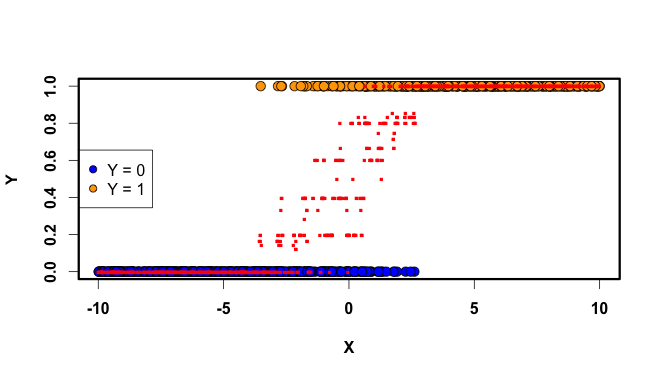
\includegraphics[width=14cm]{../fig/Cap13-ClasificadorKnn01.png}\\[2mm]
\end{enColor}
\begin{bn}
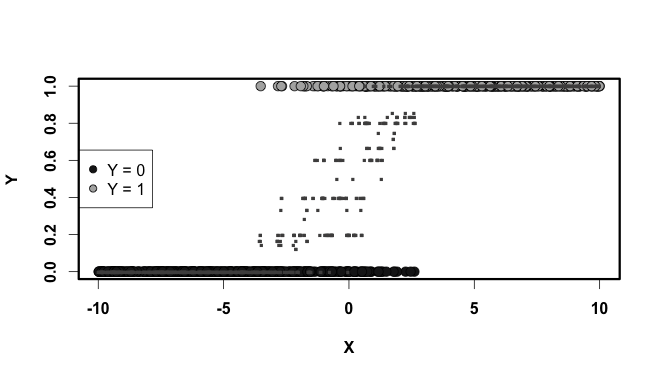
\includegraphics[width=14cm]{../fig/Cap13-ClasificadorKnn01-bn.png}\\[2mm]
\end{bn}
(b)\\[2mm]
\begin{enColor}
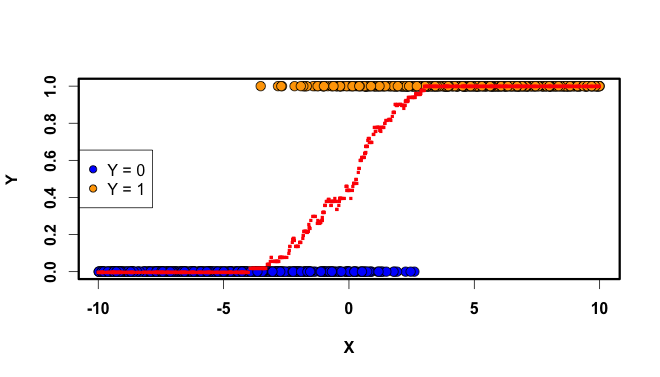
\includegraphics[width=14cm]{../fig/Cap13-ClasificadorKnn02.png}
\end{enColor}
\begin{bn} 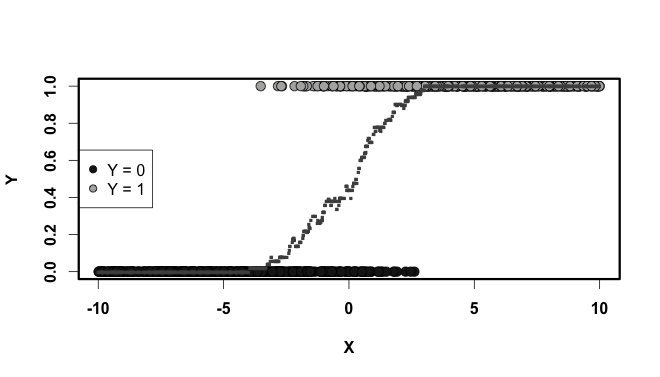
\includegraphics[width=14cm]{../fig/Cap13-ClasificadorKnn02-bn.png}
\end{bn}
\caption{Estimaciones de probabilidad por el método de clasificación
knn en el Ejemplo \ref{cap13:ejem:clasificadorKnn}. En la parte (a) se ha usado $k=5$, mientras que en la parte (b) usamos $k=100$.	}
\label{cap13:fig:ClasificadorKnn}
\end{center}
\end{figure}
\qed	
\end{ejemplo}
	
Una ventaja evidente del método knn es que es fácil de generalizar a otras situaciones. Por ejemplo, para clasificación politómica o en problemas con más de una variable predictora. Pero, a la vista de este ejemplo, está claro que hemos dejado pendiente una pregunta básica que te debes estar haciendo: ¿cómo se selecciona el {\em mejor} valor de $k$ en el método knn y cómo podemos controlar a la vez el valor de $k$ y el umbral $c_p$? Más aún, ¿en qué sentido o sentidos es mejor un valor de $k$ que otro? Relacionado con esto,  el punto más débil de este método es la definición de la forma de medir la distancia que usamos al definir los {\em vecinos cercanos}. En el ejemplo que hemos visto se supone que las diferencias entre valores de $X$ son relevantes en el problema que nos ocupa. Pero en otros problemas, la elección de la distancia adecuada, si es que somos capaces de hallarla, es un asunto realmente complicado y, si el lector quiere aprender más sobre este tema y aplicar estos métodos a problemas con varias variables de distintos tipos, entonces tendrá necesariamente que profundizar en la noción matemática de métrica. En cualquier caso, no vamos a extendernos más aquí sobre este método, que tiene su lugar natural en un curso de introducción al Aprendizaje Automático. El lector interesado encontrará algunas indicaciones y referencias en el Apéndice \ref{apendice:MasAlla}.

\subsubsection{Clasificador aleatorio.}

El método que vamos a describir a continuación juega un papel especial en la teoría a la hora de comparar entre sí distintos métodos de clasificación para decidir cuál es el mejor. Por esa razón tiene algunas peculiaridades que pueden resultar un poco desconcertantes al principio.

En el método de clasificación basado en la regresión logística teníamos que elegir un punto de corte $c_p$. En el método $knn$ elegíamos el valor de $k$. En el clasificador aleatorio también tenemos que elegir un valor, concretamente un valor de $p$ entre $0$ y $1$.  Y entonces, cada vez que tenemos que predecir el  valor $\hat{Y}(x)$ respondemos $1$ o $0$ con probabilidad $p$ para el valor $1$ y probabilidad $q =1 - p$ para el valor $0$. Antes hemos hablado de predecir los valores lanzando una moneda. El clasificador aleatorio hace precisamente eso, con la salvedad de que la moneda está cargada con probabilidad $p$.

Como ves, un ``clasificador'' aleatorio no hace ningún esfuerzo por ``clasificar'' y se limita a asignar sus predicciones al azar.  Y eso se traduce en una diferencia básica con los ejemplos que hemos visto antes: incluso con una muestra fija las predicciones $\hat{Y}(x)$ que se obtienen con el clasificador aleatorio para un mismo valor de $X$ pueden ser distintas cada vez que se usa este ``clasificador''. Eso no sucedía con el clasificador knn ni con el clasificador por umbral basado en regresión logística.


Y entonces ¿para que nos sirve este presunto clasificador aleatorio? Cuando, en este y en capítulos anteriores, hemos comparado modelos estadísticos, nos ha resultado útil pensar en términos de señal y ruido. Para que un modelo estadístico tenga algún valor, tiene que aportar algo frente al ``modelo'' en que todo es ruido y no hay señal. Aquí no estamos comparando modelos estadísticos, sino clasificadores. Pero la idea sigue sirviéndonos: el clasificador aleatorio juega ese mismo papel de todo ruido y nada de señal. {\em Para que un clasificador se merezca el nombre, tiene que hacer su trabajo mejor que el clasificador aleatorio.} ¿Cómo podemos comprobar eso? Es decir, ¿cómo medimos la calidad de un clasificador? En las próximas secciones nos vamos a ocupar de este problema. Para empezar, vamos a descubrir que en realidad ya hemos desarrollado mucho vocabulario para este tipo de problemas.

\subsubsection*{Y hay muchas otras  estrategias.}

Aparte de los que hemos visto, hay una gran diversidad de métodos clasificadores. Por citar algunos: clasificadores bayesianos, análisis discriminante, árboles de decisión, redes neuronales, máquinas de soporte vectorial, etc. Muchas de esas ideas van más allá del ámbito tradicional de la Estadística, para situarse en el terreno de lo que se ha dado en llamar {\em Análisis de Datos}. En el Apéndice \ref{apendice:MasAlla} daremos algunas indicaciones adicionales.


\subsection{Clasificadores dicotómicos y pruebas diagnósticas.}
\label{cap13:subsec:ClasificadoresDicotomicosPruebasDiagnosticas}

La pregunta que queremos hacernos en esta sección es fácil de formular: dado un método de clasificación ¿cómo podemos medir la calidad de sus resultados? Dicho de otra manera ¿cómo de fiable es la clasificación que proporciona el método? En principio, vamos a seguir centrando nuestra atención en el mismo tipo especial de problemas de clasificación: una variable respuesta $Y$ dicotómica (factor con dos niveles) con una variable predictora $X$ cuantitativa. Dentro de estos, en los ejemplos prestaremos especial atención  a los métodos de clasificación  que usan la regresión logística con un valor umbral $c_p$ como modelo de clasificación.

Decíamos al final del apartado anterior, y lo vamos a comprobar enseguida, que ya hemos desarrollado una gran cantidad de lenguaje para los problemas de clasificación. Concretamente, vamos a ver que existe una relación entre estos problemas y las pruebas diagnósticas que ya han aparecido varias veces en el libro. En efecto, si la variable respuesta es dicotómica, con valores $0$ y $1$, entonces cuando usamos un algoritmo de clasificación obtendremos resultados que también vendrán en forma de unos y ceros. Para evaluar la calidad de esos resultados vamos a suponer que disponemos de una muestra en la que aparecen los valores observados (y por tanto correctamente clasificados) de la variable de interés $Y$. Si vamos a medir la calidad de la clasificación que proporciona el método es esencial disponer de esos valores correctos de $Y$ para poder compararlos con las predicciones que produce el método al aplicarlo a esa muestra.  Podemos entonces formar una tabla de contingencia de doble entrada en la que indicaremos los resultados del método frente a los valores correctos, como la Tabla \ref{cap13:tabla:TablaContingenciaClasificadorDicotomico}.

\begin{table}[ht]
	\begin{center}
		\begin{tabular}{cc|c|c|c|}
			&\multicolumn{1}{c}{}&\multicolumn{3}{c}{\bf Valor correcto:}\\
			\cline{3-5}
			% after \\: \hline or \cline{col1-col2} \cline{col3-col4} ...
			&\multicolumn{1}{c|}{}& $Y = 1$&  $Y = 0$& Total \\
			\cline{2-5}
			{\bf Resultado del método:}&\multicolumn{1}{|c|}{\rule{0cm}{0.5cm}$\hat{Y} = 1$}& $n_{11}$ & $n_{12}$ & $n_{1+}$ \\ % 11 8 19
			\cline{2-5}
			& \multicolumn{1}{|c|}{\rule{0cm}{0.5cm}$\hat{Y} = 0$ }& $n_{21}$ & $n_{22}$ &  $n_{2+}$\\ % 4  7 11
			\cline{2-5}
			& \multicolumn{1}{|c|}{Total} & $n_{+1}$ & $n_{+2}$ & $n$ \\
			\cline{2-5}
		\end{tabular}
	\end{center}
	\caption{Tablas de contingencia para un método de clasificación dicotómica.}
	\label{cap13:tabla:TablaContingenciaClasificadorDicotomico}
\end{table}

Al ver esa tabla el lector sin duda habrá pensado en la Tabla \ref{cap03:tabla:notacionTablaContingencia} (pag. \pageref{cap03:tabla:notacionTablaContingencia})  de las pruebas diagnósticas. Una prueba diagnóstica como las que describimos entonces es un ejemplo de problema de clasificación. Pero para lo que nos interesa aquí lo más importante es que podemos ver las cosas al revés: cualquier método clasificador dicotómico se puede ver como una prueba diagnóstica. Así que al analizar estos métodos podemos reutilizar todo el lenguaje que desarrollamos para las pruebas diagnósticas, algo que ya apuntamos en el Ejemplo \ref{cap13:ejem:ClasificadorIngenuo} (pág. \pageref{cap13:ejem:ClasificadorIngenuo}). Hagamos un breve repaso de la terminología básica, adaptándola al problema de clasificación antes de ver un ejemplo:

\begin{itemize}

	\item Los {\em falsos positivos} y los {\em falsos negativos} aparecen reflejados en los elementos $n_{12}$ y $n_{21}$ de la tabla, los que están situados fuera de la diagonal principal. En el lenguaje de los problemas de clasificación, estos dos tipos de situaciones corresponden a los errores de clasificación del método.

	\item Por contra, los elementos de la diagonal principal $n_{11}$ y $n_{22}$ muestran los casos en los que el método ha acertado al producir una clasificación correcta. Hay dos cantidades directamente relacionadas con esos valores. La {\em sensibilidad} es
	\[\mbox{sensibilidad}=P(\mbox{clasificado como 1}\,|\,\mbox{valor correcto = 1})=\dfrac{n_{11}}{n_{+1}}.\]
	Por su parte la {\em especificidad} es
	\[\mbox{especificidad}=P(\mbox{clasificado como 0}\,|\,\mbox{valor correcto = 0})=
	\dfrac{n_{22}}{n_{+2}}.\]
	
	\item Las dos anteriores nociones nos eran conocidas desde el  Capítulo  \ref{cap:Probabilidad}. Para obtener una primera medida conjunta de la calidad del método de clasificación se puede usar (entre otras)  la {\sf tasa de acierto}\index{tasa de acierto de un método clasificador} (en inglés, {\em accuracy})\index{accuracy for classifiers}, que se define así:
	\[\mbox{tasa de acierto} = \dfrac{n_{11} + n_{22}}{n}.\]
\end{itemize}
Vamos a ver cómo calcular estas cantidades en un ejemplo concreto de  clasificación mediante regresión logística usando un valor umbral $c_p$.

\begin{Ejemplo}
\label{cap13:ejem:ROC0}
	
La parte (a) de la Tabla \ref{cap13:tabla:ejemploClasificadorVasculopatia1} (pág. \pageref{cap13:tabla:ejemploClasificadorVasculopatia1}) contiene  los datos del Ejemplo \ref{cap13:ejem:RegresionLogistica00}(pág.  \pageref{cap13:ejem:RegresionLogistica00}) sobre la relación entre el itb y la vasculopatía. La tercera columna contiene los valores observados correctos de la variable respuesta $Y$. Esta columna recoge la información clave para  evaluar la calidad de un método de clasificación. La segunda columna (titulada $\hat{\pi}$) contiene las estimaciones  de la probabilidad $ P(Y=1|X=x)$ obtenidas con un modelo de  regresión logística ajustado a estos datos.  Además, hemos tomado como umbral el valor $c_p=0.5$, el correspondiente al método de clasificación que hemos llamado ingenuo en la página \pageref{cap13:subsubsec:MetodoIngenuoClasificacion}. Usando ese método hemos obtenido las clasificaciones de las  observaciones, que aparecen en la cuarta columna de la tabla. Comparando esas clasificaciones con los valores correctos (los valores $Y$) se obtiene la tabla de contingencia que aparece en la parte (b) de la Tabla \ref{cap13:tabla:ejemploClasificadorVasculopatia1}.

Esa tabla nos muestra que hay dos valores mal clasificados del total de $30$. Y a partir de esa tabla se obtiene:

\[
\begin{cases}
\mbox{sensibilidad} = \dfrac{10}{11}\approx 0.9091\\[5mm]
\mbox{especificidad} = \dfrac{18}{19}\approx 0.9474\\[5mm]
\mbox{tasa de acierto} = \dfrac{10 + 18}{30}\approx 0.9333
\end{cases}
\]

\begin{table}[btp]
\begin{center}
{\small	
	(a)\\[3mm]
\begin{tabular}{rcccc}
	\hline
\rule{0cm}{0.5cm}& X (itb) & $\hat{\pi}$ & Y (vasculopatía)& $\hat{Y}$ (clasificación) \\
	\hline
1 & 1.42 & 0.00 & 0 & 0 \\
2 & 1.35 & 0.00 & 0 & 0 \\
3 & 1.29 & 0.00 & 0 & 0 \\
4 & 1.25 & 0.00 & 0 & 0 \\
5 & 1.25 & 0.00 & 0 & 0 \\
6 & 1.22 & 0.00 & 0 & 0 \\
7 & 1.12 & 0.00 & 0 & 0 \\
8 & 1.12 & 0.00 & 0 & 0 \\
9 & 1.10 & 0.00 & 0 & 0 \\
10 & 1.04 & 0.01 & 0 & 0 \\
11 & 1.02 & 0.02 & 0 & 0 \\
12 & 1.00 & 0.04 & 0 & 0 \\
13 & 0.99 & 0.06 & 0 & 0 \\
14 & 0.98 & 0.08 & 0 & 0 \\
15 & 0.98 & 0.08 & 0 & 0 \\
16 & 0.95 & 0.18 & 1 & 0 \\
17 & 0.94 & 0.24 & 0 & 0 \\
18 & 0.93 & 0.30 & 0 & 0 \\
19 & 0.92 & 0.38 & 0 & 0 \\
20 & 0.90 & 0.54 & 1 & 1 \\
21 & 0.88 & 0.69 & 1 & 1 \\
22 & 0.88 & 0.69 & 1 & 1 \\
23 & 0.86 & 0.82 & 0 & 1 \\
24 & 0.84 & 0.90 & 1 & 1 \\
25 & 0.79 & 0.98 & 1 & 1 \\
26 & 0.70 & 1.00 & 1 & 1 \\
27 & 0.64 & 1.00 & 1 & 1 \\
28 & 0.62 & 1.00 & 1 & 1 \\
29 & 0.50 & 1.00 & 1 & 1 \\
30 & 0.44 & 1.00 & 1 & 1 \\
	\hline
\end{tabular}\\[5mm]
(b)\\[3mm]

\begin{tabular}{lcccc}
         	$c_p=0.5$ &&\multicolumn{2}{c}{\bf Vasculopat\'ia} $Y$&\\
         	&&\multicolumn{2}{c}{\underline{\vspace{.25cm}(observado)}}&\\
         	
         	&          & Sí &  No & Total\\
         	\hline
         	{\bf Diagnóstico} & + & 10 &  1 & 11\\
         	(predicción modelo ingenuo) & $-$ & 1 & 18 & 19\\
         	\hline
         	& Total    & 11& 19 & 30\\
         	\hline
\end{tabular}
}		
\end{center}
		\caption{Tablas del Ejemplo \ref{cap13:ejem:ROC0}, pag. \pageref{cap13:ejem:ROC0}.}
		\label{cap13:tabla:ejemploClasificadorVasculopatia1}
\end{table}

\qed
\end{Ejemplo}
Antes de entrar a juzgar resultados como los de este ejemplo,  conviene tener claro cuál es la escala en la que los medimos. En concreto, ¿cuál sería el caso ideal? A primera vista parece natural elegir aquel en el que el método de clasificación tiene una tasa de acierto igual a 1. Es decir, que no hay errores de clasificación.  Eso significa que en el caso del clasificador ideal la Tabla de contingencia \ref{cap13:tabla:TablaContingenciaClasificadorDicotomico}  (pág. \pageref{cap13:tabla:TablaContingenciaClasificadorDicotomico} ) tiene $n_{12} = n_{21} = 0$. En otras palabras, los elementos  situados fuera de la diagonal principal son cero.  Por lo tanto, nuestra primera impresión es que para un clasificador ideal se tendría
\[
\begin{cases}
\mbox{sensibilidad} = 1\\[4mm]
\mbox{especificidad} = 1\\[4mm]
\mbox{tasa de acierto} = 1
\end{cases}
\]
Pero, como sucede a menudo, las cosas van a resultar más complicadas y, por tanto, más divertidas. En este punto queremos recordar que hemos dejado pendiente el problema de comparar clasificadores. Y, como caso especial de ese problema, también hemos dejado pendiente la forma de elegir el valor umbral o punto de corte $c_p$ que se utiliza en el clasificador logístico o el valor de $k$ que usamos en el clasificador knn. ¿Podemos usar medidas como la sensibilidad, especificidad o la tasa de acierto para ayudarnos a decidir? Ese es el tema del próximo apartado.

\subsection{Comparación de clasificadores. }
\label{cap13:subsection:seleccionPuntoCorte}

¿Qué ocurre con el clasificador logístico al cambiar el valor del punto de corte $c_p$? Recuerda la definición del clasificador por umbral que dimos en la Ecuación \ref{cap13:ecu:clasificadorLogisticoUmbral} (pág. \pageref{cap13:ecu:clasificadorLogisticoUmbral}):

\begin{equation*}
\hat Y(x) =
\begin{cases}
	0 &\mbox{si } \hat{\pi}(x) < c_p,\\[3mm]
	1 &\mbox{si } \hat{\pi}(x) \geq c_p.
\end{cases}	
	\tag{\ref{cap13:ecu:clasificadorLogisticoUmbral} repetida.}
\end{equation*}

Puesto que las probabilidades $\hat{\pi}(x)$ son valores comprendidos entre $0$ y $1$ sólo tiene sentido hacer que $c_p$ varíe entre esos mismos dos valores. ¿Qué sucede en los casos extremos?

\begin{itemize}
	\item Cuando tomamos $c_p=0$ estamos haciendo $\hat Y(x) =1$ para todas las observaciones. En la notación de la tabla de contingencia \ref{cap13:tabla:TablaContingenciaClasificadorDicotomico} (pág. \pageref{cap13:tabla:TablaContingenciaClasificadorDicotomico}) eso significa
	\[n_{11}= n_{+1},\quad n_{12}= n_{+2},\quad n_{21}= 0,\quad n_{22}= 0.\]
	En consecuencia, dado que  todas las observaciones se clasifican como positivos,  la sensibilidad es $1$.  La especificidad, en cambio, es $0$.
	
	\item Por contra, cuando tomamos $c_p=1$ estamos haciendo $\hat Y(x) =0$ para todas las observaciones.  Excepto, desde luego, para aquellas que tuvieran $\hat\pi(x)=1 $. En el modelo de regresión logística, esos valores $1$ no se dan, salvo por el redondeo.  Si se usan otros modelos clasificadores las cosas pueden ser distintas, desde luego. Pero suponiendo que $\hat Y(x) =0$ para todas las observaciones, eso significa que:
	\[n_{11}= 0,\quad n_{12}= 0,\quad n_{21}= n_{+1},\quad n_{22}= n_{+2}.\]
	Y entonces, dado que  todas las observaciones se clasifican como negativos,  la sensibilidad es $0$, mientras que la especificidad, en cambio, es $1$.
	
\end{itemize}
En resumen: a medida que $c_p$ aumenta desde $0$ hasta $1$, la sensibilidad disminuye desde $1$ hasta $0$, mientras que la especificidad aumenta desde $0$ hasta $1$.

\begin{ejemplo}
\label{cap13:ejem:CurvasSensibilidadEspecificidad}
Vamos a usar de nuevo los datos del modelo que relaciona el índice itb con la vasculopatía. Si representamos la forma en la que cambian los valores de la sensibilidad y especificidad del clasificador logístico a medida que $c_p$ recorre el intervalo $[0, 1]$ obtenemos para esos datos las dos curvas que aparecen en la Figura \ref{cap13:fig:CurvasSensibilidadEspecificidad}.
Las curvas son poligonales porque nuestra muestra tiene una cantidad finita de puntos. Por lo tanto, nuestro modelo sólo tiene una cantidad finita de valores de las probabilidades $\hat{\pi}(x)$. Eso, a su vez, se traduce en que aunque modifiquemos el valor de $c_p$, la tabla de contingencia del clasificador sólo puede cambiar, a saltos, cuando $c_p$ va pasando por cada uno de los valores $\hat{\pi}(x)$. Esos cambios de la tabla de contingencia son los que pueden traducirse en cambios de la sensibilidad y especificidad.   En cualquier caso, a la vista de la figura  está claro que en este ejemplo es imposible elegir un valor del punto de corte para el que tanto la sensibilidad como la especificidad valgan ambas $1$.  Tenemos que llegar a un compromiso. ¿Cómo?

\begin{figure}[h!]
\begin{center}
\begin{enColor}
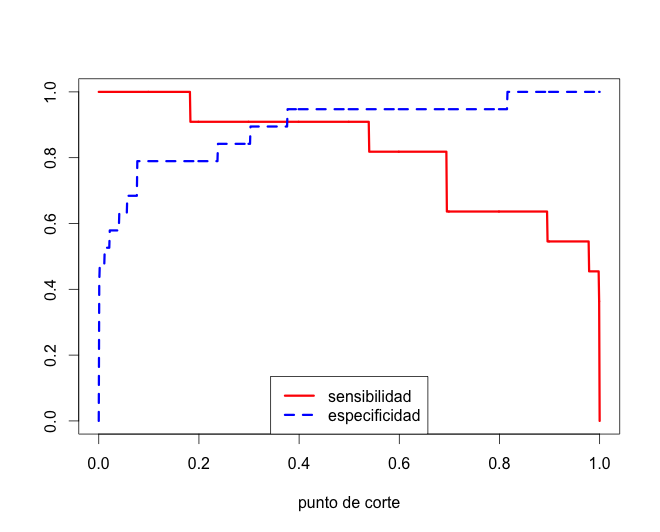
\includegraphics[width=13cm]{../fig/Cap13-CurvasSensibilidadEspecificidad.png}
\end{enColor}
\begin{bn}
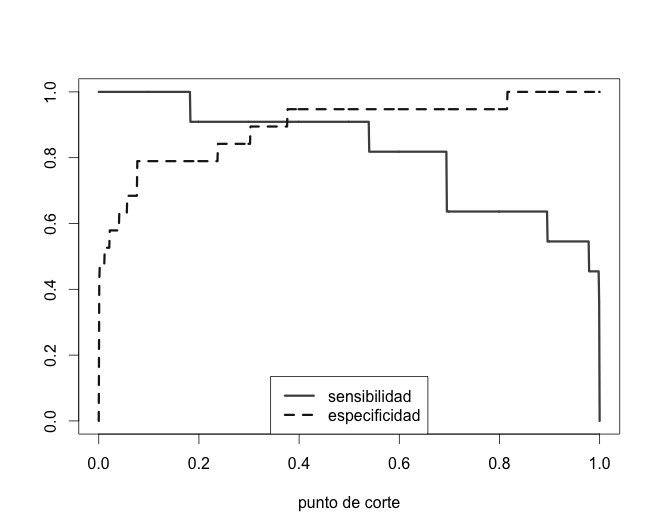
\includegraphics[width=13cm]{../fig/Cap13-CurvasSensibilidadEspecificidad-bn.png}
\end{bn}
\caption{Sensibilidad y especificidad en función del punto de corte
$c_p$ en el Ejemplo \ref{cap13:ejem:CurvasSensibilidadEspecificidad}. }
\label{cap13:fig:CurvasSensibilidadEspecificidad}
\end{center}
\end{figure}

\qed
\end{ejemplo}

La situación que hemos encontrado en el Ejemplo \ref{cap13:ejem:CurvasSensibilidadEspecificidad} es muy representativa de lo que suele ocurrir en este tipo de problemas.  Puesto que en este problema hay dos características deseables (la sensibilidad y la especificidad) a menudo sucederá que no podemos hacer máximas ambas a la vez. En muchos casos, existe alguna razón que nos lleva a privilegiar la sensibilidad frente a la especificidad o viceversa. Pero si no es así y tratamos de buscar un equilibrio entre ambas características nos tendremos que conformar con algún tipo de compromiso. Una manera típica de hacerlo es buscando una cantidad que sea algún tipo de  combinación, o mezcla si prefieres pensarlo así, de la sensibilidad y la especificidad  y entonces buscar el valor de $c_p$ que hace máxima esa combinación. Si la combinación se ha definido de manera sensata, eso nos puede proporcionar el tipo de respuesta que andamos buscando.  ¿Podríamos usar la tasa de aciertos? Vamos a empezar explorando este enfoque, ilustrándolo de nuevo con un ejemplo.

\begin{ejemplo}
\label{cap13:ejem:CurvaTasaAciertos}
Si con los datos de itb y vasculopatía representamos la tasa de aciertos para distintos valores  del punto de corte obtenemos
la Figura \ref{cap13:fig:TasaAciertosVsPuntoCorte}. Esa figura muestra que hay todo un intervalo de valores posibles de $c_p$, cercanos a $0.5$, que hacen máximo el valor de la tasa de aciertos. Podemos tomar entonces como valor el punto medio de ese intervalo, que en este ejemplo es aproximadamente $c_p = 0.45$.

	\begin{figure}[h!]
		\begin{center}
			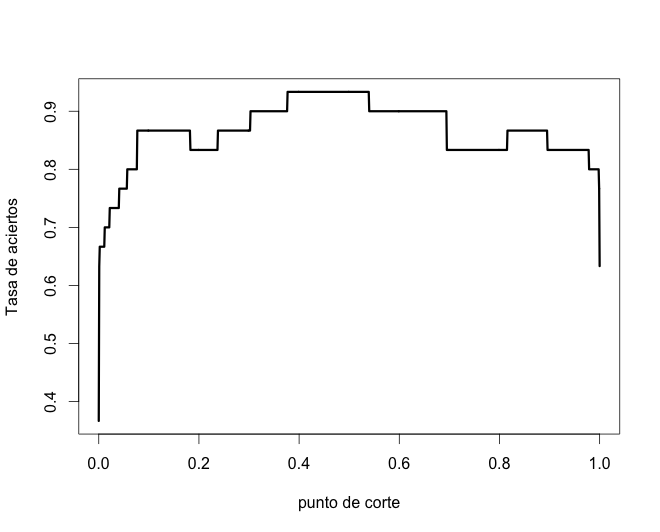
\includegraphics[width=13cm]{../fig/Cap13-TasaAciertosVsPuntoCorte.png}
			\caption{Tasa de aciertos en función del punto de corte $c_p$ en el Ejemplo \ref{cap13:ejem:CurvaTasaAciertos}. }
			\label{cap13:fig:TasaAciertosVsPuntoCorte}
		\end{center}
	\end{figure}

\qed		
\end{ejemplo}
Aunque este enfoque basado en la tasa de aciertos se usa a menudo para hacerse una idea de la calidad de una clasificación dicotómica, hay que tener bastante precaución y no olvidarse de examinar la tabla de contingencia. El siguiente ejemplo trata de aclarar el por qué de esta advertencia.
\begin{ejemplo}
	\label{cap13:ejem:ProblemasTasaAciertos}
Imagínate un clasificador dicotómico cuya tabla de contingencia es la parte (a) de la Tabla \ref{cap13:tabla:ProblemasTasaAciertos}.  Con esos valores, la tasa de aciertos del clasificador es del $94\%$. Puede parecer bastante buena, pero se debe exclusivamente a una sensibilidad muy alta (90 de 92 aciertos), mientras que la especificidad es muy baja (4 de 8 aciertos). Y si miras la parte (b) de la tabla, comprenderás que las cosas son aún peores: con la misma tasa de aciertos ahora los papeles se han cambiado: es la especificidad la que es muy alta ($93$ aciertos de $94$) mientras que la sensibilidad es una calamidad ($1$ acierto de $6$).

\begin{table}[ht]
	\begin{center}
		(a)\quad
		\begin{tabular}{cc|c|c|c|}
			&\multicolumn{1}{c}{}&\multicolumn{3}{c}{\bf Valor correcto:}\\
			\cline{3-5}
			% after \\: \hline or \cline{col1-col2} \cline{col3-col4} ...
			&\multicolumn{1}{c|}{}& $Y = 1$&  $Y = 0$& Total \\
			\cline{2-5}
			{\bf Clasificación}&\multicolumn{1}{|c|}{\rule{0cm}{0.5cm}$\hat{Y} = 1$}& $90$ & $4$ & $94$ \\
			\cline{2-5}
			& \multicolumn{1}{|c|}{\rule{0cm}{0.5cm}$\hat{Y} = 0$ }& $2$ & $4$ &  $6$\\
			\cline{2-5}
			& \multicolumn{1}{|c|}{Total} & $92$ & $8$ & $100$ \\
			\cline{2-5}
		\end{tabular}
		\\[5mm]
		(b)\quad
		\begin{tabular}{cc|c|c|c|}
			&\multicolumn{1}{c}{}&\multicolumn{3}{c}{\bf Valor correcto:}\\
			\cline{3-5}
			% after \\: \hline or \cline{col1-col2} \cline{col3-col4} ...
			&\multicolumn{1}{c|}{}& $Y = 1$&  $Y = 0$& Total \\
			\cline{2-5}
			{\bf Clasificación}&\multicolumn{1}{|c|}{\rule{0cm}{0.5cm}$\hat{Y} = 1$}& $1$ & $1$ & $2$ \\
			\cline{2-5}
			& \multicolumn{1}{|c|}{\rule{0cm}{0.5cm}$\hat{Y} = 0$ }& $5$ & $93$ &  $98$\\
			\cline{2-5}
			& \multicolumn{1}{|c|}{Total} & $6$ & $94$ & $100$ \\
			\cline{2-5}
		\end{tabular}		
	\end{center}
	\caption{Tablas de contingencia del Ejemplo \ref{cap13:ejem:ProblemasTasaAciertos}.}
	\label{cap13:tabla:ProblemasTasaAciertos}
\end{table}

\qed		
\end{ejemplo}
 La conclusión del ejemplo precedente refuerza el mensaje que hemos recibido varias veces a lo largo del curso: tratar de reducir el análisis de la calidad de un modelo o método a un único número a menudo es una simplificación sin justificación. El usuario de la Estadística tiene que estar siempre atento a toda una colección de herramientas de análisis para poder juzgar con propiedad la validez de los resultados.   Otra manera de ver el problema que hemos detectado en el Ejemplo \ref{cap13:ejem:ProblemasTasaAciertos} consiste en estudiar con más detalle la relación entre la tasa de aciertos y la sensibilidad y especificidad. Tenemos:

 \[
 \mbox{tasa de aciertos} = \dfrac{n_{11} + n_{22}}{n} = \dfrac{n_{11}}{n} + \dfrac{n_{22}}{n}  =
\left(\dfrac{n_{11}}{n_{+1}}\right) \cdot \left(\dfrac{n_{+1}}{n}\right) +
\left(\dfrac{n_{22}}{n_{+2}}\right) \cdot  \left(\dfrac{n_{+2}}{n}\right) =
 \]
 \[
\left( \mbox{sensibilidad}\right)\cdot k +  \left(\mbox{especificidad}\right)\cdot (1 - k)
 \]
 donde es fácil reconocer que
 \[
 k = \dfrac{n_{+1}}{n}
 \]
 es la cantidad que, en el contexto de las pruebas diagnósticas, llamábamos {\em prevalencia} (la proporción de enfermos en la población). Así que el problema es que la tasa de errores hace intervenir a la sensibilidad y especificidad, pero en la mezcla se nos ha colado un invitado inesperado, la prevalencia, que interfiere en el análisis.

 \begin{ejemplo}{\bf (Continuación del Ejemplo \ref{cap13:ejem:ProblemasTasaAciertos})}
 	\label{cap13:ejem:ProblemasTasaAciertos2}
 En la 	parte (a) de la Tabla \ref{cap13:tabla:ProblemasTasaAciertos} la prevalencia es del $92\%$, mientras que en la parte (b) es del $6\%$. Esa diferencia tan pronunciada en el valor de la prevalencia explica las diferencias que hemos discutido en el Ejemplo \ref{cap13:ejem:ProblemasTasaAciertos}, pero que la tasa de errores no es capaz de detectar por sí misma.
 	
 \qed	
\end{ejemplo}


La conclusión de estos ejemplos es que la tasa de errores depende mucho de un factor ajeno a la calidad intrínseca de nuestro método clasificado, porque esa tasa se ve fuertemente condicionada por la distribución de las dos clases en la población.


\subsection{Curvas ROC y área bajo la curva ROC.}
\label{cap13:subsection:ROC}

% How well can this classifier be expected to perform in general, at a variety of different baseline probabilities?", go with a ROC curve.

% http://stats.stackexchange.com/questions/16998/accuracy-of-a-random-classifier

Las últimas reflexiones de la sección anterior nos hacen pensar en que sería bueno tener una medida de la calidad de un clasificador por umbral que sólo dependiera de los valores de la sensibilidad y la especificidad. Lo que hace interesante a estas dos cantidades es que miden la tasa de aciertos de la prueba {\em dentro de cada nivel del factor}. Y eso las hace resistentes a cambios en la composición de la población. El problema es que, como hemos visto, no es posible hacer máximas las dos a la vez.  Si, con esas idea en mente,  repasas la Sección \ref{cap03:sec:OddsPruebasDiagnosticas} (pág. \pageref{cap03:sec:OddsPruebasDiagnosticas}) encontrarás la Ecuación \ref{cap03:ecu:RelacionBayesianaOddsPrePostTestPositivo} (pág. \pageref{cap03:ecu:RelacionBayesianaOddsPrePostTestPositivo}), que reproducimos aquí por comodidad:
\begin{equation}\tag{\ref{cap03:ecu:RelacionBayesianaOddsPrePostTestPositivo} repetida.}
\left(\mbox{Odds $D$ post-prueba positiva}\right)=RVP\cdot \left(\mbox{Odds $D$ pre-prueba}\right).
\end{equation}
donde $RVP$ es la {\em razón de verosimilitud positiva}, definida mediante (ver pág. \pageref{cap03:ecu:RazonVerosimilitudPositiva} )
\[
RVP=\dfrac{\mbox{sensibilidad}}{\alpha}=\dfrac{\mbox{sensibilidad}}{1-\mbox{especificidad}}
\]
Al discutir las pruebas diagnósticas dijimos que la Ecuación \ref{cap03:ecu:RelacionBayesianaOddsPrePostTestPositivo} permite, de una manera muy sencilla, actualizar nuestro cálculo de las posibilidades (odds) de un diagnóstico de enfermedad, una vez obtenido un resultado positivo en la prueba. Y el ingrediente clave de esa ecuación es el factor $RVP$, la razón de verosimilitud positiva, que a su vez depende de la sensibilidad y la especificidad de la prueba. Vamos a pensarlo con un poco de cuidado:
\begin{itemize}
  \item A la luz de la Ecuación \ref{cap03:ecu:RelacionBayesianaOddsPrePostTestPositivo}, si $RVP = 1$ entonces el resultado positivo de la prueba diagnóstica no ha cambiado nada nuestra estimación de las posibilidades.  Dicho de forma más sencilla: la prueba no nos ha ayudado nada a clasificar al paciente como enfermo.

  \item En cambio, un valor muy grande de $RVP$ significa que si la prueba diagnóstica es positiva, entonces las posibilidades a favor de que el paciente esté realmente enfermo aumentan mucho.
\end{itemize}

Naturalmente, hay un problema con el denominador de $RVP$ cuando la especificidad es igual a $1$. Pero, de nuevo, si lo piensas, una prueba diagnóstica con especificidad igual a $1$ es una prueba sin falsos positivos. Es decir, que en ese caso la clasificación que proporciona un resultado positivo es incuestionable.

Volviendo sobre el caso $RVP=1$, es fácil ver que eso significa que en la tabla de contingencia se cumple:
\[
\left(\dfrac{n_{11}}{n_{+1}}\right) = \left(\dfrac{n_{12}}{n_{+2}}\right)
\]
Y traduciéndolo a palabras: la proporción de positivos que produce nuestra prueba diagnóstica es la misma para los enfermos que para los sanos. Si llamamos $p$ a esa proporción  entonces, esencialmente, nuestra prueba tiene el mismo valor diagnóstico que lanzar una moneda cargada con probabilidad $p$ de acierto. ¿Recuerdas dónde hemos visto esto? En el que llamábamos el {\em clasificador aleatorio}.  Esta es una observación interesante: si sabemos que para un clasificador se cumple
\[
\mbox{sensibilidad} = 1-\mbox{especificidad}
\]
entonces, a todos los efectos,  el clasificador funciona aleatoriamente.

Por razones como estas, a la hora de comparar clasificadores la gente empezó a pensar en estudiar los puntos cuyas coordenadas son esos valores que caracterizan el rendimiento de un clasificador:
\[
(1-\mbox{especificidad}, \mbox{sensibilidad} )
\]
Puesto que la sensibilidad y la especificidad son siempre números entre $0$ y $1$, estos puntos están siempre dentro del cuadrado de lado uno cuyos vértices son los cuatro puntos $(0, 0), (0, 1), (1, 1), (1, 0)$ y que se ilustra en la Figura \ref{cap13:fig:RegionCurvasROC}. Hemos dibujado varios puntos en esa figura para representar distintos algoritmos clasificadores que podemos estar comparando.  La diagonal que conecta los puntos $(0,0)$ y $(1, 1)$ contiene todos los puntos de la forma $(k, k)$ que, como hemos visto,  caracterizan a los clasificadores aleatorios, como el clasificador $A$.
Un buen clasificador debe alejarse de esa diagonal lo más posible, en la dirección del punto $(0, 1)$, que tiene sensibilidad y especificidad ambas iguales a $1$.  Por eso, a la vista de la figura podemos decir que $B$ es un clasificador claramente mejor que $C$. De hecho, $B$ es el mejor clasificador de los que aparecen en esa figura. Pero si  tuviéramos que elegir entre $D$ y $E$ las cosas se complican y necesitaríamos decidir si nos importa más la sensibilidad (elegimos $E$) o la especificidad (elegimos $D$).  ¿Y el clasificador $F$? Ese clasificador, como todos los situados por debajo de la diagonal es {\em ``peor que aleatorio''}. Pero cuidado, podemos estar ante un clasificador realmente bueno. Cuando sucede esto, quiere decir que nuestro clasificador tiene invertidas las clasificaciones, y podemos {\em arreglarlo} simplemente intercambiando sus unos por ceros y viceversa. Es como esa gente a la que pedimos consejo, para luego hacer justo lo contrario de lo que nos recomienden...

\begin{figure}[htb]
\begin{center}
\begin{enColor}
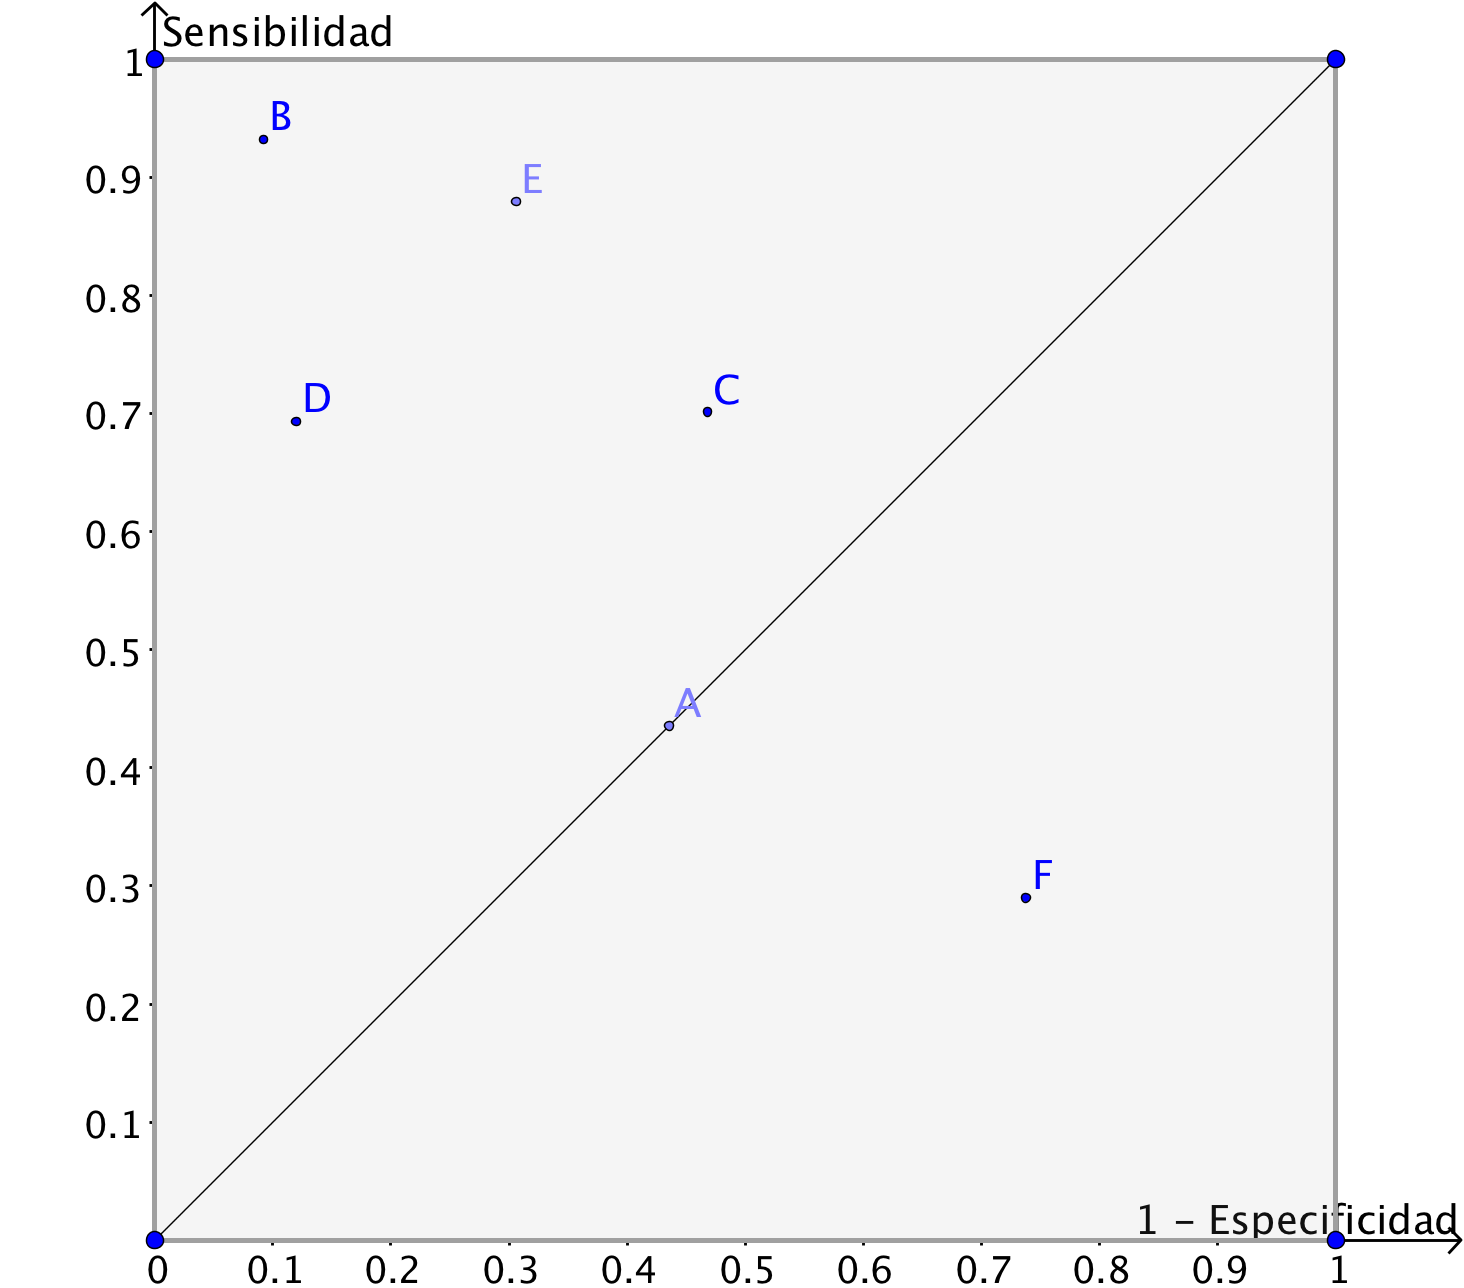
\includegraphics[width=10cm]{../fig/Cap13-RegionCurvasROC.png}
\end{enColor}
\begin{bn}
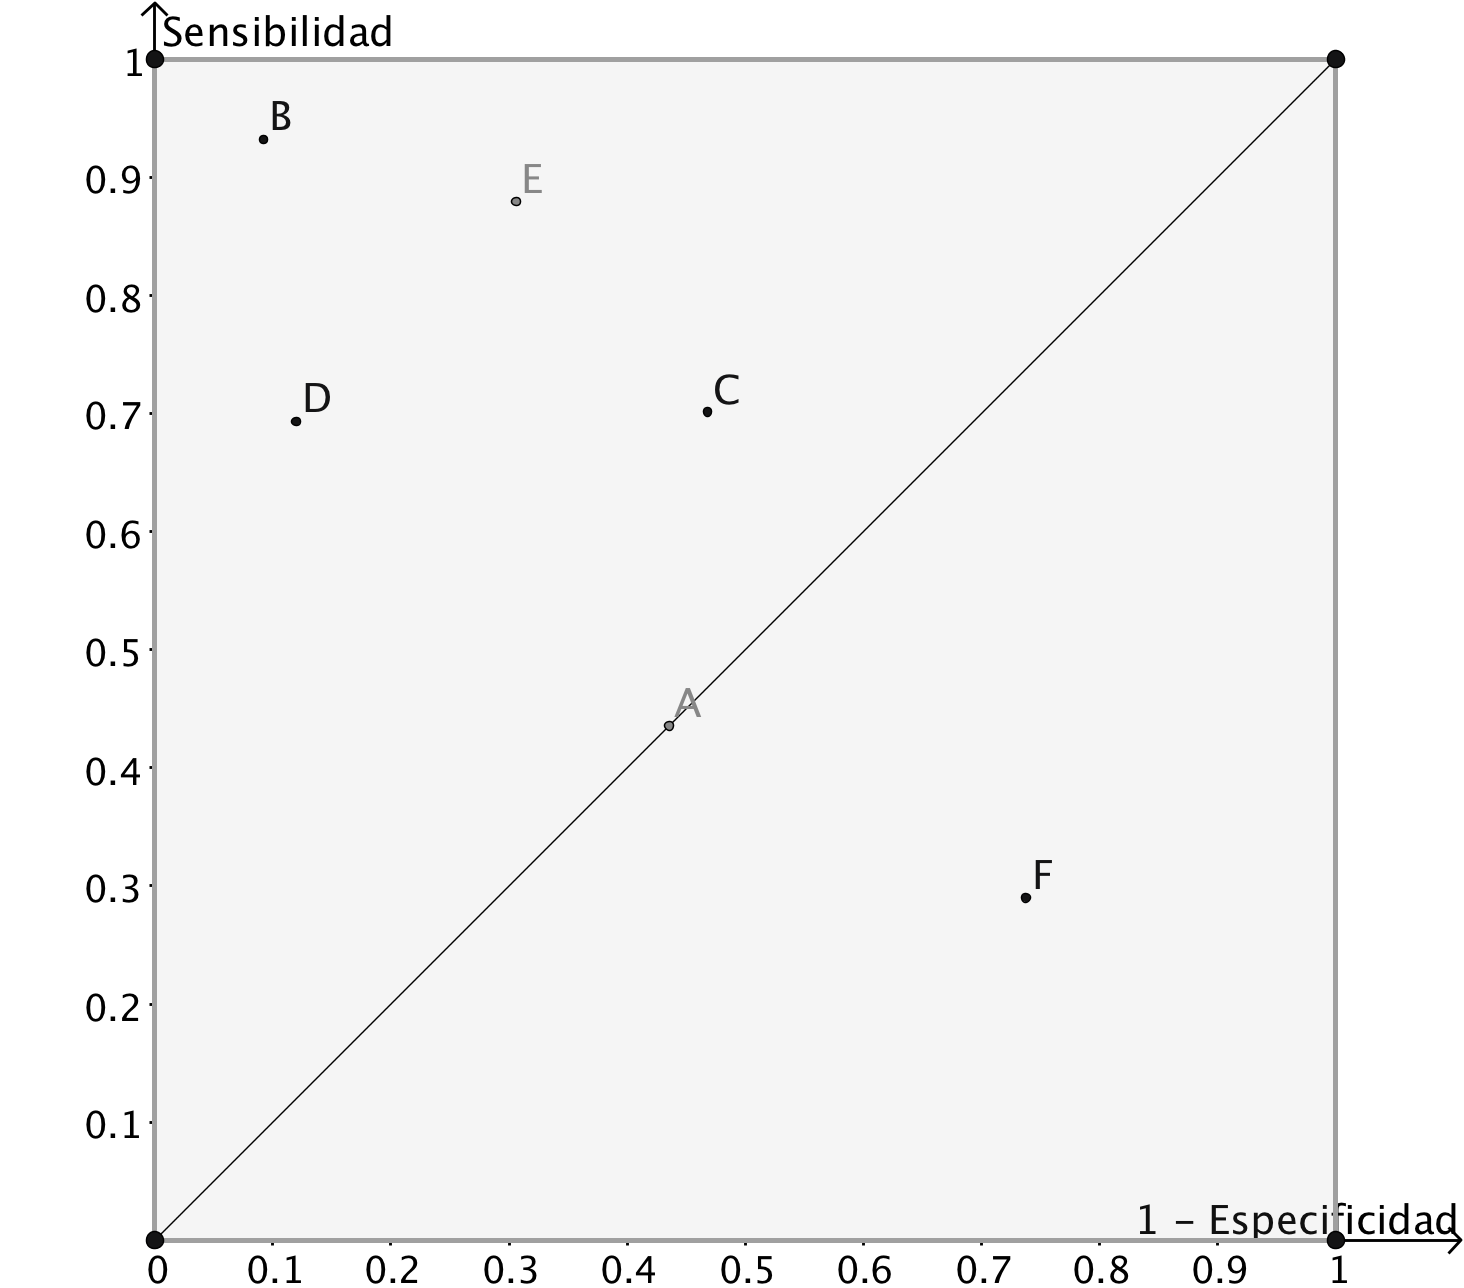
\includegraphics[width=10cm]{../fig/Cap13-RegionCurvasROC-bn.png}
\end{bn}
\caption{El espacio de coordenadas (1 - especificidad, sensibilidad) que se usa para comparar clasificadores. }
\label{cap13:fig:RegionCurvasROC}
\end{center}
\end{figure}

Esta representación gráfica de los clasificadores también nos va a servir para entender mejor otro problema que habíamos dejado pendiente: ¿cómo se elige el punto de corte $c_p$ en un clasificador basado en la regresión logística? Para ello necesitamos introducir la idea de {\sf curva ROC}\index{curva ROC}\index{ROC, curva}. La curva ROC de un clasificador que depende de un parámetro continuo, como el umbral $c_p$ del clasificador logístico, está formada por los puntos $(1 - especificidad, sensibilidad)$ que se obtienen cuando consideramos todos los valores posibles de $c_p$. El nombre ROC proviene del inglés \emph{Receiver Operating Characteristic}. Estas curvas se desarrollaron en el contexto de la teor\'ia de detección de señales (como puedes ver en el enlace [\,\ref{enlace0035}\,]\label{enlace0035a}, en inglés). Veamos un ejemplo:

\begin{ejemplo}
\label{cap13:ejem:curvaROC2}

La figura \ref{cap13:fig:curvaROCVasculopatia} muestra la curva ROC que se obtiene para el clasificador logístico basado en los datos de la relación entre itb y vasculopatía. En el Tutorial13 aprenderemos a dibujar esta curva usando el ordenador. La curva se sitúa cerca de la esquina superior izquierda (y lejos de la diagonal) y eso significa que la clasificación es en general buena. Además, podemos usar esta curva para elegir el valor del punto de corte $c_p$. La forma de hacerlo es buscar el punto de la curva más cercano a la esquina superior izquierda y usar el $c_p$ correspondiente a ese punto. En este ejemplo ese punto corresponde a $c_p \approx 0.539$, y produce una especificidad igual a $0.9474$ junto con una sensibilidad de $0.9091$.  En particular, en este ejemplo el valor óptimo de $c_p$ produce los mismos resultados para la sensibilidad y especificidad que el clasificador ingenuo que usaba $0.5$ como punto de corte. Si vuelves a examinar la Figura \ref{cap13:fig:CurvasSensibilidadEspecificidad} (pág. \pageref{cap13:fig:CurvasSensibilidadEspecificidad}) debería estar claro por qué ocurre esto.

\begin{figure}[bth]
\begin{center}
\begin{enColor}
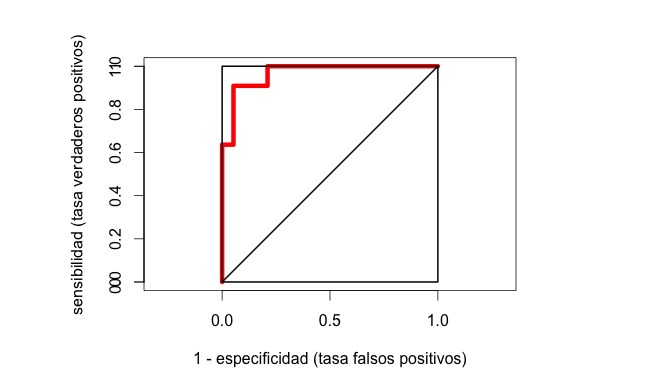
\includegraphics[width=13cm]{../fig/Cap13-CurvaROCvasculopatia.png}
\end{enColor}
\begin{bn}
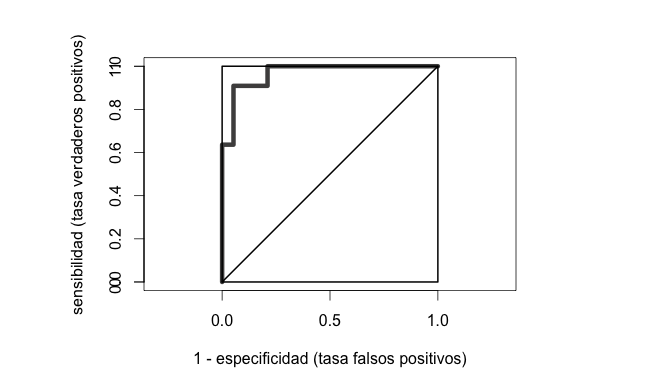
\includegraphics[width=13cm]{../fig/Cap13-CurvaROCvasculopatia-bn.png}
\end{bn}
\caption{La curva ROC del Ejemplo \ref{cap13:ejem:curvaROC2}. }
\label{cap13:fig:curvaROCVasculopatia}
\end{center}
\end{figure}
\qed
\end{ejemplo}

Otra aplicación de las curvas ROC es la de comparar dos métodos de clasificación entre sí.
\begin{ejemplo}
\label{cap13:ejem:CurvasROCcompararClasificadores}
La Figura \ref{cap13:fig:curvaROCdosmodelos} muestra las curvas ROC de los clasificadores knn para $k=5$ (en azul trazo continuo) y para $k=7$ en trazo rojo discontinuo.

\begin{figure}[htb]
\begin{center}
\begin{enColor}
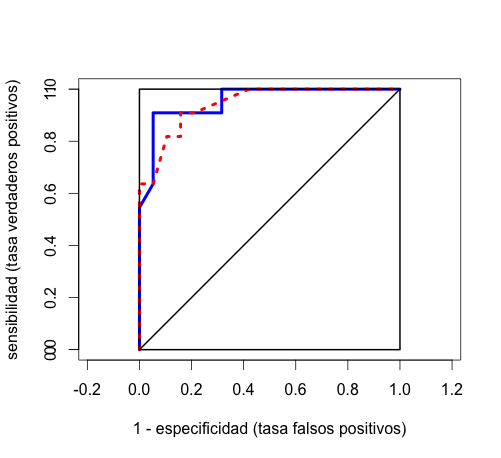
\includegraphics[width=10cm]{../fig/Cap13-CurvaROCvasculopatia02.png}
\end{enColor}
\begin{bn}
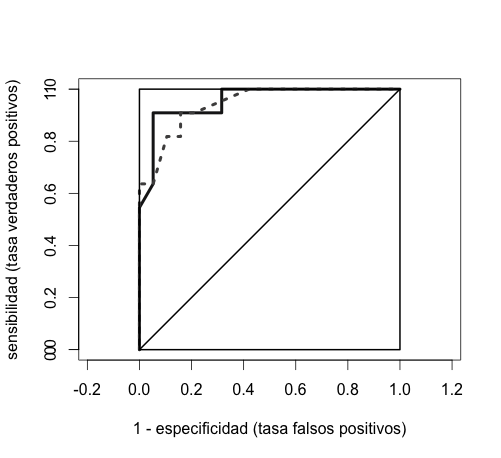
\includegraphics[width=10cm]{../fig/Cap13-CurvaROCvasculopatia02-bn.png}
\end{bn}
\caption{Curvas ROC  para comparar dos clasificadores en el Ejemplo  \ref{cap13:ejem:curvaROC2}. }
\label{cap13:fig:curvaROCdosmodelos}
\end{center}
\end{figure}


Para tratar de aclarar la posible confusión, en cada una de esas curvas se usa un valor de $k$ fijo y es la variación del punto de corte  $c_p$ la que produce los puntos de la curva. Está claro, viendo esas dos curvas,  que los dos clasificadores son distintos. ¿Cuál es mejor? Es posible que la intuición te esté diciendo que el clasificador de la curva azul continua ($k=5$) es mejor que el otro. ¿Pero se te ocurre una manera de comprobarlo?
\qed
\end{ejemplo}


 \subsubsection{Área bajo la curva ROC}

 Como el título de este apartado sugiere,  una de las maneras más sencillas de decidir cuál de las curvas ROC corresponde  a un clasificador mejor es calculando el área bajo la curva. Cuanto mejor sea la curva, en el sentido de que se acerque lo más posible a la esquina superior izquierda, más cerca de $1$ estará el valor del área. Y puesto que comparar el valor de dos números es muy fácil, el área nos brinda un primer criterio muy sencillo para ordenar los clasificadores.  En la literatura científica se suele utilizar el símbolo {\sf AUC}\index{AUC ({\em area under curve}, curvas ROC)} del inglés {\em area under curve} para referirse al área bajo la curva ROC. Hay que tener en cuenta que la curva ROC de cualquier clasificador digno de ese nombre se sitúa siempre por encima  de la diagonal del cuadrado. Y, en consecuencia, $AUC > \frac{1}{2}$.  Algunos autores se apoyan en esto para restar siempre $\frac{1}{2}$ del valor del área. Nosotros preferimos mantener el valor del área tal cual.  Y en el Tutorial13 aprenderemos a obtener su valor con facilidad usando el ordenador.


\begin{ejemplo}
\label{cap13:ejem:AUC}

Cuando se aplican esos métodos a las dos curvas ROC que aparecen en la Figura \ref{cap13:fig:curvaROCdosmodelos} se obtiene un valor $AUC = 0.9545$ para la curva correspondiente a  $k=5$ (en azul trazo continuo) y $AUC = 0.9426$ para la correspondiente a $k=7$ (en trazo rojo discontinuo). Ese resultado puede usarse como criterio para decidir que $k=5$ define un clasificador mejor. De hecho, utilizando esta técnica puede comprobarse que $k=5$ es el mejor valor para el clasificador $knn$ con ese conjunto de datos.
\qed
\end{ejemplo}

\section{Bondad del ajuste en la regresión logística.}
\label{cap13:sec:BondadDelAjuste}
\noindent{\bf Opcional: esta sección puede omitirse en una primera lectura.}\\

A lo largo de este capítulo hemos invitado en varias ocasiones al lector a echar la vista atrás y comparar lo que hacemos aquí con lo que hicimos en el Capítulo \ref{cap:RegresionLinealSimple} para el modelo de regresión lineal simple. Y si el lector ha venido haciendo ese ejercicio con atención, habrá detectado algunas omisiones notables en este capítulo. Hay al menos dos evidentes (y algunas otras de menor trascendencia):

\begin{itemize}
 	\item Empecemos por la diferencia  que vamos a dejar sin resolver: en el   Capítulo \ref{cap:RegresionLinealSimple} dedicamos la Sección \ref{cap10:subsec:ValoresAtipicosPuntosInfluyentesRegresion} (pág. \pageref{cap10:subsec:ValoresAtipicosPuntosInfluyentesRegresion}) al análisis del papel que juegan los valores atípicos y los puntos influyentes en el modelo de regresión lineal simple. Este análisis forma una parte sustancial de lo que se conoce como {\sf diagnóstico del modelo}. Y en el caso de la regresión logística se pueden plantear una discusión muy parecida. Pero en este libro no vamos a entrar en esa discusión, para no hacer el capítulo más extenso de lo que ya es. Remitimos al lector a las referencias que aparecen en el Apéndice \ref{apendice:MasAlla}.

 	\item La otra diferencia tiene que ver con algo que ya comentamos al comienzo de este capítulo: en el Capítulo \ref{cap:RegresionLinealSimple} el modelo era la recta de regresión y la identidad Anova nos servía para medir lo bien que ese modelo estaba haciendo su trabajo. Es decir, para medir la bondad del ajuste entre las predicciones del modelo y los valores observados. En última instancia, era la identidad Anova la que nos servía de base para definir el coeficiente de correlación lineal de Pearson, que es el indicador más básico y más utilizado de la calidad del ajuste de un modelo lineal a los datos muestrales. En el caso de la regresión logística  no disponemos de la identidad Anova y, por tanto, tenemos que buscar otra manera de medir la bondad del ajuste. Eso es lo que vamos a hacer en esta sección.
\end{itemize}

Y aunque hemos planteado el problema comparando el Capítulo \ref{cap:RegresionLinealSimple} con este, el lector habrá notado que el lenguaje del párrafo anterior se ha deslizado la noción de {\em bondad del ajuste}, que a su vez nos debe hacer pensar en el Capítulo \ref{cap:TablasContingenciaTestChi2}. 	La elección de la terminología no ha sido, desde luego, accidental, porque el método que vamos a usar le recordará al lector, inevitablemente, al contraste $\chi^2$ de homogeneidad  que vimos en la Sección \ref{cap12:sec:ChiCuadradoHomgeneidad} y que también llamamos contraste para la bondad del ajuste. Tampoco es accidental que hayamos pospuesto esta sección hasta haber discutido los problemas de clasificación en la Sección \ref{cap13:sec:ValorPredictivo}. La clasificación tiene mucha relación con la bondad del ajuste, como trataremos de poner de manifiesto.

Por último, antes de empezar con los detalles, {\bf una advertencia:} para hacer este análisis de bondad del ajuste vamos a cerrar un poco el foco. Recuerda que en el modelo concreto de regresión logística que estamos discutiendo, la variable respuesta es $Y$ es dicotómica (o de Bernouilli) mientras que la variable explicativa $X$ es cuantitativa, ya sea discreta o continua. Y aunque la mayoría de los ejemplos de este Capítulo involucraban variables $X$ que considerábamos continuas lo cierto es que buena parte de lo que  hemos visto sobre el modelo de regresión logística se aplica sin demasiadas diferencias cuando $X$ es discreta. Como, por otra parte,
ya habíamos anunciado al comienzo de este capítulo, en la Sección \ref{cap13:sec:IntroduccionProblemaRegresionLogistica} (\pageref{cap13:sec:IntroduccionProblemaRegresionLogistica}).  Sin embargo, en esta sección {\bf vamos a  limitarnos a considerar el caso en el que la variable $X$ es continua y, además, asumiremos que  la muestra contiene suficientes observaciones} como para llevar adelante el método que vamos a describir.
Las razones para imponer estas condiciones son puramente estratégicas: el caso que vamos a estudiar contiene los ingredientes esenciales del problema, pero elimina algunas dificultades técnicas que pueden presentarse cuando $X$ es  discreta

\subsection{Clases decílicas y estadístico de Hosmer-Lemeshow.}

¿Qué significa la bondad del ajuste en la regresión logística? Para contestar a la pregunta vamos a generalizarla un poco y la formularemos de esta manera: ¿qué significa la bondad del ajuste en un modelo estadístico en general?

\subsubsection*{Indicadores globales de la bondad del ajuste de un modelo.}

Para empezar a entender la respuesta, volvamos sobre nuestro encuentro con la idea de bondad del ajuste en el Capítulo \ref{cap:TablasContingenciaTestChi2}. En aquel capítulo un buen ajuste significaba que las frecuencias observadas se parecían a las probabilidades que predecía la hipótesis nula. Una forma útil de pensar en esto es darse cuenta de que allí  {\em la hipótesis nula era el modelo} que hacía predicciones sobre las probabilidades.  Así que es fácil cambiar ligeramente la frase para obtener una noción más general: {\em un buen ajuste del modelo  significa que la distribución observada de la variable respuesta se parece mucho a las probabilidades que predice el modelo.}

Puestas así las cosas, hay dos formas evidentes de abordar el problema del ajuste del modelo, que se corresponden con los dos puntos con los que hemos abierto esta sección. Una forma consiste en estudiar las probabilidades individualmente, haciendo lo que hemos llamado un diagnóstico del modelo y estudiando los valores atípicos, puntos influyentes, etc. Pero ya hemos dicho que no nos vamos a internar por ese camino. Otra forma consiste en buscar un resumen global del ajuste del modelo, un  número que nos permita hacernos una idea inicial de la situación. En el modelo de regresión lineal el coeficiente de correlación $R$ jugaba ese papel. Recuerda que allí dijimos que un valor alto de $R$ no significaba automáticamente que el modelo fuera bueno. En cambio, un valor bajo era una garantía de que el modelo no estaba haciendo bien su trabajo. Lo que vamos a hacer es buscar una herramienta similar para el modelo de regresión logística que nos sirva como una prueba preliminar global del modelo. Si el modelo pasa esa prueba, entonces podemos seguir adelante con un diagnóstico más detallado.

\subsubsection*{Valores observados y esperados.}

¿Cómo podemos construir ese indicador global? En la regresión lineal pensábamos en la diferencia entre los valores observados de la variable respuesta $y_i$ y los valores esperados, que son los valores predichos por el modelo, los $\hat y_i$. Y entonces estudiamos el error cuadrático, que era una representación global de esas diferencias:
\begin{equation}\tag{\ref{cap10:ecu:ErrorCuadratico} repetida}
\mbox{EC} = \sum_{i=1}^n(y_i-\hat y_i)^2.
\end{equation}
Naturalmente, después tuvimos que hacer mucho más trabajo. Pero queremos llamar la atención del lector sobre el hecho fundamental de que la idea básica de la bondad del ajuste ya estaba presente: {\em se trata de comparar valores observados frente a valores predichos por el modelo.}

Un problema, al tratar de trasladar estas ideas al caso de la regresión logística, es que en este caso el modelo no predice valores de $Y$ sino probabilidades. Así que vamos a tener que traducir de alguna manera las probabilidades en valores esperados. En realidad, el trabajo que tenemos que hacer se parece mucho a lo que ya hicimos en el Ejemplo Ejemplo
\ref{cap13:ejem:EstimacionModeloLogisticoMedianteClases}
(pág.  \pageref{cap13:ejem:EstimacionModeloLogisticoMedianteClases}), cuando estábamos empezando a construir el modelo logístico.  Así que antes de seguir adelante, te recomendamos que repases ese ejemplo, en el que se describía un procedimiento para estimar las probabilidades:

\begin{enumerate}
	\item El punto de partida es la muestra
	\[(x_1, y_1), (x_2, y_2), \ldots, (x_n, y_n)\]
	\item En primer lugar agrupábamos los valores de $X$ en intervalos (clases). Vamos a llamar $C_1, \ldots, C_k$ a esas clases.
	\item Para cada una de esas clases, sea $n_i$ el número de valores de $X$ que pertenecen a la clase $C_i$.
	\item Hicimos una estimación de la probabilidad común para todos los valores de la clase $C_i$ que se podía expresar así:
	\[\hat p_i = \dfrac{\displaystyle\sum_{x_j\in C_i} y_j}{n_i}.\]
	Es decir, sumábamos los valores (unos y ceros) de la variable $Y$ correspondientes a los puntos $x_i$ en  ese intervalo y dividíamos por el número de puntos. Esta ecuación es otra forma de expresar la Ecuación \ref{cap13:ecu:EstimacionProbabilidadFactorIgual1EnUnaClase} (pág. \pageref{cap13:ecu:EstimacionProbabilidadFactorIgual1EnUnaClase}).
\end{enumerate}

Hay dos aspectos de ese procedimiento sobre los que queremos detenernos:

\begin{itemize}
\item Empezando por el último paso, ahora lo que necesitamos es calcular el número de valores observados en cada clase. Así que haremos la misma suma de valores de $Y$ para los puntos $x_i$  de cada clase, pero no vamos a dividir por $n_j$. Llamaremos $O_i$ al valor resultante, donde la $O_i$ desde luego significa que son los valores observados correspondientes al intervalo número $i$.

\item Pero el paso clave es la construcción de las clases. Ya nos hemos encontrado antes con este problema: ¿cómo se deben agrupar en clases los valores de una variable continua? Recuerda, por ejemplo, la construcción del histograma en el Sección \ref{cap01:sec:Histogramas} (pág. \pageref{cap01:sec:Histogramas}). En el Ejemplo \ref{cap13:ejem:EstimacionModeloLogisticoMedianteClases} lo que hicimos fue dividir el recorrido de los valores $x_i$ en intervalos  de la misma longitud. Por lo tanto la división en clases se hace sin prestar atención a la distribución de la variable $Y$ en la muestra. Y eso no parece una gran idea si lo que queremos es medir la calidad de nuestras predicciones sobre esa variable.

\end{itemize}

La idea que vamos a usar para la construcción del estadístico del contraste de Hosmer - Lemeshow parte de esta última observación. Construir las clases significa clasificar los valores $x_i$. Pero en lugar de hacerlo por el valor de la variable $x_i$, lo que vamos a hacer es clasificarlos {\em por el valor de las probabilidades $\hat{\pi}(x_i)$ que estima el modelo logístico}. De esa forma, la clasificación incorpora la información sobre la variable $Y$.


\subsubsection*{La construcción del estadístico de Hosmer - Lemeshow, paso a paso.}
\label{cap13:subsubsec:ConstruccionEstadisticoHosmerLemeshowPasoPaso}

Vamos a ver detenidamente como construimos los valores observados y esperados que intervienen en el estadístico de Hosmer-Lemeshow que usaremos como indicador global de la bondad del ajuste para el modelo logístico:

\begin{enumerate}
\item Dadas las probabilidades $\hat{\pi}(x_i)$ que el modelo estima para los puntos de la muestra, elegimos un número $g$ de clases (se suele utilizar $g = 10$) y calculamos los correspondientes percentiles de las probabilidades estimadas. Insistimos: de las probabilidades, no de los $x_i$. Supongamos, para fijar ideas, que usamos el valor típico $g=10$. Entonces obtendremos $10$ valores:
    \[ p_1 < p_2 < p_3 < \cdots < p_{10}\]
    tales que: un 10\% de los valores $x_i$ tienen {\em probabilidades estimadas} más bajas que $p_1$; otro 10\% de los $x_i$ tienen {\em probabilidades estimadas} comprendidas entre $p_1$ y $p_2$, etc. A riesgo de parecer reiterativos, hemos destacado que lo que se usa para clasificar un valor $x_i$ es la probabilidad estimada $\hat{\pi}(x_i)$ que el modelo asigna a ese valor, y no el propio valor $x_i$. El resultado de este paso es una colección de $g$ clases, a las que llamaremos $C_1, C_2, \ldots, C_g$. Usando terminología procedente de la Epidemiología, estas clases se suelen llamar {\sf clases de riesgo}\index{riesgo, clases de}\index{clases de riesgo}. Y en el caso frecuente en el que $g = 10$, se denominan {\sf deciles de riesgo}\index{riesgo, deciles de}\index{deciles de riesgo} (del inglés, {\em deciles of risk}\index{risk, deciles of}\index{deciles of risk}). Los deciles de riesgo son, en realidad, los valores que separan una clase de la siguiente, pero a menudo identificaremos cada clase con el decil que marca su extremo superior. El origen de la terminología de {\em riesgo} está claro: si $Y=1$ significa {\em enfermo}, entonces la clase $C_1$ contiene a aquellos individuos a los que el modelo les asigna una probabilidad o riesgo más bajo de enfermar, mientras que $C_g$ la forman los individuos con un riesgo de enfermedad más alto. Los números $m_1, m_2, \ldots, m_g$ indican el número de individuos que forman cada una de las clases.

    \begin{ejemplo}
    \label{cap13:ejem:hosmerlemeshow01}
    Cuando se aplican estas ideas a los datos del Ejemplo \ref{cap13:ejem:EstimacionModeloLogisticoMedianteClases} (pág. \pageref{cap13:ejem:EstimacionModeloLogisticoMedianteClases}) se obtienen para los deciles de riesgo los valores que aparecen en la Tabla \ref{cap13:tabla:hosmerlemeshow01}, como veremos en el Tutorial13. La tabla también contiene los valores $m_1, \ldots, m_{10}$.

        \begin{table}[htbp]
            \begin{center}
            \begin{tabular}{rlrr}
              \hline
             $i$ & Porcentaje & Decil & $m_i$ \\
              \hline
               %0\% & $2.53\cdot 10^{-5}$ & 100\\
               1 & 10\% & $0.0002547$& 100 \\
               2 &  20\% & 0.00185& 100 \\
               3 &  30\% & 0.0153& 100 \\
               4 &  40\% & 0.129& 100 \\
               5 & 50\% & 0.581& 99 \\
               6 & 60\% & 0.924& 101 \\
               7 & 70\% & 0.986& 100 \\
               8 & 80\% & 0.998& 100 \\
               9 &  90\% & 0.9998& 100 \\
               10&  100\% & 1.00& 100 \\
               \hline
            \end{tabular}
            \end{center}
        	\caption{Deciles de riesgo del Ejemplo \ref{cap13:ejem:hosmerlemeshow01}.}
            \label{cap13:tabla:hosmerlemeshow01}
        \end{table}
    \end{ejemplo}

\item Ahora volvemos a conectar con la idea del Ejemplo \ref{cap13:ejem:EstimacionModeloLogisticoMedianteClases}. Para cada clase $C_i$ definimos el número de valores $Y=1$ observados $Obs1_i$ correspondiente a esa clase mediante:
    \begin{equation}
    \label{cap13:ecu:Obs1HosmerLemeshow}
    Obs1_i = \displaystyle\sum_{x_j\in C_i} y_j.
    \end{equation}
    Naturalmente, puesto que los valores $x_i$ se han clasificado por riesgo, esperamos que los $Obs1_i$ correspondientes a las primeras clases sean bajos, y los de las últimas clases sean altos.

    \begin{ejemplo}
    \label{cap13:ejem:hosmerlemeshow02}
    {\bf (Continuación del Ejemplo \ref{cap13:ejem:hosmerlemeshow01}, pág. \pageref{cap13:ejem:hosmerlemeshow01})}
    En el Tutorial13 veremos que los valores observados $Obs1_i$ para cada una de las clases decílicas son los que aparecen en la tercera columna de la Tabla \ref{cap13:tabla:hosmerlemeshow02}.
    \begin{table}[ht]
    \begin{center}
    \begin{tabular}{llrrrrr}
      \hline
     & Clase de riesgo & $Obs1_i$ & $Esp1_i$ & $Obs0_i$ & $Esp0_i$ & $m_i$ \\
      \hline
      1 & [0,0.0002547] &   0 & 0.01 & 100 & 99.99 & 100 \\
      2 & (0.0002547,0.001877] &   0 & 0.08 & 100 & 99.92 & 100 \\
      3 & (0.001877,0.0158] &   0 & 0.67 & 100 & 99.33 & 100 \\
      4 & (0.0158,0.1312] &   6 & 5.31 &  94 & 94.69 & 100 \\
      5 & (0.1312,0.581] &  35 & 33.22 &  65 & 66.78 & 100 \\
      6 & (0.581,0.9236] &  74 & 77.28 &  25 & 21.72 &  99 \\
      7 & (0.9236,0.9862] &  98 & 97.10 &   3 & 3.90 & 101 \\
      8 & (0.9862,0.9982] & 100 & 99.42 &   0 & 0.58 & 100 \\
      9 & (0.9982,0.9998] & 100 & 99.92 &   0 & 0.08 & 100 \\
      10 & (0.9998,1] & 100 & 99.99 &   0 & 0.01 & 100 \\
       \hline
    \end{tabular}
    \end{center}
    \caption{Valores $Obs1_i$ en el Ejemplo \ref{cap13:ejem:hosmerlemeshow02}.}
    \label{cap13:tabla:hosmerlemeshow02}
    \end{table}

\end{ejemplo}

\item Los $Obs1_i$ son valores observados. ¿Cuáles son los valores esperados correspondientes? Es decir, ¿cuál es el número esperado (predicho) $Esp1_i$ de individuos con $Y=1$ dentro de la clase $C_i$? Y esta es la otra idea importante del método: podemos estimar ese número sin más que sumar las probabilidades estimadas $\hat{\pi}(x_i)$ para los individuos de esa clase. Para entenderlo, piensa en un caso simplificado. Imagínate que la clase de riesgo $C_4$ contiene $20$ individuos y que el modelo dice que todos ellos tienen la misma probabilidad del $40\%$ de que sea $Y=1$. ¿Cuántos valores $Y=1$ esperarías encontrar en ese grupo? Puesto que las observaciones son independientes, podemos usar lo que sabemos de la binomial para concluir que esperaríamos:
    \[20 \cdot 0.4 = 8.\]
    Ese sería el valor esperado $E_4$ en este caso, en el que para simplificar hemos supuesto que la probabilidad estimada $\hat{\pi}(x_i)$ es la misma ($40\%$) para todos los casos de la clase de riesgo $C_4$. En una situación más realista, un individuo de $C_4$ puede tener una probabilidad estimada del $32\%$, otro del $37\%$, etcétera. En este caso ya no podemos usar una cuenta sencilla basada en la binomial como antes, pero el remedio tampoco es demasiado complicado: la forma de estimar el valor esperado total para esa clase es {\em sumando todas las probabilidades estimadas para los individuos de esa clase de riesgo}. Eso nos lleva a esta expresión para los valores esperados:
    \begin{equation}
    \label{cap13:ecu:Esp1HosmerLemeshow}
    Esp1_i = \displaystyle\sum_{x_j\in C_i} \hat{\pi}(x_j).
    \end{equation}
    \begin{ejemplo}
    \label{cap13:ejem:hosmerlemeshow03}
    {\bf (Continuación del Ejemplo \ref{cap13:ejem:hosmerlemeshow02}, pág. \pageref{cap13:ejem:hosmerlemeshow02})}
    Los valores esperados $Esp1_i$ para el ejemplo que venimos analizando aparecen en la cuarta columna de la Tabla \ref{cap13:tabla:hosmerlemeshow02}, como veremos en el Tutorial13.
    \end{ejemplo}


\item Además de los valores observados y esperados para $Y=1$, debemos también obtener los valores observados y esperados para $Y=0$. Afortunadamente, puesto que sabemos cuántos individuos hay en cada clase, esos valores se obtienen simplemente restando:
    \begin{equation}
    \label{cap13:ecu:ObsEsp0HosmerLemeshow}
    \begin{cases}
    Obs0_i = m_i - Obs1_i\\[3mm]
    Esp0_i = m_i - Esp1_i
    \end{cases}
    \end{equation}


    \begin{ejemplo}
    \label{cap13:ejem:hosmerlemeshow04}
    {\bf (Continuación del Ejemplo \ref{cap13:ejem:hosmerlemeshow03}, pág. \pageref{cap13:ejem:hosmerlemeshow03})}
    Estos dos conjuntos de valores completan la Tabla \ref{cap13:tabla:hosmerlemeshow02} de nuestro ejemplo, y aparecen en las columnas cuarta y quinta de la tabla.
    \end{ejemplo}

\end{enumerate}
Una vez disponemos de los valores observados y esperados estamos listos para calcular el valor del estadístico de Hosmer-Lemeshow. \\[3mm]
\fcolorbox{black}{Gris025}{
\begin{minipage}{12cm}
\begin{center}
    {\bf Estadístico de Hosmer - Lemeshow.  }\\
    {\bf Contraste de bondad del ajuste en regresión logística.}\\
\end{center}
Si los valores de la muestra se han agrupado en $g$ clases de riesgo, y los valores observados y esperados se calculan como se ha explicado en las Ecuaciones \ref{cap13:ecu:Obs1HosmerLemeshow},  \ref{cap13:ecu:Esp1HosmerLemeshow} y \ref{cap13:ecu:ObsEsp0HosmerLemeshow}, entonces el estadístico de Hosmer - Lemeshow se define mediante:
\begin{equation}
{\cal HL} =
\sum_{i = 1}^g \dfrac{(Obs1_i - Esp1_i)^2}{Esp_1} +
\sum_{i = 1}^g \dfrac{(Obs0_i - Esp0_i)^2}{Esp_0}
\end{equation}
Además, si la hipótesis nula
\[H_0 =
\{\mbox{El modelo
logístico predice bien las probabilidades
observadas.}\}\]
es cierta, entonces el estadístico ${\cal HL}$ se distribuye como una $\chi^2_{g - 2}$.
\end{minipage}
}\\[3mm]
En particular si, como es habitual, se utilizan clases decílicas de riesgo,  entonces ${\cal HL}$ se distribuye como una $\chi^2_8$.

\begin{ejemplo}
\label{cap13:ejem:hosmerlemeshow05}
{\bf (Continuación del Ejemplo \ref{cap13:ejem:hosmerlemeshow04}, pág. \pageref{cap13:ejem:hosmerlemeshow04})}
Usando los valores  de la Tabla \ref{cap13:tabla:hosmerlemeshow02}  se obtiene este valor del estadístico:
\[
{\cal HL} = 2.516
\]
Y entonces, calculando la cola derecha de la distribución $\chi^2_8$ para ese valor de ${\cal HL}$ se obtiene un p - valor aproximadamente igual a $0.96$. El p-valor tan cercano a uno nos dice que desde luego no debemos rechazar la hipótesis nula $H_0$. Y eso, en el contexto del contraste sobre la bondad del ajuste, significa que no tenemos razones para sospechar de la bondad del ajuste de las predicciones del modelo a los datos observados. El modelo parece estar haciendo bien su trabajo. Al menos globalmente, como enseguida vamos a discutir.
\qed
\end{ejemplo}

{\bf Atención:} Como hemos visto en este ejemplo, en un contraste de Hosmer-Lemeshow los valores del p-valor cercanos a uno (y no a cero, como en otros casos) son los que nos garantizan un buen ajuste del modelo a los datos.

Nuestra discusión de los métodos para medir la bondad del ajuste de un modelo de regresión logística es meramente introductoria, por razones de espacio y porque el lugar natural para una discusión más completa un curso centrado en el modelo de regresión  logística. Un curso en el que, por ejemplo, se haya discutido en profundidad cómo se construye ese modelo en presencia de varias variables explicativas, que pueden ser factores o variables cuantitativas (tanto discretas como
continuas). Nosostros vamos a cerrar aquí nuestra incursión en este modelo, con tan sólo un par de obsevaciones finales:

\begin{itemize}
	\item El contraste de Hosmer - Lemeshow es una medida {\sf global} o {\sf medida resumen} de la bondad del ajuste del modelo. Es importante entender que ese contraste no proporciona una medida de la calidad de las {\em predicciones individuales} del modelo para cada valor observado de la variable explicativa. Es decir, que aunque el contraste de Hosmer-Lemeshow no sea significativo, todavía puede ocurrir que alguna de las predicciones del modelo (valores esperados) se aleje de los valores observados. Para entrar a valorar ese ajuste a nivel individual es necesario un análisis similar al análisis de los residuos que hacíamos en el Capítulo \ref{cap:RegresionLinealSimple} y la discusión de conceptos como el de valores atípicos, puntos influyentes, etc.
	
	\item El estadístico de Hosmer-Lemeshow, como muchos otros que  hemos visto en capítulos anteriores, se basa  en el comportamiento {\em asintótico} de la distribución muestral; en otras palabras, en lo que sucede cuando las muestras aleatorias son suficientemente grandes. Si las muestras son pequeñas, las cosas son más complicadas. La situación es parecida a la que hemos encontrado en el Capítulo \ref{cap:TablasContingenciaTestChi2} (ver página \pageref{cap12:ecu:ContrasteChi2Homogeneidad}), en el que para aplicar el contraste $\chi^2$ de homogeneidad  poníamos como condición que ninguno de los valores esperados en la tabla de contingencia fuese menor que $5$.  En el modelo de regresión logística, cuando las muestras son pequeñas (como sucede en el Ejemplo \ref{cap13:ejem:RegresionLogistica00}, pág. \pageref{cap13:ejem:RegresionLogistica00}), se aplican condiciones similares sobre la validez del contraste. Alternativamente, se pueden utilizar otros métodos, similares a los métodos exactos que hemos visto en otros capítulos.
\end{itemize}
En cualquier caso, el lector interesado encontrará más información en las referencias que se incluyen en el Apéndice \ref{apendice:MasAlla}.

